% !TEX program = xelatex
\documentclass[UTF8,fontset=fandol,a4paper,11pt]{ctexart}
\usepackage[margin=21mm,top=23mm,bottom=22mm,headheight=16pt]{geometry}
\usepackage{amsmath,amssymb,mathtools,bm}
\usepackage{tikz}
\usetikzlibrary{arrows.meta,calc,angles,quotes,patterns}
\usepackage{xcolor,booktabs,array,longtable,enumitem,fancyhdr,needspace}
\usepackage[unicode,hidelinks]{hyperref}
\definecolor{ink}{HTML}{24343C}
\definecolor{accent}{HTML}{166A70}
\definecolor{muted}{HTML}{65747A}
\definecolor{rulegray}{HTML}{D4DDE0}
\definecolor{warm}{HTML}{966037}
\color{ink}
\setlength{\parindent}{2em}
\setlength{\parskip}{4pt}
\linespread{1.12}
\AtBeginDocument{\setlength{\abovedisplayskip}{6pt plus 2pt minus 1pt}
\setlength{\belowdisplayskip}{6pt plus 2pt minus 1pt}
\setlength{\abovedisplayshortskip}{0pt plus 1pt}
\setlength{\belowdisplayshortskip}{4pt plus 1pt}}
\setlist[enumerate]{label=(\arabic*),leftmargin=2.3em,itemsep=3pt,topsep=4pt}
\setlist[itemize]{leftmargin=2em,itemsep=2pt,topsep=4pt}
\allowdisplaybreaks[1]
\setlength{\emergencystretch}{2em}
\setcounter{secnumdepth}{0}
\providecommand{\tightlist}{\setlength{\itemsep}{0pt}\setlength{\parskip}{0pt}}
\ctexset{section={format=\Large\bfseries\color{accent},beforeskip=10pt,afterskip=9pt},
subsection={format=\normalsize\bfseries\color{accent},beforeskip=10pt,afterskip=4pt},
subsubsection={format=\normalsize\bfseries,beforeskip=8pt,afterskip=3pt}}
\pagestyle{fancy}
\fancyhf{}
\fancyhead[L]{\small\color{muted}物理学难题集萃}
% 页眉仅保留书名；版本名称只在封面显示。
\fancyfoot[L]{\small\color{muted}\chapterlabel}
\fancyfoot[R]{\small\thepage}
\renewcommand{\headrulewidth}{0.4pt}
\renewcommand{\footrulewidth}{0pt}
\newcommand{\dd}{\mathop{}\!\mathrm{d}}
\newcommand{\vect}[1]{\bm{#1}}
\newcommand{\tagline}[1]{\noindent{\small\color{muted}#1}\par}
\newcommand{\result}[1]{\begin{equation*}\boxed{#1}\end{equation*}}
\newcommand{\figcaption}[1]{\par\vspace{2pt}{\small\color{muted}#1}\par}
\newcommand{\teach}[2]{\Needspace{4\baselineskip}\subsection*{讲解要点与追问}#1\par\smallskip\noindent\textbf{追问：}#2\par}
\newcommand{\workarea}{\par\vspace{7mm}\noindent{\small\color{muted}作答区}\par\vspace{4mm}
\noindent\textcolor{rulegray}{\rule{\linewidth}{0.3pt}}\par\vspace{16mm}
\noindent\textcolor{rulegray}{\rule{\linewidth}{0.3pt}}\par\vspace{16mm}
\noindent\textcolor{rulegray}{\rule{\linewidth}{0.3pt}}\par\vspace{16mm}
\noindent\textcolor{rulegray}{\rule{\linewidth}{0.3pt}}}
\tikzset{axis/.style={-{Stealth[length=2mm]},thin,color=muted},
motion/.style={-{Stealth[length=2.3mm]},thick,color=accent},
force/.style={-{Stealth[length=2.3mm]},thick,color=warm},
traj/.style={thick,color=accent},guide/.style={dashed,thin,color=muted},
object/.style={thick,color=ink},every node/.style={font=\small}}\widowpenalty=10000\clubpenalty=10000\displaywidowpenalty=10000\newcommand{\chapterlabel}{电磁学试题（四）}







\hypersetup{pdftitle={电磁学试题（四）·教师版},pdfauthor={}}

\begin{document}\pdfbookmark[0]{电磁学试题（四）}{cover}

\thispagestyle{empty}\vspace*{22mm}

\noindent{\Huge\bfseries 物理学难题集萃}\par\vspace{12mm}

\noindent{\LARGE 电磁学试题（四）}\par\vspace{12mm}

\noindent{\Large\color{accent}教师版}\par\vspace{9mm}

\noindent\textcolor{accent}{\rule{\linewidth}{1pt}}\par\vspace{9mm}

\noindent 第1--5题\par\vfill\clearpage

\pdfbookmark[1]{题目目录}{contents}\section*{题目目录}

\begin{longtable}{@{}r p{113mm} r@{}}\toprule 题号 & 题目 & 页码\\\midrule

\hyperref[q:1]{1} & \hyperref[q:1]{非均匀导体中的体电荷与界面电荷} & \pageref{q:1} \\

\hyperref[q:2]{2} & \hyperref[q:2]{多端等效与无限内接三角形网络} & \pageref{q:2} \\

\hyperref[q:3]{3} & \hyperref[q:3]{互补RL、RC支路的相量与初始储能} & \pageref{q:3} \\

\hyperref[q:4]{4} & \hyperref[q:4]{双行CLC网络的复阻抗和功率因数} & \pageref{q:4} \\

\hyperref[q:5]{5} & \hyperref[q:5]{导体屏蔽暂态与单频等效电容} & \pageref{q:5} \\

\bottomrule\end{longtable}

\clearpage

\pdfbookmark[2]{第 1 题 非均匀导体中的体电荷与界面电荷}{q1}

\section*{第 1 题\quad 非均匀导体中的体电荷与界面电荷}\label{q:1}


长为$L$、截面积为$S$的均匀粗细导体，沿轴线$x$的电阻率为
\[
\rho(x)=\rho_0\left|\sin\frac{2\pi x}{L}\right|,\qquad 0\le x\le L.
\]
导体两端保持电势差$V(0)-V(L)=U>0$，已达稳恒状态。采用一维导电模型，电场沿轴线，电荷关系用$\varepsilon_0$描述。
\begin{enumerate}
\item 求导体电阻和电流密度。
\item 求内部体电荷密度$\rho_e(x)$，指出带正电的区段。
\item $x=L/2$处体电荷密度发生跳变，该截面上是否存在面电荷？给出判断依据。
\end{enumerate}


\begin{center}\begin{minipage}{.98\linewidth}\centering
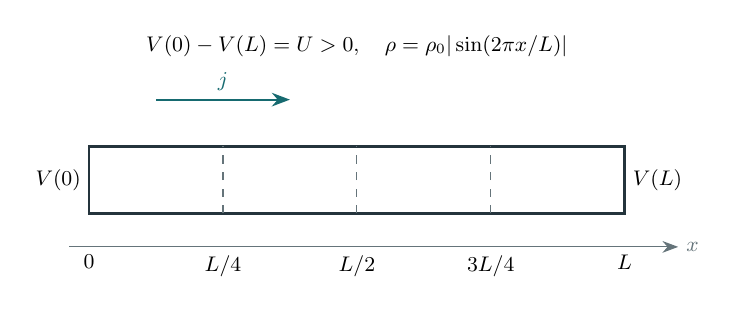
\begin{tikzpicture}[scale=.85,transform shape]

\draw[object] (0,-.5) rectangle (8,.5);
\foreach \x in {2,4,6}{\draw[guide] (\x,-.5)--(\x,.5);}
\draw[motion] (1,1.2)--(3,1.2) node[midway,above] {$j$};
\draw[axis] (-.3,-1)--(8.8,-1) node[right] {$x$};
\foreach \x/\l in {0/0,2/{L/4},4/{L/2},6/{3L/4},8/L}{\node[below] at (\x,-1) {$\l$};}
\node[left] at (0,0) {$V(0)$};\node[right] at (8,0) {$V(L)$};
\node at (4,2) {$V(0)-V(L)=U>0,\quad \rho=\rho_0|\sin(2\pi x/L)|$};

\end{tikzpicture}
\figcaption{图电试4.1\quad 同截面微段串联，稳恒电流沿轴向。}
\end{minipage}\end{center}

\Needspace{8\baselineskip}

\pdfbookmark[3]{题型定位}{q1-h0}

\subsection*{题型定位}

非均匀导体的稳恒导电与空间电荷。电流连续性先给各截面相同的$j$，局部欧姆定律确定随电阻率变化的电场，再由高斯定律分别求体电荷与截面电荷。体电荷对应电场的空间导数，面电荷对应电场法向分量的左右差值，二者在同一高斯薄层中联系起来。

\Needspace{8\baselineskip}

\pdfbookmark[3]{知识点}{q1-h1}

\subsection*{知识点}

无侧向漏流且截面积恒定时，稳恒电流密度处处相同。串联微元$dR=\rho\mathrm dx/S$用绝对值函数分段积分。电场沿轴向，局部关系$E_x=\rho j$与总电压积分相容。一维高斯定律给$\rho_e=\varepsilon_0E_x'$，跨截面薄柱则给$\sigma=\varepsilon_0(E_+-E_-)$。电势是负电场积分，有界体电荷在无限薄层内的总量随厚度趋零。

\Needspace{8\baselineskip}

\pdfbookmark[3]{物理图像}{q1-h2}

\subsection*{物理图像}

题图的等截面圆柱中，每个截面通过同一电流。解图电试4.1A的电场有两个正半波，在中点连续降到零；图D把两个开区间的电荷曲线分开，左右极限分别为$-K,+K$。图B的高斯薄柱突出两端轴向通量与侧面零通量，图C则显示电势降单调累积，在电场为零的中点斜率也为零。

\Needspace{8\baselineskip}

\pdfbookmark[3]{解题入口}{q1-h3}

\subsection*{解题入口}

从任意两个截面之间的电荷不再积累出发，说明$I$与$j$恒定，再算串联电阻积分。场强由电阻率乘$j$给出，在$0<x<L/2$和$L/2<x<L$分别求导。确定正电区后，以中点为中心取轴向高斯薄柱，使用场值左右极限得到截面电荷。

\Needspace{8\baselineskip}

\pdfbookmark[3]{标准解法}{q1-h4}

\subsection*{标准解法}


图电试4.1的圆柱侧面无漏流，任意两截面间的电荷在稳恒状态下保持不变，因此两截面的电流相同。截面积$S$也相同，故$j=I/S$处处相同。取$x$到$x+\mathrm dx$的薄段，其电阻$\mathrm dR=\rho(x)\mathrm dx/S$，各段首尾串联。前半段正弦非负、后半段正弦非正，两段绝对值积分相等；具体地，$\int_0^{L/2}\sin(2\pi x/L)\mathrm dx=L/\pi$。于是
\[
R=\frac{\rho_0}{S}\int_0^L\left|\sin\frac{2\pi x}{L}\right|dx
=\boxed{\frac{2\rho_0L}{\pi S}},\qquad
\boxed{j=\frac{U}{RS}=\frac{\pi U}{2\rho_0L}}.
\]
电流由$x=0$流向$x=L$。材料电阻率的变化由不同的局部场补偿，欧姆定律给
\[
\boxed{E_x(x)=\rho(x)j=\frac{\pi U}{2L}
\left|\sin\frac{2\pi x}{L}\right|}.
\]
\begin{center}\begin{minipage}{.98\linewidth}\centering
\begin{tikzpicture}[scale=.8,transform shape]
\draw[axis] (0,0)--(10.7,0) node[right] {$x/L$};
\draw[axis] (0,0)--(0,3.2) node[above] {$E_xL/U$};\foreach \y/\lab in {0/0,0.9/0.5,1.8/1,2.7/1.5}{\draw[thin] (0,\y)--(-.08,\y) node[left] {$\lab$};}
\node[above] at (5,3.5) {电场沿$+x$，中点连续降到零};
\draw[traj] plot coordinates {(0.000000000,0.000000000) (0.062500000,0.111004514) (0.125000000,0.221837867) (0.187500000,0.332329162) (0.250000000,0.442308030) (0.312500000,0.551604890) (0.375000000,0.660051216) (0.437500000,0.767479791) (0.500000000,0.873724967) (0.562500000,0.978622923) (0.625000000,1.082011914) (0.687500000,1.183732520) (0.750000000,1.283627897) (0.812500000,1.381544012) (0.875000000,1.477329887) (0.937500000,1.570837826) (1.000000000,1.661923647) (1.062500000,1.750446903) (1.125000000,1.836271096) (1.187500000,1.919263892) (1.250000000,1.999297322) (1.312500000,2.076247981) (1.375000000,2.149997216) (1.437500000,2.220431311) (1.500000000,2.287441662) (1.562500000,2.350924943) (1.625000000,2.410783269) (1.687500000,2.466924341) (1.750000000,2.519261596) (1.812500000,2.567714331) (1.875000000,2.612207837) (1.937500000,2.652673508) (2.000000000,2.689048948) (2.062500000,2.721278070) (2.125000000,2.749311179) (2.187500000,2.773105048) (2.250000000,2.792622991) (2.312500000,2.807834912) (2.375000000,2.818717355) (2.437500000,2.825253540) (2.500000000,2.827433388) (2.562500000,2.825253540) (2.625000000,2.818717355) (2.687500000,2.807834912) (2.750000000,2.792622991) (2.812500000,2.773105048) (2.875000000,2.749311179) (2.937500000,2.721278070) (3.000000000,2.689048948) (3.062500000,2.652673508) (3.125000000,2.612207837) (3.187500000,2.567714331) (3.250000000,2.519261596) (3.312500000,2.466924341) (3.375000000,2.410783269) (3.437500000,2.350924943) (3.500000000,2.287441662) (3.562500000,2.220431311) (3.625000000,2.149997216) (3.687500000,2.076247981) (3.750000000,1.999297322) (3.812500000,1.919263892) (3.875000000,1.836271096) (3.937500000,1.750446903) (4.000000000,1.661923647) (4.062500000,1.570837826) (4.125000000,1.477329887) (4.187500000,1.381544012) (4.250000000,1.283627897) (4.312500000,1.183732520) (4.375000000,1.082011914) (4.437500000,0.978622923) (4.500000000,0.873724967) (4.562500000,0.767479791) (4.625000000,0.660051216) (4.687500000,0.551604890) (4.750000000,0.442308030) (4.812500000,0.332329162) (4.875000000,0.221837867) (4.937500000,0.111004514) (5.000000000,0.000000000) (5.062500000,0.111004514) (5.125000000,0.221837867) (5.187500000,0.332329162) (5.250000000,0.442308030) (5.312500000,0.551604890) (5.375000000,0.660051216) (5.437500000,0.767479791) (5.500000000,0.873724967) (5.562500000,0.978622923) (5.625000000,1.082011914) (5.687500000,1.183732520) (5.750000000,1.283627897) (5.812500000,1.381544012) (5.875000000,1.477329887) (5.937500000,1.570837826) (6.000000000,1.661923647) (6.062500000,1.750446903) (6.125000000,1.836271096) (6.187500000,1.919263892) (6.250000000,1.999297322) (6.312500000,2.076247981) (6.375000000,2.149997216) (6.437500000,2.220431311) (6.500000000,2.287441662) (6.562500000,2.350924943) (6.625000000,2.410783269) (6.687500000,2.466924341) (6.750000000,2.519261596) (6.812500000,2.567714331) (6.875000000,2.612207837) (6.937500000,2.652673508) (7.000000000,2.689048948) (7.062500000,2.721278070) (7.125000000,2.749311179) (7.187500000,2.773105048) (7.250000000,2.792622991) (7.312500000,2.807834912) (7.375000000,2.818717355) (7.437500000,2.825253540) (7.500000000,2.827433388) (7.562500000,2.825253540) (7.625000000,2.818717355) (7.687500000,2.807834912) (7.750000000,2.792622991) (7.812500000,2.773105048) (7.875000000,2.749311179) (7.937500000,2.721278070) (8.000000000,2.689048948) (8.062500000,2.652673508) (8.125000000,2.612207837) (8.187500000,2.567714331) (8.250000000,2.519261596) (8.312500000,2.466924341) (8.375000000,2.410783269) (8.437500000,2.350924943) (8.500000000,2.287441662) (8.562500000,2.220431311) (8.625000000,2.149997216) (8.687500000,2.076247981) (8.750000000,1.999297322) (8.812500000,1.919263892) (8.875000000,1.836271096) (8.937500000,1.750446903) (9.000000000,1.661923647) (9.062500000,1.570837826) (9.125000000,1.477329887) (9.187500000,1.381544012) (9.250000000,1.283627897) (9.312500000,1.183732520) (9.375000000,1.082011914) (9.437500000,0.978622923) (9.500000000,0.873724967) (9.562500000,0.767479791) (9.625000000,0.660051216) (9.687500000,0.551604890) (9.750000000,0.442308030) (9.812500000,0.332329162) (9.875000000,0.221837867) (9.937500000,0.111004514) (10.000000000,0.000000000)};
\node[below] at (0,-.12) {$0$};
\node[below] at (2.5,-.12) {$1/4$};
\node[below] at (5,-.12) {$1/2$};
\node[below] at (7.5,-.12) {$3/4$};
\node[below] at (10,-.12) {$1$};
\end{tikzpicture}
\figcaption{解图电试4.1A\quad 电场沿$+x$，中点连续降到零}
\end{minipage}\end{center}
解图电试4.1A的纵轴为$E_xL/U$，两个场峰位于$L/4,3L/4$，方向均沿$+x$。端点和中点的零电阻率截面上场强为零，整个场的积分仍为$U$：两个半波的积分各为$U/2$。

体电荷由轴向电场的空间变化给出。因为场只有$x$分量且不随横向坐标改变，散度化为$\partial E_x/\partial x$。在前半段绝对值可直接去掉，后半段需加负号；对正弦求导又产生$2\pi/L$。记$K=\varepsilon_0\pi^2U/L^2$，得到
\[
\rho_e=\varepsilon_0\frac{dE_x}{dx}
=\begin{cases}
K\cos(2\pi x/L),&0<x<L/2,\\
-K\cos(2\pi x/L),&L/2<x<L.
\end{cases}
\]
\begin{center}\begin{minipage}{.98\linewidth}\centering
\begin{tikzpicture}[scale=.8,transform shape]
\draw[axis] (0,0)--(10.7,0) node[right] {$x/L$};
\draw[axis] (0,0)--(0,3.2) node[above] {$\rho_e/K$};\foreach \y/\lab in {0.13/-1,2.73/1}{\draw[thin] (0,\y)--(-.08,\y) node[left] {$\lab$};}
\node[above] at (5,3.5) {两侧开区间分开画，虚线为零电荷高度};
\draw[traj] plot coordinates {(0.000000000,2.730000000) (0.062500000,2.728997747) (0.125000000,2.725992534) (0.187500000,2.720988994) (0.250000000,2.713994843) (0.312500000,2.705020865) (0.375000000,2.694080897) (0.437500000,2.681191807) (0.500000000,2.666373471) (0.562500000,2.649648737) (0.625000000,2.631043392) (0.687500000,2.610586126) (0.750000000,2.588308481) (0.812500000,2.564244809) (0.875000000,2.538432214) (0.937500000,2.510910496) (1.000000000,2.481722093) (1.062500000,2.450912010) (1.125000000,2.418527755) (1.187500000,2.384619262) (1.250000000,2.349238816) (1.312500000,2.312440969) (1.375000000,2.274282463) (1.437500000,2.234822134) (1.500000000,2.194120828) (1.562500000,2.152241303) (1.625000000,2.109248134) (1.687500000,2.065207614) (1.750000000,2.020187650) (1.812500000,1.974257659) (1.875000000,1.927488462) (1.937500000,1.879952174) (2.000000000,1.831722093) (2.062500000,1.782872585) (2.125000000,1.733478973) (2.187500000,1.683617419) (2.250000000,1.633364805) (2.312500000,1.582798617) (2.375000000,1.531996824) (2.437500000,1.481037760) (2.500000000,1.430000000) (2.562500000,1.378962240) (2.625000000,1.328003176) (2.687500000,1.277201383) (2.750000000,1.226635195) (2.812500000,1.176382581) (2.875000000,1.126521027) (2.937500000,1.077127415) (3.000000000,1.028277907) (3.062500000,0.980047826) (3.125000000,0.932511538) (3.187500000,0.885742341) (3.250000000,0.839812350) (3.312500000,0.794792386) (3.375000000,0.750751866) (3.437500000,0.707758697) (3.500000000,0.665879172) (3.562500000,0.625177866) (3.625000000,0.585717537) (3.687500000,0.547559031) (3.750000000,0.510761184) (3.812500000,0.475380738) (3.875000000,0.441472245) (3.937500000,0.409087990) (4.000000000,0.378277907) (4.062500000,0.349089504) (4.125000000,0.321567786) (4.187500000,0.295755191) (4.250000000,0.271691519) (4.312500000,0.249413874) (4.375000000,0.228956608) (4.437500000,0.210351263) (4.500000000,0.193626529) (4.562500000,0.178808193) (4.625000000,0.165919103) (4.687500000,0.154979135) (4.750000000,0.146005157) (4.812500000,0.139011006) (4.875000000,0.134007466) (4.937500000,0.131002253) (5.000000000,0.130000000)};
\node[below] at (0,-.12) {$0$};
\node[below] at (2.5,-.12) {$1/4$};
\node[below] at (5,-.12) {$1/2$};
\node[below] at (7.5,-.12) {$3/4$};
\node[below] at (10,-.12) {$1$};
\draw[traj] plot coordinates {(5.000000000,2.730000000) (5.062500000,2.728997747) (5.125000000,2.725992534) (5.187500000,2.720988994) (5.250000000,2.713994843) (5.312500000,2.705020865) (5.375000000,2.694080897) (5.437500000,2.681191807) (5.500000000,2.666373471) (5.562500000,2.649648737) (5.625000000,2.631043392) (5.687500000,2.610586126) (5.750000000,2.588308481) (5.812500000,2.564244809) (5.875000000,2.538432214) (5.937500000,2.510910496) (6.000000000,2.481722093) (6.062500000,2.450912010) (6.125000000,2.418527755) (6.187500000,2.384619262) (6.250000000,2.349238816) (6.312500000,2.312440969) (6.375000000,2.274282463) (6.437500000,2.234822134) (6.500000000,2.194120828) (6.562500000,2.152241303) (6.625000000,2.109248134) (6.687500000,2.065207614) (6.750000000,2.020187650) (6.812500000,1.974257659) (6.875000000,1.927488462) (6.937500000,1.879952174) (7.000000000,1.831722093) (7.062500000,1.782872585) (7.125000000,1.733478973) (7.187500000,1.683617419) (7.250000000,1.633364805) (7.312500000,1.582798617) (7.375000000,1.531996824) (7.437500000,1.481037760) (7.500000000,1.430000000) (7.562500000,1.378962240) (7.625000000,1.328003176) (7.687500000,1.277201383) (7.750000000,1.226635195) (7.812500000,1.176382581) (7.875000000,1.126521027) (7.937500000,1.077127415) (8.000000000,1.028277907) (8.062500000,0.980047826) (8.125000000,0.932511538) (8.187500000,0.885742341) (8.250000000,0.839812350) (8.312500000,0.794792386) (8.375000000,0.750751866) (8.437500000,0.707758697) (8.500000000,0.665879172) (8.562500000,0.625177866) (8.625000000,0.585717537) (8.687500000,0.547559031) (8.750000000,0.510761184) (8.812500000,0.475380738) (8.875000000,0.441472245) (8.937500000,0.409087990) (9.000000000,0.378277907) (9.062500000,0.349089504) (9.125000000,0.321567786) (9.187500000,0.295755191) (9.250000000,0.271691519) (9.312500000,0.249413874) (9.375000000,0.228956608) (9.437500000,0.210351263) (9.500000000,0.193626529) (9.562500000,0.178808193) (9.625000000,0.165919103) (9.687500000,0.154979135) (9.750000000,0.146005157) (9.812500000,0.139011006) (9.875000000,0.134007466) (9.937500000,0.131002253) (10.000000000,0.130000000)};
\draw[guide] (0,1.43)--(10,1.43);\node[left] at (0,1.43) {$0$};
\end{tikzpicture}
\figcaption{解图电试4.1D\quad 两侧开区间分开画，虚线为零电荷高度}
\end{minipage}\end{center}
解图电试4.1D把两半区分别画出。前半段场在第一四分之一区间上升、第二四分之一区间下降，对应先正后负的体电荷；后半段再重复一次上升、下降，因而
\[
\boxed{0<x<L/4,\qquad L/2<x<3L/4}.
\]
另两个四分之一区段带负体电荷，$x=L/4,3L/4$处为零。中点的左右极限为$-K,+K$，在尖点处以两个开区间的表达式说明两侧分布。体电荷的左右极限由场的两侧斜率给出，截面电荷则由两侧场值差给出。

为求$x=L/2$截面电荷，取解图电试4.1B的高斯薄柱，左右端面位于$L/2-h,L/2+h$。两端的外法线分别沿$-x,+x$，侧面法线与轴向场垂直，侧面通量为零。若薄柱截面积为$S_g$，两端净通量为$S_g(E_+-E_-)$。
\begin{center}\begin{minipage}{.98\linewidth}\centering
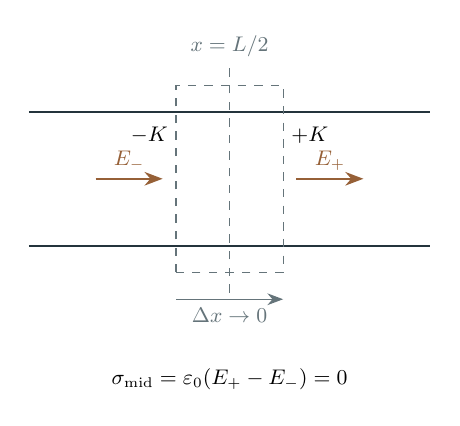
\begin{tikzpicture}[scale=.85,transform shape]

\draw[object] (-3,-1)--(3,-1);\draw[object] (-3,1)--(3,1);
\draw[guide] (0,-1.7)--(0,1.7) node[above] {$x=L/2$};
\draw[guide] (-.8,-1.4) rectangle (.8,1.4);
\draw[force] (-2,0)--(-1,0) node[midway,above] {$E_-$};
\draw[force] (1,0)--(2,0) node[midway,above] {$E_+$};
\draw[axis] (-.8,-1.8)--(.8,-1.8) node[midway,below] {$\Delta x\to0$};
\node at (0,-3) {$\sigma_{\rm mid}=\varepsilon_0(E_+-E_-)=0$};
\node[left] at (-.8,.65) {$-K$};\node[right] at (.8,.65) {$+K$};

\end{tikzpicture}
\figcaption{解图电试4.1B\quad 薄柱净通量由两侧场值差给出，有界体电荷在薄层内积分。}
\end{minipage}\end{center}
先让$h\to0$，体电荷在两侧有界，其总量的绝对值至多随$S_gh$趋零；截面若有有限面电荷，其总量则为$\sigma_{\rm mid}S_g$。高斯定律因此给
\[
\sigma_{\rm mid}=\varepsilon_0\bigl[E_x(L/2+0)-E_x(L/2-0)\bigr]
=\boxed{0}.
\]
两侧场值都趋于零，通量差随厚度趋零；两侧斜率分别给出有界的负、正体电荷。连续场的一阶分布导数只含上述有界体电荷，截面上没有额外的$\delta$项。

沿轴积分电场可得电势降，并把局部场与端电压联系起来。取$V(0)$为参考，$V(x)-V(0)=-\int_0^xE_x(\xi)\mathrm d\xi$。前半段直接积分正弦，
\[
V(x)=V(0)-\frac U4[1-\cos(2\pi x/L)],
\]
在中点先累积电势降$U/2$，再对后半段负正弦继续积分，得到
\[
V(x)=V(0)-\frac{3U}{4}-\frac U4\cos(2\pi x/L).
\]
\begin{center}\begin{minipage}{.98\linewidth}\centering
\begin{tikzpicture}[scale=.8,transform shape]
\draw[axis] (0,0)--(10.7,0) node[right] {$x/L$};
\draw[axis] (0,0)--(0,3.2) node[above] {$[V(0)-V(x)]/U$};\foreach \y/\lab in {0/0,1.4/0.5,2.8/1}{\draw[thin] (0,\y)--(-.08,\y) node[left] {$\lab$};}
\node[above] at (5,3.5) {电势降的累积量单调上升，中点为$1/2$};
\draw[traj] plot coordinates {(0.000000000,0.000000000) (0.083333333,0.000959326) (0.166666667,0.003834673) (0.250000000,0.008618162) (0.333333333,0.015296679) (0.416666667,0.023851922) (0.500000000,0.034260439) (0.583333333,0.046493701) (0.666666667,0.060518180) (0.750000000,0.076295433) (0.833333333,0.093782217) (0.916666667,0.112930602) (1.000000000,0.133688104) (1.083333333,0.155997827) (1.166666667,0.179798622) (1.250000000,0.205025253) (1.333333333,0.231608576) (1.416666667,0.259475726) (1.500000000,0.288550323) (1.583333333,0.318752675) (1.666666667,0.350000000) (1.750000000,0.382206650) (1.833333333,0.415284350) (1.916666667,0.449142435) (2.000000000,0.483688104) (2.083333333,0.518826668) (2.166666667,0.554461816) (2.250000000,0.590495874) (2.333333333,0.626830076) (2.416666667,0.663364831) (2.500000000,0.700000000) (2.583333333,0.736635169) (2.666666667,0.773169924) (2.750000000,0.809504126) (2.833333333,0.845538184) (2.916666667,0.881173332) (3.000000000,0.916311896) (3.083333333,0.950857565) (3.166666667,0.984715650) (3.250000000,1.017793350) (3.333333333,1.050000000) (3.416666667,1.081247325) (3.500000000,1.111449677) (3.583333333,1.140524274) (3.666666667,1.168391424) (3.750000000,1.194974747) (3.833333333,1.220201378) (3.916666667,1.244002173) (4.000000000,1.266311896) (4.083333333,1.287069398) (4.166666667,1.306217783) (4.250000000,1.323704567) (4.333333333,1.339481820) (4.416666667,1.353506299) (4.500000000,1.365739561) (4.583333333,1.376148078) (4.666666667,1.384703321) (4.750000000,1.391381838) (4.833333333,1.396165327) (4.916666667,1.399040674) (5.000000000,1.400000000) (5.083333333,1.400959326) (5.166666667,1.403834673) (5.250000000,1.408618162) (5.333333333,1.415296679) (5.416666667,1.423851922) (5.500000000,1.434260439) (5.583333333,1.446493701) (5.666666667,1.460518180) (5.750000000,1.476295433) (5.833333333,1.493782217) (5.916666667,1.512930602) (6.000000000,1.533688104) (6.083333333,1.555997827) (6.166666667,1.579798622) (6.250000000,1.605025253) (6.333333333,1.631608576) (6.416666667,1.659475726) (6.500000000,1.688550323) (6.583333333,1.718752675) (6.666666667,1.750000000) (6.750000000,1.782206650) (6.833333333,1.815284350) (6.916666667,1.849142435) (7.000000000,1.883688104) (7.083333333,1.918826668) (7.166666667,1.954461816) (7.250000000,1.990495874) (7.333333333,2.026830076) (7.416666667,2.063364831) (7.500000000,2.100000000) (7.583333333,2.136635169) (7.666666667,2.173169924) (7.750000000,2.209504126) (7.833333333,2.245538184) (7.916666667,2.281173332) (8.000000000,2.316311896) (8.083333333,2.350857565) (8.166666667,2.384715650) (8.250000000,2.417793350) (8.333333333,2.450000000) (8.416666667,2.481247325) (8.500000000,2.511449677) (8.583333333,2.540524274) (8.666666667,2.568391424) (8.750000000,2.594974747) (8.833333333,2.620201378) (8.916666667,2.644002173) (9.000000000,2.666311896) (9.083333333,2.687069398) (9.166666667,2.706217783) (9.250000000,2.723704567) (9.333333333,2.739481820) (9.416666667,2.753506299) (9.500000000,2.765739561) (9.583333333,2.776148078) (9.666666667,2.784703321) (9.750000000,2.791381838) (9.833333333,2.796165327) (9.916666667,2.799040674) (10.000000000,2.800000000)};
\node[below] at (0,-.12) {$0$};
\node[below] at (5,-.12) {$1/2$};
\node[below] at (10,-.12) {$1$};
\end{tikzpicture}
\figcaption{解图电试4.1C\quad 电势降的累积量单调上升，中点为$1/2$}
\end{minipage}\end{center}
解图电试4.1C画累计电势降$[V(0)-V(x)]/U$，中点为$1/2$，右端为1。电势连续下降，在场强为零的中点处斜率也为零。两段表达式在中点都给$V(0)-U/2$，右端给$V(L)=V(0)-U$。每半段的净体电荷为$\varepsilon_0S[E_x(x_{\rm right})-E_x(x_{\rm left})]=0$，与四段正负分布相容。两外端面的面电荷分别需要导体外侧的场值，端电压只给出内部场的积分。



\Needspace{8\baselineskip}

\pdfbookmark[3]{关键洞察}{q1-h5}

\subsection*{关键洞察}

中点两侧的体电荷从负值变为正值，描述的是场强曲线的斜率变化。场强本身连续且都趋于零，薄柱的极限通量为零，截面电荷也为零。非均匀体电荷正是维持非均匀局部场所需的稳恒分布，电流由这个场在各段共同驱动。每半段首尾电场同为零，所以半段内正负体电荷总量抵消。

\Needspace{8\baselineskip}

\pdfbookmark[3]{易错点}{q1-h6}

\subsection*{易错点}

电阻率取绝对值后，各微元电阻为非负，两半波积分相加。固定的是$j$，局部场$E_x$随$\rho$变化；平均场$U/L$只描述全长平均。后半段的绝对值为负正弦，求导时保留该负号。中点普通导数分别取左右值，截面面电荷则使用场值差；外端面电荷还需要导体外侧场值。

\Needspace{8\baselineskip}

\pdfbookmark[3]{课堂讲解建议}{q1-h7}

\subsection*{课堂讲解建议}

先画两个半波，让学生按曲线的上升、下降预测四个区间的电荷正负，再由欧姆定律和高斯定律求出幅值。要求把串联电阻积分、电场电压积分各写一次，说明相同电流如何与局部场变化相容。

在中点同时写$E_-=E_+=0$与$\rho_{e,-}=-K,\rho_{e,+}=K$。取薄柱并分别计算两端通量与层内有界体电荷，说明场值连续时截面电荷为零。最后由图C解释电势持续下降而中点瞬时斜率为零，并讨论外端面电荷所需的外部电场条件。

\Needspace{8\baselineskip}

\pdfbookmark[3]{变式训练}{q1-h8}

\subsection*{变式训练}

\begin{enumerate}
\Needspace{20\baselineskip}
\item 电阻率改为$\rho_0(1+x/L)$，求总电阻、内部电场和体电荷。
\textbf{解：}变图电试4.1V1中等截面微元串联，$R=\rho_0\int_0^L(1+x/L)\mathrm dx/S=3\rho_0L/(2S)$，所以$j=2U/(3\rho_0L)$。电场$E_x=2U(1+x/L)/(3L)$随轴向线性增加，其导数恒为$2U/(3L^2)$。因此$\rho_e=2\varepsilon_0U/(3L^2)>0$。内部场连续，无额外内部截面电荷；全段体电荷为$2\varepsilon_0US/(3L)$，相应两端场差满足高斯定律。
\begin{center}\begin{minipage}{.98\linewidth}\centering
\begin{tikzpicture}[scale=.8,transform shape]
\draw[axis] (0,0)--(10.7,0) node[right] {$x/L$};
\draw[axis] (0,0)--(0,3.2) node[above] {$E_xL/U$};\foreach \y/\lab in {0/0,1.1/0.5,2.2/1}{\draw[thin] (0,\y)--(-.08,\y) node[left] {$\lab$};}
\node[above] at (5,3.5) {线性电阻率给线性场和常量正体电荷};
\draw[traj] plot coordinates {(0.000000000,1.466666667) (0.083333333,1.478888889) (0.166666667,1.491111111) (0.250000000,1.503333333) (0.333333333,1.515555556) (0.416666667,1.527777778) (0.500000000,1.540000000) (0.583333333,1.552222222) (0.666666667,1.564444444) (0.750000000,1.576666667) (0.833333333,1.588888889) (0.916666667,1.601111111) (1.000000000,1.613333333) (1.083333333,1.625555556) (1.166666667,1.637777778) (1.250000000,1.650000000) (1.333333333,1.662222222) (1.416666667,1.674444444) (1.500000000,1.686666667) (1.583333333,1.698888889) (1.666666667,1.711111111) (1.750000000,1.723333333) (1.833333333,1.735555556) (1.916666667,1.747777778) (2.000000000,1.760000000) (2.083333333,1.772222222) (2.166666667,1.784444444) (2.250000000,1.796666667) (2.333333333,1.808888889) (2.416666667,1.821111111) (2.500000000,1.833333333) (2.583333333,1.845555556) (2.666666667,1.857777778) (2.750000000,1.870000000) (2.833333333,1.882222222) (2.916666667,1.894444444) (3.000000000,1.906666667) (3.083333333,1.918888889) (3.166666667,1.931111111) (3.250000000,1.943333333) (3.333333333,1.955555556) (3.416666667,1.967777778) (3.500000000,1.980000000) (3.583333333,1.992222222) (3.666666667,2.004444444) (3.750000000,2.016666667) (3.833333333,2.028888889) (3.916666667,2.041111111) (4.000000000,2.053333333) (4.083333333,2.065555556) (4.166666667,2.077777778) (4.250000000,2.090000000) (4.333333333,2.102222222) (4.416666667,2.114444444) (4.500000000,2.126666667) (4.583333333,2.138888889) (4.666666667,2.151111111) (4.750000000,2.163333333) (4.833333333,2.175555556) (4.916666667,2.187777778) (5.000000000,2.200000000) (5.083333333,2.212222222) (5.166666667,2.224444444) (5.250000000,2.236666667) (5.333333333,2.248888889) (5.416666667,2.261111111) (5.500000000,2.273333333) (5.583333333,2.285555556) (5.666666667,2.297777778) (5.750000000,2.310000000) (5.833333333,2.322222222) (5.916666667,2.334444444) (6.000000000,2.346666667) (6.083333333,2.358888889) (6.166666667,2.371111111) (6.250000000,2.383333333) (6.333333333,2.395555556) (6.416666667,2.407777778) (6.500000000,2.420000000) (6.583333333,2.432222222) (6.666666667,2.444444444) (6.750000000,2.456666667) (6.833333333,2.468888889) (6.916666667,2.481111111) (7.000000000,2.493333333) (7.083333333,2.505555556) (7.166666667,2.517777778) (7.250000000,2.530000000) (7.333333333,2.542222222) (7.416666667,2.554444444) (7.500000000,2.566666667) (7.583333333,2.578888889) (7.666666667,2.591111111) (7.750000000,2.603333333) (7.833333333,2.615555556) (7.916666667,2.627777778) (8.000000000,2.640000000) (8.083333333,2.652222222) (8.166666667,2.664444444) (8.250000000,2.676666667) (8.333333333,2.688888889) (8.416666667,2.701111111) (8.500000000,2.713333333) (8.583333333,2.725555556) (8.666666667,2.737777778) (8.750000000,2.750000000) (8.833333333,2.762222222) (8.916666667,2.774444444) (9.000000000,2.786666667) (9.083333333,2.798888889) (9.166666667,2.811111111) (9.250000000,2.823333333) (9.333333333,2.835555556) (9.416666667,2.847777778) (9.500000000,2.860000000) (9.583333333,2.872222222) (9.666666667,2.884444444) (9.750000000,2.896666667) (9.833333333,2.908888889) (9.916666667,2.921111111) (10.000000000,2.933333333)};
\node[below] at (0,-.12) {$0$};
\node[below] at (5,-.12) {$1/2$};
\node[below] at (10,-.12) {$1$};
\end{tikzpicture}
\figcaption{变图电试4.1V1\quad 线性电阻率给线性场和常量正体电荷}
\end{minipage}\end{center}

\Needspace{20\baselineskip}
\item 两段常电阻率$\rho_a,\rho_b$串联，长度分别为$L_a,L_b$，截面仍为$S$。求体电荷和接面电荷。
\textbf{解：}变图电试4.1V2令接面法向从$a$指向$b$。总电阻$(\rho_aL_a+\rho_bL_b)/S$，故$j=U/(\rho_aL_a+\rho_bL_b)$。两段内场分别为$E_a=\rho_aj,E_b=\rho_bj$，各自常量使内部体电荷为零。跨接面高斯薄柱给$\sigma=\varepsilon_0(E_b-E_a)=\varepsilon_0j(\rho_b-\rho_a)$，$\rho_b>\rho_a$时接面带正电。场的有限跳跃在这里直接对应一层面电荷。
\begin{center}\begin{minipage}{.98\linewidth}\centering
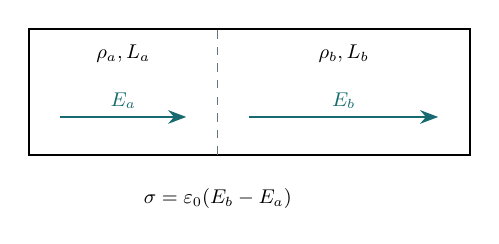
\begin{tikzpicture}[scale=.8,transform shape]
\draw[thick] (0,0) rectangle (7,2);\draw[guide] (3,0)--(3,2);\node at (1.5,1.6) {$\rho_a,L_a$};\node at (5,1.6) {$\rho_b,L_b$};\draw[motion] (.5,.6)--(2.5,.6) node[midway,above] {$E_a$};\draw[motion] (3.5,.6)--(6.5,.6) node[midway,above] {$E_b$};\node at (3,-.7) {$\sigma=\varepsilon_0(E_b-E_a)$};
\end{tikzpicture}
\figcaption{变图电试4.1V2\quad 两段常电阻率连接处，面电荷由轴向场的有限跳变给出}
\end{minipage}\end{center}

\Needspace{20\baselineskip}
\item 电阻率改为$\rho_0\sin^2(2\pi x/L)$，求电阻、电场与体电荷并讨论中点。
\textbf{解：}变图电试4.1V3的平方正弦平均为$1/2$，$R=\rho_0L/(2S)$、$j=2U/(\rho_0L)$。场强$E_x=2U\sin^2(2\pi x/L)/L$，求导用$2\sin a\cos a=\sin2a$，得$\rho_e=4\pi\varepsilon_0U\sin(4\pi x/L)/L^2$。中点场值与导数都连续且为零，所以该截面面电荷为零。正电区仍为第一和第三个四分之一区间，但电荷曲线在中点平滑过零。
\begin{center}\begin{minipage}{.98\linewidth}\centering
\begin{tikzpicture}[scale=.8,transform shape]
\draw[axis] (0,0)--(10.7,0) node[right] {$x/L$};
\draw[axis] (0,0)--(0,3.2) node[above] {$E_xL/U$};\foreach \y/\lab in {0/0,1.4/1,2.8/2}{\draw[thin] (0,\y)--(-.08,\y) node[left] {$\lab$};}
\node[above] at (5,3.5) {平方正弦电场在中点光滑，体电荷连续过零};
\draw[traj] plot coordinates {(0.000000000,0.000000000) (0.083333333,0.007669346) (0.166666667,0.030593359) (0.250000000,0.068520877) (0.333333333,0.121036359) (0.416666667,0.187564435) (0.500000000,0.267376208) (0.583333333,0.359597244) (0.666666667,0.463217151) (0.750000000,0.577100647) (0.833333333,0.700000000) (0.916666667,0.830568700) (1.000000000,0.967376208) (1.083333333,1.108923633) (1.166666667,1.253660151) (1.250000000,1.400000000) (1.333333333,1.546339849) (1.416666667,1.691076367) (1.500000000,1.832623792) (1.583333333,1.969431300) (1.666666667,2.100000000) (1.750000000,2.222899353) (1.833333333,2.336782849) (1.916666667,2.440402756) (2.000000000,2.532623792) (2.083333333,2.612435565) (2.166666667,2.678963641) (2.250000000,2.731479123) (2.333333333,2.769406641) (2.416666667,2.792330654) (2.500000000,2.800000000) (2.583333333,2.792330654) (2.666666667,2.769406641) (2.750000000,2.731479123) (2.833333333,2.678963641) (2.916666667,2.612435565) (3.000000000,2.532623792) (3.083333333,2.440402756) (3.166666667,2.336782849) (3.250000000,2.222899353) (3.333333333,2.100000000) (3.416666667,1.969431300) (3.500000000,1.832623792) (3.583333333,1.691076367) (3.666666667,1.546339849) (3.750000000,1.400000000) (3.833333333,1.253660151) (3.916666667,1.108923633) (4.000000000,0.967376208) (4.083333333,0.830568700) (4.166666667,0.700000000) (4.250000000,0.577100647) (4.333333333,0.463217151) (4.416666667,0.359597244) (4.500000000,0.267376208) (4.583333333,0.187564435) (4.666666667,0.121036359) (4.750000000,0.068520877) (4.833333333,0.030593359) (4.916666667,0.007669346) (5.000000000,0.000000000) (5.083333333,0.007669346) (5.166666667,0.030593359) (5.250000000,0.068520877) (5.333333333,0.121036359) (5.416666667,0.187564435) (5.500000000,0.267376208) (5.583333333,0.359597244) (5.666666667,0.463217151) (5.750000000,0.577100647) (5.833333333,0.700000000) (5.916666667,0.830568700) (6.000000000,0.967376208) (6.083333333,1.108923633) (6.166666667,1.253660151) (6.250000000,1.400000000) (6.333333333,1.546339849) (6.416666667,1.691076367) (6.500000000,1.832623792) (6.583333333,1.969431300) (6.666666667,2.100000000) (6.750000000,2.222899353) (6.833333333,2.336782849) (6.916666667,2.440402756) (7.000000000,2.532623792) (7.083333333,2.612435565) (7.166666667,2.678963641) (7.250000000,2.731479123) (7.333333333,2.769406641) (7.416666667,2.792330654) (7.500000000,2.800000000) (7.583333333,2.792330654) (7.666666667,2.769406641) (7.750000000,2.731479123) (7.833333333,2.678963641) (7.916666667,2.612435565) (8.000000000,2.532623792) (8.083333333,2.440402756) (8.166666667,2.336782849) (8.250000000,2.222899353) (8.333333333,2.100000000) (8.416666667,1.969431300) (8.500000000,1.832623792) (8.583333333,1.691076367) (8.666666667,1.546339849) (8.750000000,1.400000000) (8.833333333,1.253660151) (8.916666667,1.108923633) (9.000000000,0.967376208) (9.083333333,0.830568700) (9.166666667,0.700000000) (9.250000000,0.577100647) (9.333333333,0.463217151) (9.416666667,0.359597244) (9.500000000,0.267376208) (9.583333333,0.187564435) (9.666666667,0.121036359) (9.750000000,0.068520877) (9.833333333,0.030593359) (9.916666667,0.007669346) (10.000000000,0.000000000)};
\node[below] at (0,-.12) {$0$};
\node[below] at (5,-.12) {$1/2$};
\node[below] at (10,-.12) {$1$};
\end{tikzpicture}
\figcaption{变图电试4.1V3\quad 平方正弦电场在中点光滑，体电荷连续过零}
\end{minipage}\end{center}

\Needspace{20\baselineskip}
\item 全部电阻率统一乘$c>0$，分别在固定端电压和固定总电流下讨论场及体电荷。
\textbf{解：}变图电试4.1V4中串联积分给$R\to cR$。固定$U$时$I,j$都除以$c$，所以$E_x=(c\rho)(j/c)=\rho j$，电场与其导数给出的$\rho_e$均保持相同。固定$I$时$j$不变，故$E_x$和$\rho_e$都乘$c$，端电压也乘$c$。相同材料比例变化对应何种电场响应，由外部电路保持的物理量决定。
\begin{center}\begin{minipage}{.98\linewidth}\centering
\begin{tikzpicture}[scale=.8,transform shape]
\node[draw] at (0,1) {$\rho\to c\rho$};\node[draw,align=center] at (4,2) {固定$U$：$j\to j/c$\quad $E,\rho_e$不变};\node[draw,align=center] at (4,0) {固定$I$：$j$不变\quad $E,\rho_e\to cE,c\rho_e$};\draw[axis] (1,1)--(2,2);\draw[axis] (1,1)--(2,0);
\end{tikzpicture}
\figcaption{变图电试4.1V4\quad 同一材料变化在两种外部控制条件下的响应}
\end{minipage}\end{center}

\Needspace{20\baselineskip}
\item 电阻率改为$\rho_b+\rho_0|\sin(2\pi x/L)|$，$\rho_b>0$，固定端电压$U$。求电阻和中点电荷情况。
\textbf{解：}变图电试4.1V5的常量部分和波形部分积分相加，$R=L(\rho_b+2\rho_0/\pi)/S$，$j=U/[L(\rho_b+2\rho_0/\pi)]$。场强为$j[\rho_b+\rho_0|\sin(2\pi x/L)|]$，体电荷在两半区分别为$\pm(2\pi\varepsilon_0j\rho_0/L)\cos(2\pi x/L)$。中点场值两侧同为$j\rho_b$，故面电荷仍为零。常量电阻率抬高场的最低值，并通过减小$j$降低体电荷幅值。
\begin{center}\begin{minipage}{.98\linewidth}\centering
\begin{tikzpicture}[scale=.8,transform shape]
\draw[axis] (0,0)--(10.7,0) node[right] {$x/L$};
\draw[axis] (0,0)--(0,3.2) node[above] {$E_xL/U$};\foreach \y/\lab in {0/0,0.9/0.5,1.8/1,2.7/1.5}{\draw[thin] (0,\y)--(-.08,\y) node[left] {$\lab$};}
\node[above] at (5,3.5) {实线无常量电阻率，虚线加$\rho_b=\rho_0$；积分均为1};
\draw[traj] plot coordinates {(0.000000000,0.000000000) (0.083333333,0.147976430) (0.166666667,0.295547267) (0.250000000,0.442308030) (0.333333333,0.587856456) (0.416666667,0.731793610) (0.500000000,0.873724967) (0.583333333,1.013261506) (0.666666667,1.150020765) (0.750000000,1.283627897) (0.833333333,1.413716694) (0.916666667,1.539930592) (1.000000000,1.661923647) (1.083333333,1.779361486) (1.166666667,1.891922218) (1.250000000,1.999297322) (1.333333333,2.101192492) (1.416666667,2.197328439) (1.500000000,2.287441662) (1.583333333,2.371285166) (1.666666667,2.448629142) (1.750000000,2.519261596) (1.833333333,2.582988929) (1.916666667,2.639636468) (2.000000000,2.689048948) (2.083333333,2.731090932) (2.166666667,2.765647185) (2.250000000,2.792622991) (2.333333333,2.811944412) (2.416666667,2.823558489) (2.500000000,2.827433388) (2.583333333,2.823558489) (2.666666667,2.811944412) (2.750000000,2.792622991) (2.833333333,2.765647185) (2.916666667,2.731090932) (3.000000000,2.689048948) (3.083333333,2.639636468) (3.166666667,2.582988929) (3.250000000,2.519261596) (3.333333333,2.448629142) (3.416666667,2.371285166) (3.500000000,2.287441662) (3.583333333,2.197328439) (3.666666667,2.101192492) (3.750000000,1.999297322) (3.833333333,1.891922218) (3.916666667,1.779361486) (4.000000000,1.661923647) (4.083333333,1.539930592) (4.166666667,1.413716694) (4.250000000,1.283627897) (4.333333333,1.150020765) (4.416666667,1.013261506) (4.500000000,0.873724967) (4.583333333,0.731793610) (4.666666667,0.587856456) (4.750000000,0.442308030) (4.833333333,0.295547267) (4.916666667,0.147976430) (5.000000000,0.000000000) (5.083333333,0.147976430) (5.166666667,0.295547267) (5.250000000,0.442308030) (5.333333333,0.587856456) (5.416666667,0.731793610) (5.500000000,0.873724967) (5.583333333,1.013261506) (5.666666667,1.150020765) (5.750000000,1.283627897) (5.833333333,1.413716694) (5.916666667,1.539930592) (6.000000000,1.661923647) (6.083333333,1.779361486) (6.166666667,1.891922218) (6.250000000,1.999297322) (6.333333333,2.101192492) (6.416666667,2.197328439) (6.500000000,2.287441662) (6.583333333,2.371285166) (6.666666667,2.448629142) (6.750000000,2.519261596) (6.833333333,2.582988929) (6.916666667,2.639636468) (7.000000000,2.689048948) (7.083333333,2.731090932) (7.166666667,2.765647185) (7.250000000,2.792622991) (7.333333333,2.811944412) (7.416666667,2.823558489) (7.500000000,2.827433388) (7.583333333,2.823558489) (7.666666667,2.811944412) (7.750000000,2.792622991) (7.833333333,2.765647185) (7.916666667,2.731090932) (8.000000000,2.689048948) (8.083333333,2.639636468) (8.166666667,2.582988929) (8.250000000,2.519261596) (8.333333333,2.448629142) (8.416666667,2.371285166) (8.500000000,2.287441662) (8.583333333,2.197328439) (8.666666667,2.101192492) (8.750000000,1.999297322) (8.833333333,1.891922218) (8.916666667,1.779361486) (9.000000000,1.661923647) (9.083333333,1.539930592) (9.166666667,1.413716694) (9.250000000,1.283627897) (9.333333333,1.150020765) (9.416666667,1.013261506) (9.500000000,0.873724967) (9.583333333,0.731793610) (9.666666667,0.587856456) (9.750000000,0.442308030) (9.833333333,0.295547267) (9.916666667,0.147976430) (10.000000000,0.000000000)};
\draw[dashed,thick,color=warm] plot coordinates {(0.000000000,1.099827847) (0.083333333,1.157388389) (0.166666667,1.214791161) (0.250000000,1.271878827) (0.333333333,1.328494914) (0.416666667,1.384484240) (0.500000000,1.439693342) (0.583333333,1.493970897) (0.666666667,1.547168133) (0.750000000,1.599139240) (0.833333333,1.649741770) (0.916666667,1.698837024) (1.000000000,1.746290435) (1.083333333,1.791971937) (1.166666667,1.835756321) (1.250000000,1.877523575) (1.333333333,1.917159220) (1.416666667,1.954554616) (1.500000000,1.989607265) (1.583333333,2.022221091) (1.666666667,2.052306702) (1.750000000,2.079781633) (1.833333333,2.104570580) (1.916666667,2.126605597) (2.000000000,2.145826287) (2.083333333,2.162179968) (2.166666667,2.175621816) (2.250000000,2.186114987) (2.333333333,2.193630721) (2.416666667,2.198148417) (2.500000000,2.199655693) (2.583333333,2.198148417) (2.666666667,2.193630721) (2.750000000,2.186114987) (2.833333333,2.175621816) (2.916666667,2.162179968) (3.000000000,2.145826287) (3.083333333,2.126605597) (3.166666667,2.104570580) (3.250000000,2.079781633) (3.333333333,2.052306702) (3.416666667,2.022221091) (3.500000000,1.989607265) (3.583333333,1.954554616) (3.666666667,1.917159220) (3.750000000,1.877523575) (3.833333333,1.835756321) (3.916666667,1.791971937) (4.000000000,1.746290435) (4.083333333,1.698837024) (4.166666667,1.649741770) (4.250000000,1.599139240) (4.333333333,1.547168133) (4.416666667,1.493970897) (4.500000000,1.439693342) (4.583333333,1.384484240) (4.666666667,1.328494914) (4.750000000,1.271878827) (4.833333333,1.214791161) (4.916666667,1.157388389) (5.000000000,1.099827847) (5.083333333,1.157388389) (5.166666667,1.214791161) (5.250000000,1.271878827) (5.333333333,1.328494914) (5.416666667,1.384484240) (5.500000000,1.439693342) (5.583333333,1.493970897) (5.666666667,1.547168133) (5.750000000,1.599139240) (5.833333333,1.649741770) (5.916666667,1.698837024) (6.000000000,1.746290435) (6.083333333,1.791971937) (6.166666667,1.835756321) (6.250000000,1.877523575) (6.333333333,1.917159220) (6.416666667,1.954554616) (6.500000000,1.989607265) (6.583333333,2.022221091) (6.666666667,2.052306702) (6.750000000,2.079781633) (6.833333333,2.104570580) (6.916666667,2.126605597) (7.000000000,2.145826287) (7.083333333,2.162179968) (7.166666667,2.175621816) (7.250000000,2.186114987) (7.333333333,2.193630721) (7.416666667,2.198148417) (7.500000000,2.199655693) (7.583333333,2.198148417) (7.666666667,2.193630721) (7.750000000,2.186114987) (7.833333333,2.175621816) (7.916666667,2.162179968) (8.000000000,2.145826287) (8.083333333,2.126605597) (8.166666667,2.104570580) (8.250000000,2.079781633) (8.333333333,2.052306702) (8.416666667,2.022221091) (8.500000000,1.989607265) (8.583333333,1.954554616) (8.666666667,1.917159220) (8.750000000,1.877523575) (8.833333333,1.835756321) (8.916666667,1.791971937) (9.000000000,1.746290435) (9.083333333,1.698837024) (9.166666667,1.649741770) (9.250000000,1.599139240) (9.333333333,1.547168133) (9.416666667,1.493970897) (9.500000000,1.439693342) (9.583333333,1.384484240) (9.666666667,1.328494914) (9.750000000,1.271878827) (9.833333333,1.214791161) (9.916666667,1.157388389) (10.000000000,1.099827847)};
\node[below] at (0,-.12) {$0$};
\node[below] at (5,-.12) {$1/2$};
\node[below] at (10,-.12) {$1$};
\end{tikzpicture}
\figcaption{变图电试4.1V5\quad 实线无常量电阻率，虚线加$\rho_b=\rho_0$；积分均为1}
\end{minipage}\end{center}

\Needspace{20\baselineskip}
\item 求题设导体单位体积的焦耳热功率和轴向累积耗散，说明哪处发热最强。
\textbf{解：}变图电试4.1V6中$p_v=jE_x=j^2\rho_0|\sin(2\pi x/L)|$，在$x=L/4,3L/4$最大，在端点及中点为零。全导体积分$P=S\int_0^LjE_x\mathrm dx=I\int_0^LE_x\mathrm dx=IU=U^2/R$。到位置$x$为止耗散的比例为$P(0,x)/P=\int_0^xE_x\mathrm dx/U=[V(0)-V(x)]/U$，由电势降曲线直接读出。发热密度与场值同形，体电荷则与场的斜率同形，各自对应不同物理关系。
\begin{center}\begin{minipage}{.98\linewidth}\centering
\begin{tikzpicture}[scale=.8,transform shape]
\draw[axis] (0,0)--(10.7,0) node[right] {$x/L$};
\draw[axis] (0,0)--(0,3.2) node[above] {$[V(0)-V(x)]/U$};\foreach \y/\lab in {0/0,1.4/0.5,2.8/1}{\draw[thin] (0,\y)--(-.08,\y) node[left] {$\lab$};}
\node[above] at (5,3.5) {电势降的累积量单调上升，中点为$1/2$};
\draw[traj] plot coordinates {(0.000000000,0.000000000) (0.083333333,0.000959326) (0.166666667,0.003834673) (0.250000000,0.008618162) (0.333333333,0.015296679) (0.416666667,0.023851922) (0.500000000,0.034260439) (0.583333333,0.046493701) (0.666666667,0.060518180) (0.750000000,0.076295433) (0.833333333,0.093782217) (0.916666667,0.112930602) (1.000000000,0.133688104) (1.083333333,0.155997827) (1.166666667,0.179798622) (1.250000000,0.205025253) (1.333333333,0.231608576) (1.416666667,0.259475726) (1.500000000,0.288550323) (1.583333333,0.318752675) (1.666666667,0.350000000) (1.750000000,0.382206650) (1.833333333,0.415284350) (1.916666667,0.449142435) (2.000000000,0.483688104) (2.083333333,0.518826668) (2.166666667,0.554461816) (2.250000000,0.590495874) (2.333333333,0.626830076) (2.416666667,0.663364831) (2.500000000,0.700000000) (2.583333333,0.736635169) (2.666666667,0.773169924) (2.750000000,0.809504126) (2.833333333,0.845538184) (2.916666667,0.881173332) (3.000000000,0.916311896) (3.083333333,0.950857565) (3.166666667,0.984715650) (3.250000000,1.017793350) (3.333333333,1.050000000) (3.416666667,1.081247325) (3.500000000,1.111449677) (3.583333333,1.140524274) (3.666666667,1.168391424) (3.750000000,1.194974747) (3.833333333,1.220201378) (3.916666667,1.244002173) (4.000000000,1.266311896) (4.083333333,1.287069398) (4.166666667,1.306217783) (4.250000000,1.323704567) (4.333333333,1.339481820) (4.416666667,1.353506299) (4.500000000,1.365739561) (4.583333333,1.376148078) (4.666666667,1.384703321) (4.750000000,1.391381838) (4.833333333,1.396165327) (4.916666667,1.399040674) (5.000000000,1.400000000) (5.083333333,1.400959326) (5.166666667,1.403834673) (5.250000000,1.408618162) (5.333333333,1.415296679) (5.416666667,1.423851922) (5.500000000,1.434260439) (5.583333333,1.446493701) (5.666666667,1.460518180) (5.750000000,1.476295433) (5.833333333,1.493782217) (5.916666667,1.512930602) (6.000000000,1.533688104) (6.083333333,1.555997827) (6.166666667,1.579798622) (6.250000000,1.605025253) (6.333333333,1.631608576) (6.416666667,1.659475726) (6.500000000,1.688550323) (6.583333333,1.718752675) (6.666666667,1.750000000) (6.750000000,1.782206650) (6.833333333,1.815284350) (6.916666667,1.849142435) (7.000000000,1.883688104) (7.083333333,1.918826668) (7.166666667,1.954461816) (7.250000000,1.990495874) (7.333333333,2.026830076) (7.416666667,2.063364831) (7.500000000,2.100000000) (7.583333333,2.136635169) (7.666666667,2.173169924) (7.750000000,2.209504126) (7.833333333,2.245538184) (7.916666667,2.281173332) (8.000000000,2.316311896) (8.083333333,2.350857565) (8.166666667,2.384715650) (8.250000000,2.417793350) (8.333333333,2.450000000) (8.416666667,2.481247325) (8.500000000,2.511449677) (8.583333333,2.540524274) (8.666666667,2.568391424) (8.750000000,2.594974747) (8.833333333,2.620201378) (8.916666667,2.644002173) (9.000000000,2.666311896) (9.083333333,2.687069398) (9.166666667,2.706217783) (9.250000000,2.723704567) (9.333333333,2.739481820) (9.416666667,2.753506299) (9.500000000,2.765739561) (9.583333333,2.776148078) (9.666666667,2.784703321) (9.750000000,2.791381838) (9.833333333,2.796165327) (9.916666667,2.799040674) (10.000000000,2.800000000)};
\node[below] at (0,-.12) {$0$};
\node[below] at (5,-.12) {$1/2$};
\node[below] at (10,-.12) {$1$};
\end{tikzpicture}
\figcaption{变图电试4.1V6\quad 电势降的累积量单调上升，中点为$1/2$}
\end{minipage}\end{center}

\Needspace{20\baselineskip}
\item 求题设每个四分之一区段的净体电荷，以及整个内部体电荷相对$x=0$的轴向偶极矩。
\textbf{解：}变图电试4.1V7用高斯定律积分，任一区段$[a,b]$的体电荷为$\varepsilon_0S[E_x(b)-E_x(a)]$。场峰值$E_m=\pi U/(2L)$，故四段电荷依次为$+\varepsilon_0SE_m,-\varepsilon_0SE_m,+\varepsilon_0SE_m,-\varepsilon_0SE_m$，总量为零。轴向偶极矩$p_x=S\int_0^Lx\rho_e\mathrm dx=\varepsilon_0S[xE_x]_0^L-\varepsilon_0S\int_0^LE_x\mathrm dx=-\varepsilon_0SU$。端点场为零且总电荷为零，偶极矩与坐标原点的平移无关，方向沿$-x$。
\begin{center}\begin{minipage}{.98\linewidth}\centering
\begin{tikzpicture}[scale=.8,transform shape]
\draw[axis] (0,0)--(8.5,0) node[right] {$x$};\foreach \x/\lab in {1/+,3/-,5/+,7/-}{\node[draw,circle] at (\x,1) {$\lab$};}\draw[guide] (2,-.4)--(2,1.6);\draw[guide] (4,-.4)--(4,1.6);\draw[guide] (6,-.4)--(6,1.6);\node at (4,2.4) {四段净电荷大小均为$\varepsilon_0S\pi U/(2L)$};\draw[motion] (5,-1)--(3,-1) node[midway,below] {$p_x=-\varepsilon_0SU$};
\end{tikzpicture}
\figcaption{变图电试4.1V7\quad 四分之一区段的净电荷与内部电荷偶极矩}
\end{minipage}\end{center}

\Needspace{20\baselineskip}
\item 电阻率改为三角形分布：前半段$2\rho_0x/L$，后半段$2\rho_0(1-x/L)$。求电场、体电荷及中点面电荷。
\textbf{解：}变图电试4.1V8的电阻率积分为三角形面积$\rho_0L/2$，所以$R=\rho_0L/(2S)$、$j=2U/(\rho_0L)$。场强前半段为$4Ux/L^2$，后半段为$4U(1-x/L)/L$，中点两侧同为$2U/L$。体电荷前半段恒为$4\varepsilon_0U/L^2$，后半段恒为负的同值；它们的跃变对应场的斜率改变，中点面电荷仍由场值差给零。两半段的正负总电荷相消，电势降仍积分为$U$。
\begin{center}\begin{minipage}{.98\linewidth}\centering
\begin{tikzpicture}[scale=.8,transform shape]
\draw[axis] (0,0)--(10.7,0) node[right] {$x/L$};
\draw[axis] (0,0)--(0,3.2) node[above] {$E_xL/U$};\foreach \y/\lab in {0/0,1.4/1,2.8/2}{\draw[thin] (0,\y)--(-.08,\y) node[left] {$\lab$};}
\node[above] at (5,3.5) {三角形场连续，体电荷在中点由正常量变负常量};
\draw[traj] plot coordinates {(0.000000000,0.000000000) (0.083333333,0.046666667) (0.166666667,0.093333333) (0.250000000,0.140000000) (0.333333333,0.186666667) (0.416666667,0.233333333) (0.500000000,0.280000000) (0.583333333,0.326666667) (0.666666667,0.373333333) (0.750000000,0.420000000) (0.833333333,0.466666667) (0.916666667,0.513333333) (1.000000000,0.560000000) (1.083333333,0.606666667) (1.166666667,0.653333333) (1.250000000,0.700000000) (1.333333333,0.746666667) (1.416666667,0.793333333) (1.500000000,0.840000000) (1.583333333,0.886666667) (1.666666667,0.933333333) (1.750000000,0.980000000) (1.833333333,1.026666667) (1.916666667,1.073333333) (2.000000000,1.120000000) (2.083333333,1.166666667) (2.166666667,1.213333333) (2.250000000,1.260000000) (2.333333333,1.306666667) (2.416666667,1.353333333) (2.500000000,1.400000000) (2.583333333,1.446666667) (2.666666667,1.493333333) (2.750000000,1.540000000) (2.833333333,1.586666667) (2.916666667,1.633333333) (3.000000000,1.680000000) (3.083333333,1.726666667) (3.166666667,1.773333333) (3.250000000,1.820000000) (3.333333333,1.866666667) (3.416666667,1.913333333) (3.500000000,1.960000000) (3.583333333,2.006666667) (3.666666667,2.053333333) (3.750000000,2.100000000) (3.833333333,2.146666667) (3.916666667,2.193333333) (4.000000000,2.240000000) (4.083333333,2.286666667) (4.166666667,2.333333333) (4.250000000,2.380000000) (4.333333333,2.426666667) (4.416666667,2.473333333) (4.500000000,2.520000000) (4.583333333,2.566666667) (4.666666667,2.613333333) (4.750000000,2.660000000) (4.833333333,2.706666667) (4.916666667,2.753333333) (5.000000000,2.800000000) (5.083333333,2.753333333) (5.166666667,2.706666667) (5.250000000,2.660000000) (5.333333333,2.613333333) (5.416666667,2.566666667) (5.500000000,2.520000000) (5.583333333,2.473333333) (5.666666667,2.426666667) (5.750000000,2.380000000) (5.833333333,2.333333333) (5.916666667,2.286666667) (6.000000000,2.240000000) (6.083333333,2.193333333) (6.166666667,2.146666667) (6.250000000,2.100000000) (6.333333333,2.053333333) (6.416666667,2.006666667) (6.500000000,1.960000000) (6.583333333,1.913333333) (6.666666667,1.866666667) (6.750000000,1.820000000) (6.833333333,1.773333333) (6.916666667,1.726666667) (7.000000000,1.680000000) (7.083333333,1.633333333) (7.166666667,1.586666667) (7.250000000,1.540000000) (7.333333333,1.493333333) (7.416666667,1.446666667) (7.500000000,1.400000000) (7.583333333,1.353333333) (7.666666667,1.306666667) (7.750000000,1.260000000) (7.833333333,1.213333333) (7.916666667,1.166666667) (8.000000000,1.120000000) (8.083333333,1.073333333) (8.166666667,1.026666667) (8.250000000,0.980000000) (8.333333333,0.933333333) (8.416666667,0.886666667) (8.500000000,0.840000000) (8.583333333,0.793333333) (8.666666667,0.746666667) (8.750000000,0.700000000) (8.833333333,0.653333333) (8.916666667,0.606666667) (9.000000000,0.560000000) (9.083333333,0.513333333) (9.166666667,0.466666667) (9.250000000,0.420000000) (9.333333333,0.373333333) (9.416666667,0.326666667) (9.500000000,0.280000000) (9.583333333,0.233333333) (9.666666667,0.186666667) (9.750000000,0.140000000) (9.833333333,0.093333333) (9.916666667,0.046666667) (10.000000000,0.000000000)};
\node[below] at (0,-.12) {$0$};
\node[below] at (5,-.12) {$1/2$};
\node[below] at (10,-.12) {$1$};
\end{tikzpicture}
\figcaption{变图电试4.1V8\quad 三角形场连续，体电荷在中点由正常量变负常量}
\end{minipage}\end{center}
\end{enumerate}

\Needspace{13\baselineskip}

\pdfbookmark[2]{第 2 题 多端等效与无限内接三角形网络}{q2}

\section*{第 2 题\quad 多端等效与无限内接三角形网络}\label{q:2}


\begin{enumerate}
\item $N$端电阻网络可用外端两两之间的等效支路表示。说明这种表示中何时须允许开路支路，画出四端完全网络，以及一个由八个电阻组成、不能直接串并联约化的四端网络。
\item 等边三角形$ABC$的三边均被中点$P,Q,T$分为两段，每段电阻为$R$，三个中点之间也各接一个电阻$R$，其中$P$在$AB$、$Q$在$BC$、$T$在$CA$。求其对外端$A,B,C$的对称三角形等效网络。
\item 两个边长$a$的等边三角形$ABC$与$BCD$共边$BC$。左三角形中不断连接三边中点构成内接三角形，所有中点均电连接；右侧只增加$CD,DB$两段。各段为相同材料和粗细的金属丝，单位长度电阻$r$。求全网络$A,B$间等效电阻。
\end{enumerate}
无限网络按有限层截断、最内层不再加支路的极限定义。


\begin{center}\begin{minipage}{.98\linewidth}\centering
\begin{tikzpicture}[scale=.7,transform shape]

\coordinate (A) at (0,0);\coordinate (B) at (4,0);\coordinate (C) at (2,3.464);
\coordinate (P) at (2,0);\coordinate (Q) at (3,1.732);\coordinate (T) at (1,1.732);
\draw[object] (A)--(B)--(C)--cycle;\draw[object] (P)--(Q)--(T)--cycle;
\foreach \p/\pos in {A/below left,B/below right,C/above,P/below,Q/right,T/left}{\fill (\p) circle (1.6pt) node[\pos] {$\p$};}
\node at (2,-1) {每一小段均为$R$};\begin{scope}[xshift=7cm]
\coordinate (A) at (0,0);\coordinate (B) at (4,0);\coordinate (C) at (2,3.464);
\coordinate (D) at (6,3.464);
\draw[object] (A)--(B)--(C)--cycle;\draw[object] (C)--(D)--(B);
\foreach \k in {1,...,7}{
\coordinate (M) at ($(A)!.5!(B)$);\coordinate (N) at ($(B)!.5!(C)$);\coordinate (O) at ($(C)!.5!(A)$);
\draw[object] (M)--(N)--(O)--cycle;
\coordinate (A) at (M);\coordinate (B) at (N);\coordinate (C) at (O);}
\node[below left] at (0,0) {$A$};\node[below] at (4,0) {$B$};
\node[above] at (2,3.464) {$C$};\node[above right] at (6,3.464) {$D$};
\node[above] at (4,3.464) {$k=ar$};\node[right] at (5,1.732) {$k$};
\node at (3,-1) {左部无限内接，右部仅加两边};\end{scope}
\end{tikzpicture}
\figcaption{图电试4.2\quad 有限九电阻三角形与共边的无限三角形组合。}
\end{minipage}\end{center}

\Needspace{8\baselineskip}

\pdfbookmark[3]{题型定位}{q2-h0}

\subsection*{题型定位}

多端电阻网络的外端导纳等效、三重对称与无限层递推。外端整体等效由一组电流—电势关系表达，有限的对称三角形先示范怎样从两端测量确定三端等效，再用缩放网络与有限截断说明无限极限。相邻三角形的共边计入左部一次，右部再作为两条新增支路接入。

\Needspace{8\baselineskip}

\pdfbookmark[3]{知识点}{q2-h1}

\subsection*{知识点}

结点导纳矩阵和内部无注入电流条件给出Schur消元。正电阻网络的外端约化导纳行和为零，非对角元非正，零电导对应开路。三外端置换对称保证三条等效边相等，第三端开路时两端电阻是等效边的$2/3$。按线长缩放电阻形成递推；有限截断定义物理极限，导数界给误差控制。相同电势结点可在各自子网均守恒时分拆，新增被动通路降低端口电阻。

\Needspace{8\baselineskip}

\pdfbookmark[3]{物理图像}{q2-h2}

\subsection*{物理图像}

题图区分左部无限三角形、共边$BC$与右部新增两边。解图电试4.2A的四端完全图对角线交叉处无结点，八电阻图则有内部中心。图B保留$A,B$反对称激励下$C,P$为零、$T,Q$为相反电势的结构；图D把中点$P$分拆后，将两侧中点之间的小网标成二端电阻$X/2$。图E按同一开端截断给出有限层收敛。图C用等效三角形吸收整个左网后，只加右部$C-D-B$路径。

\Needspace{8\baselineskip}

\pdfbookmark[3]{解题入口}{q2-h3}

\subsection*{解题入口}

先在四端图逐一辨认外端与内部结点，说明外端保留为可独立接线的端点。有限题列六结点方程，解出一组电势，再由全置换对称确定三条等效边。无限题定义左网二端电阻$X$，先说明尺度与三端等效边的区别，再用反对称电势求递推；最后按有限截断起点选取正极限，并接回右部。

\Needspace{8\baselineskip}

\pdfbookmark[3]{标准解法}{q2-h4}

\subsection*{标准解法}


图电试4.2给出外端、内部结点及共边关系。多端等效要求对所有允许的外端电势给出相同的外端电流，仅匹配一次两端测量一般不足。

第（1）问，可把有限网络的结点导纳矩阵分成外端$b$与内部$i$两部分。内部无外注入电流，
\[
\begin{pmatrix}I_b\\0\end{pmatrix}
=\begin{pmatrix}Y_{bb}&Y_{bi}\\Y_{ib}&Y_{ii}\end{pmatrix}
\begin{pmatrix}V_b\\V_i\end{pmatrix},
\qquad
I_b=(Y_{bb}-Y_{bi}Y_{ii}^{-1}Y_{ib})V_b.
\]
内部方程先给$V_i=-Y_{ii}^{-1}Y_{ib}V_b$，代回外端方程即得上式。删去不连到外端的孤立部分后，任一保留的内部结点都有一条路通向外端。以解图电试4.2A右侧为例，固定四角外端的试探电势都为零，内部试探电势向量记为 $\boldsymbol v$。对每条边用端点电势差写耗散，得
\[
\boldsymbol v^{T}Y_{ii}\boldsymbol v
=\sum_{\{p,q\}} g_{pq}(v_p-v_q)^2 .
\]
右端每条边只计一次，$g_{pq}>0$。若和为零，各连通边的两端同势，沿路径一直到零势外端就知每个内部结点也为零。因此 $Y_{ii}$ 正定，可以逆求内部结点。约化矩阵的行和为零、非对角元非正，故可令外端$p,q$间支路电导
\[
g_{pq}=-(Y_{\rm eff})_{pq}\ge0.
\]
这些矩阵性质也可逐个消元说明。设一个内部结点与相邻结点分别以电导$g_1,\ldots,g_m$连接，记$G=\sum g_j$。内部无注入电流使其电势为$V_o=\sum g_jV_j/G$；代入相邻端电流，就在每对相邻点之间增加正电导$g_pg_q/G$。已有连接与新增电导相加，逐个消去全部内部结点后仍只有非负的两两电导，而且每个外端电流都由外端电势差相加给出。共同平移全部电势使电流保持相同，正是导纳矩阵行和为零的物理含义。外端彼此保持为独立接线点，内部结点则通过无注入电流条件消去，二者作用在这一步明确区分。

$g_{pq}>0$时电阻为$1/g_{pq}$，$g_{pq}=0$时该边开路。例子是三个结点全为外端的链$A-B-C$：它没有内部结点可消去，$AC$等效边电导为零，该端口对在完全图表示中保留为开路边。无限网络的这一表示需先确认截断网络的端口导纳极限存在。
\begin{center}\begin{minipage}{.98\linewidth}\centering
\begin{tikzpicture}[scale=.75,transform shape]

\draw[object] (0,0)--(4,0)--(4,3)--(0,3)--cycle;
\draw[object] (0,0)--(4,3);\draw[object] (0,3)--(4,0);
\draw[white,line width=4pt] (1.8,1.35)--(2.2,1.65);
\draw[object] (1.8,1.35)--(2.2,1.65);
\foreach \x/\y/\p in {0/0/A,4/0/B,4/3/C,0/3/D}{\fill (\x,\y) circle (2pt) node[above left] {$\p$};}
\node at (2,4) {六条边；交叉处不连接};
\begin{scope}[xshift=7cm]
\draw[object] (0,0)--(4,0)--(4,3)--(0,3)--cycle;
\foreach \x/\y/\p in {0/0/A,4/0/B,4/3/C,0/3/D}{
\draw[object] (\x,\y)--(2,1.5);
\fill (\x,\y) circle (2pt) node[above left] {$\p$};}
\fill (2,1.5) circle (2pt) node[right] {$O$};
\node at (2,4) {八电阻；中心为内部结点};
\end{scope}

\end{tikzpicture}
\figcaption{解图电试4.2A\quad 左图用跨线表示无结点交叉，右图中心明确电连接。}
\end{minipage}\end{center}
解图电试4.2A左侧四端完全网络共有$\binom42=6$条边，对角线交叉处不连接。右侧四边形四边及四条中心辐条共有八个电阻；四角均是外端，中心为内部结点，没有可直接串联合并的二度内部结点，也没有同端点并联边。

第（2）问，施加电流$I$从$A$流入、$B$流出，$C$不外接。取$V_B=0$、用$IR$作电势单位，记六点电势为$a,0,c,p,q,t$。结点方程为
\[
\begin{gathered}
2a-p-t=1,\quad 2c-q-t=0,\quad
4p-a-q-t=0,\\
4q-c-p-t=0,\quad
4t-a-c-p-q=0,\quad p+q=1.
\end{gathered}
\]
例如$P$点分别接$A,B,Q,T$四条$R$，所以$4p-a-q-t=0$；$A$点只有两条$R$向内连接，注入电流为$I$，给$2a-p-t=1$。最后一式为$B$的流出电流条件。解得
\[
(a,c,p,q,t)=\left(\frac{10}{9},\frac59,\frac59,\frac49,\frac23\right).
\]
可先用反对称电势得$c=p=a/2$，由$B$点条件得$q=1-a/2$，再由$P$点与$A$点方程消去$t$，得到$a=10/9$；其余电势随之确定。于是$R_{AB}=10R/9$。三外端完全对称，导纳约化后仍完全对称，三条等效边电阻必相等，设为$R_\Delta$。第三端开路时，
\[
R_{AB}=R_\Delta\parallel(2R_\Delta)=\frac23R_\Delta,
\qquad \boxed{R_\Delta=\frac53R}.
\]
这个对称性论证把一次两端计算提升为三端等效；这一步使用三外端的完整置换对称，一般三端网络需保留更多独立参数。
\begin{center}\begin{minipage}{.98\linewidth}\centering
\begin{tikzpicture}[scale=.8,transform shape]

\coordinate (A) at (0,0);\coordinate (B) at (4,0);\coordinate (C) at (2,3.464);
\coordinate (P) at (2,0);\coordinate (Q) at (3,1.732);\coordinate (T) at (1,1.732);
\draw[object] (A)--(B)--(C)--cycle;\draw[object] (P)--(Q)--(T)--cycle;
\foreach \p/\pos in {A/below left,B/below right,C/above,P/below,Q/right,T/left}{\fill (\p) circle (1.6pt) node[\pos] {$\p$};}

\node[align=left] at (7,1.7) {$V_A=+v,\ V_B=-v$\\$V_C=V_P=0$\\$V_T=w,\ V_Q=-w$};
\node at (2,4.6) {外半边$k/2$；内三角等效边$d=3X/4$};
\draw[motion] (-1,0)--(-.2,0) node[midway,above left] {$I$};

\end{tikzpicture}
\figcaption{解图电试4.2B\quad 反对称激励令两中性点为零电势，T点方程闭合自相似递推。}
\end{minipage}\end{center}
第（3）问，先只看左侧无限网络。记大边单边电阻$k=ar$，其$AB$两端电阻为$X$。解图电试4.2B中内接三角形尺度减半，所有电阻也减半，故其两端电阻为$X/2$，三端对称等效边为$d=3X/4$。

给$A,B$施加反对称电势$+v,-v$，由对称性$V_C=V_P=0$，令$V_T=w,V_Q=-w$。$T$点的两条外半边分别连$A,C$，两条内等效边分别连$P,Q$。前两条的电势差为$w-v,w$，后两条为$w,2w$，因此在$T$点列方程：
\[
\frac{w-v}{k/2}+\frac{w}{k/2}
+\frac{w}{d}+\frac{2w}{d}=0,
\qquad \frac wv=\frac{2d}{4d+3k}.
\]
外端$A$流入电流
\[
I=\frac{v}{k/2}+\frac{v-w}{k/2}
=\frac{4v-2w}{k}.
\]
这一步也可沿图D的分拆连接理解。外边中点$P$的电势为零，外侧$A\to P\to B$的流入、流出相等，内部$T\to P\to Q$也分别守恒，因此可把两个$P$分开。外边$AB$单独为$k$；上方路径中$T\to C\to Q$为$k$，它与小网两端的$X/2$并联，再与两侧各$k/2$串联，最后与直接边$k$并联。分拆只使用各子网的结点守恒，保持同一激励的电流。
\begin{center}\begin{minipage}{.98\linewidth}\centering
\begin{tikzpicture}[scale=.8,transform shape]
\coordinate (A) at (0,0);\coordinate (B) at (8,0);\coordinate (T) at (2,2);\coordinate (Q) at (6,2);\coordinate (C) at (4,4);\draw[thick] (A)--(T)--(C)--(Q)--(B)--cycle;\draw[line width=1.5pt,color=accent] (T)--(Q) node[midway,above] {$X/2$};\foreach \p in {A,B,T,Q,C}{\fill (\p) circle(.05) node[above left] {$\p$};}\node at (4,-.5) {$k$：外边$AB$单独保留};\node[left] at (1,1) {$k/2$};\node[right] at (7,1) {$k/2$};\node at (4,5) {$T-C-Q$串联为$k$，与$X/2$并联};
\end{tikzpicture}
\figcaption{解图电试4.2D\quad 将AB中点的内部、外部连接分拆，保留两侧中点之间的小网}
\end{minipage}\end{center}
所以
\[
X=\frac{2v}{I}
=\frac{k(4d+3k)}{6d+6k}
=\frac{k(k+X)}{2k+3X/2}.
\]
将分式两边乘分母，$X(2k+3X/2)=k(k+X)$，移项并乘2得到$3X^2+2kX-2k^2=0$。用求根式先得$X=k(-1\pm\sqrt7)/3$；正电阻对应其中正的根，取
\[
\boxed{X=\frac{\sqrt7-1}{3}k},\qquad
\boxed{R_\Delta^{(\infty)}=\frac32X=\frac{\sqrt7-1}{2}k}.
\]
题设的无限网络由有限截断定义，接着说明这一序列的极限。零层只有外三角形，$X_0=2k/3$；每增一内层，
\[
X_{n+1}=f(X_n),\quad
f(x)=\frac{k(k+x)}{2k+3x/2},\quad
0<f'(x)=\frac{k^2/2}{(2k+3x/2)^2}\le\frac18.
\]
由于$X_0$高于正固定点且$f$单调增加，有限层数值保持在固定点上方；增加内线又只增加导电通路，故逐层不增。此映射在正区间为压缩映射，有限截断唯一收敛到上述正根，误差至少按$1/8$逐次缩小。
\begin{center}\begin{minipage}{.98\linewidth}\centering
\begin{tikzpicture}[scale=.85,transform shape]

\draw[object] (0,0)--(4,0)--(2,3.464)--cycle;
\draw[object] (2,3.464)--(6,3.464)--(4,0);
\node[fill=white] at (2,0) {$d_\infty$};
\node[fill=white] at (.8,1.45) {$d_\infty$};
\node[fill=white] at (3.2,1.45) {$d_\infty$};
\node[fill=white] at (4,3.464) {$k$};
\node[fill=white] at (5,1.732) {$k$};
\node[below] at (0,0) {$A$};\node[below] at (4,0) {$B$};
\node[above] at (2,3.464) {$C$};\node[above] at (6,3.464) {$D$};
\node at (3,-1) {$d_\infty=\dfrac{\sqrt7-1}{2}k$，共边只计一次};

\end{tikzpicture}
\figcaption{解图电试4.2C\quad 左侧完整三端替换后，右侧CDB通路与等效BC边并联。}
\end{minipage}\end{center}
\begin{center}\begin{minipage}{.98\linewidth}\centering
\begin{tikzpicture}[scale=.8,transform shape]
\draw[axis] (0,0)--(10.7,0) node[right] {内接层数$n$};
\draw[axis] (0,0)--(0,3.2) node[above] {$R/k$};\foreach \y/\lab in {0/0,1.2/0.3,2.4/0.6}{\draw[thin] (0,\y)--(-.08,\y) node[left] {$\lab$};}
\node[above] at (5,3.5) {实线左网，虚线接入右侧两边；按同一有限层截断};
\draw[traj] plot coordinates {(0.000000000,2.666666667) (1.250000000,2.222222222) (2.500000000,2.196078431) (3.750000000,2.194444444) (5.000000000,2.194341943) (6.250000000,2.194335512) (7.500000000,2.194335108) (8.750000000,2.194335083) (10.000000000,2.194335082)};
\draw[dashed,thick,color=warm] plot coordinates {(0.000000000,2.500000000) (1.250000000,2.101449275) (2.500000000,2.077828054) (3.750000000,2.076351045) (5.000000000,2.076258388) (6.250000000,2.076252574) (7.500000000,2.076252210) (8.750000000,2.076252187) (10.000000000,2.076252185)};
\node[below] at (0,-.12) {$0$};
\node[below] at (5,-.12) {$4$};
\node[below] at (10,-.12) {$8$};
\end{tikzpicture}
\figcaption{解图电试4.2E\quad 实线左网，虚线接入右侧两边；按同一有限层截断}
\end{minipage}\end{center}
解图电试4.2E的两条曲线使用同样的最内层开端截断，左网先收敛，再把其完整三端关系接入右侧。解图电试4.2C将左部替换为三条$R_\Delta^{(\infty)}$，右侧仅保留$C-D-B$两段各$k$。共边$BC$已经包含在左部等效中，不再额外重复接一条$k$。

记$d_\infty=R_\Delta^{(\infty)}$，则$BC$间为$d_\infty\parallel2k$；$AB$间直接边与经$C$通路并联：
\[
\begin{aligned}
R_{AB}^{\rm all}
&=d_\infty\parallel[d_\infty+(d_\infty\parallel2k)]\\
&=\frac{d_\infty(d_\infty+4k)}{2(d_\infty+3k)}
=\boxed{\frac{5\sqrt7-7}{12}\,ar}.
\end{aligned}
\]
直接边为$d_\infty$，经$C$的另一通路为$d_\infty+(d_\infty\parallel2k)$；通路内部串联，通路之间并联，故有上式。代入$d_\infty/k=(\sqrt7-1)/2$再有理化，得到最后根式。它小于单独左网的$X$，符合新增被动导电支路不会增大端口电阻的判断。


\Needspace{8\baselineskip}

\pdfbookmark[3]{关键洞察}{q2-h5}

\subsection*{关键洞察}

一次两端测量只给某一接线条件下的结果，完整多端等效需要外端导纳关系。本题三重对称把剩余自由参数限制为一个，才可由$R_{AB}$确定三端等效边。中点小网二端值$X/2$与三角形等效边$3X/4$分别用于不同的约化图。有限截断从外三角形出发，新增层的导电通路与同一递推共同确定极限，共边保持原有连接次数后再加外支路。

\Needspace{8\baselineskip}

\pdfbookmark[3]{易错点}{q2-h6}

\subsection*{易错点}

完全图表示允许零电导边，四端图的无结点交叉与中心结点分别对应不同连接。三角形内网的二端电阻和三端等效边相差$3/2$，标清端口后再缩放。分拆结点需要各子网在该点分别满足守恒，反对称激励给出这里的条件。递推从$X_0=2k/3$出发并趋于正根。替换左网时共享$BC$已经包含，右部仅增加$CD,DB$两条边。

\Needspace{8\baselineskip}

\pdfbookmark[3]{课堂讲解建议}{q2-h7}

\subsection*{课堂讲解建议}

先数四端完全图的六边和八电阻图的四边、四辐条，在每个交叉处写清是否相连。让学生解释中心与四角在消元时的区别：中心无外注入电流，可由相邻电势求出并消去；四角是可独立接线的外端，保留它们才能描述任意外部连接。对有限三角形，让学生把注入电流条件写进外端方程，再用所得电势计算端口电阻；结合三重对称说明三端等效如何成立。

无限部分在图B先标电势，再在图D说明为何外部中点与内部中点可分拆。两种图的关系放在同一步递推计算旁，将每个缩放因子对应到具体的电阻和端口。实际算$X_0,X_1,X_2$并与图E比较，再用导数界说明后续改变量减弱。最后圈出左部等效中已有的$BC$，沿$A-C-B$和$C-D-B$读出串并联关系。新增右部在$BC$间接入$2k$通路，与已有等效边并联，这就是全网电阻低于单独左网的具体原因。

\Needspace{8\baselineskip}

\pdfbookmark[3]{变式训练}{q2-h8}

\subsection*{变式训练}

\begin{enumerate}
\Needspace{20\baselineskip}
\item 外三角形六个半边的电阻均为$h$，三个中点之间的等效三角形每边为$d$，求$A,B$两端电阻。
\textbf{解：}变图电试4.2V1取$A,B$电势为$+v,-v$，第三外端与$AB$中点为零，另两中点为$w,-w$。在正侧中点列式$(w-v)/h+w/h+3w/d=0$，得$w/v=d/(2d+3h)$。$A$点总流入电流$I=v/h+(v-w)/h$，所以$R_{AB}=2v/I=h(4d+6h)/(3d+6h)$。$h=d=R$给$10R/9$；$d\to\infty$去掉内边，恢复边长电阻$2h$的外三角形二端值$4h/3$。
\begin{center}\begin{minipage}{.98\linewidth}\centering
\begin{tikzpicture}[scale=.8,transform shape]
\draw[axis] (0,0)--(10.7,0) node[right] {$d/h$};
\draw[axis] (0,0)--(0,3.2) node[above] {$R_{AB}/h$};\foreach \y/\lab in {0/0,1.15/0.5,2.3/1}{\draw[thin] (0,\y)--(-.08,\y) node[left] {$\lab$};}
\node[above] at (5,3.5) {内接三角形电阻比改变时的二端响应};
\draw[traj] plot coordinates {(0.250000000,2.336507937) (0.331250000,2.347635795) (0.412500000,2.358429561) (0.493750000,2.368904058) (0.575000000,2.379073244) (0.656250000,2.388950276) (0.737500000,2.398547567) (0.818750000,2.407876835) (0.900000000,2.416949153) (0.981250000,2.425774991) (1.062500000,2.434364261) (1.143750000,2.442726348) (1.225000000,2.450870147) (1.306250000,2.458804096) (1.387500000,2.466536204) (1.468750000,2.474074074) (1.550000000,2.481424936) (1.631250000,2.488595664) (1.712500000,2.495592800) (1.793750000,2.502422570) (1.875000000,2.509090909) (1.956250000,2.515603474) (2.037500000,2.521965660) (2.118750000,2.528182616) (2.200000000,2.534259259) (2.281250000,2.540200286) (2.362500000,2.546010187) (2.443750000,2.551693255) (2.525000000,2.557253599) (2.606250000,2.562695152) (2.687500000,2.568021680) (2.768750000,2.573236793) (2.850000000,2.578343949) (2.931250000,2.583346467) (3.012500000,2.588247530) (3.093750000,2.593050193) (3.175000000,2.597757390) (3.256250000,2.602371940) (3.337500000,2.606896552) (3.418750000,2.611333828) (3.500000000,2.615686275) (3.581250000,2.619956300) (3.662500000,2.624146224) (3.743750000,2.628258280) (3.825000000,2.632294618) (3.906250000,2.636257310) (3.987500000,2.640148354) (4.068750000,2.643969676) (4.150000000,2.647723133) (4.231250000,2.651410517) (4.312500000,2.655033557) (4.393750000,2.658593923) (4.475000000,2.662093228) (4.556250000,2.665533028) (4.637500000,2.668914829) (4.718750000,2.672240086) (4.800000000,2.675510204) (4.881250000,2.678726544) (4.962500000,2.681890422) (5.043750000,2.685003111) (5.125000000,2.688065844) (5.206250000,2.691079812) (5.287500000,2.694046173) (5.368750000,2.696966044) (5.450000000,2.699840510) (5.531250000,2.702670623) (5.612500000,2.705457401) (5.693750000,2.708201831) (5.775000000,2.710904872) (5.856250000,2.713567453) (5.937500000,2.716190476) (6.018750000,2.718774816) (6.100000000,2.721321321) (6.181250000,2.723830818) (6.262500000,2.726304107) (6.343750000,2.728741965) (6.425000000,2.731145150) (6.506250000,2.733514394) (6.587500000,2.735850414) (6.668750000,2.738153901) (6.750000000,2.740425532) (6.831250000,2.742665962) (6.912500000,2.744875831) (6.993750000,2.747055758) (7.075000000,2.749206349) (7.156250000,2.751328192) (7.237500000,2.753421859) (7.318750000,2.755487908) (7.400000000,2.757526882) (7.481250000,2.759539309) (7.562500000,2.761525705) (7.643750000,2.763486571) (7.725000000,2.765422397) (7.806250000,2.767333659) (7.887500000,2.769220821) (7.968750000,2.771084337) (8.050000000,2.772924649) (8.131250000,2.774742186) (8.212500000,2.776537370) (8.293750000,2.778310610) (8.375000000,2.780062305) (8.456250000,2.781792847) (8.537500000,2.783502616) (8.618750000,2.785191984) (8.700000000,2.786861314) (8.781250000,2.788510960) (8.862500000,2.790141268) (8.943750000,2.791752577) (9.025000000,2.793345217) (9.106250000,2.794919510) (9.187500000,2.796475771) (9.268750000,2.798014309) (9.350000000,2.799535424) (9.431250000,2.801039411) (9.512500000,2.802526558) (9.593750000,2.803997145) (9.675000000,2.805451448) (9.756250000,2.806889736) (9.837500000,2.808312272) (9.918750000,2.809719313) (10.000000000,2.811111111)};
\node[below] at (0,-.12) {$0$极限};
\node[below] at (2.5,-.12) {$1$};
\node[below] at (10,-.12) {$4$};
\end{tikzpicture}
\figcaption{变图电试4.2V1\quad 内接三角形电阻比改变时的二端响应}
\end{minipage}\end{center}

\Needspace{20\baselineskip}
\item 只保留有限$n$层内接三角形，给出前3个二端值并估计截断误差。
\textbf{解：}变图电试4.2V2初始只有外三角形，$X_0=2k/3$。按同一递推得$X_1=5k/9$、$X_2=28k/51$，后续从上方趋于$X=(\sqrt7-1)k/3\approx0.54858k$。映射在正区间的导数不超过$1/8$，由中值定理逐次得到$|X_n-X|\le8^{-n}|X_0-X|$。给定允许绝对误差$\eta k$后，取使$8^{-n}(2/3-X/k)\le\eta$成立的最小整数层数即可。
\begin{center}\begin{minipage}{.98\linewidth}\centering
\begin{tikzpicture}[scale=.8,transform shape]
\draw[axis] (0,0)--(10.7,0) node[right] {内接层数$n$};
\draw[axis] (0,0)--(0,3.2) node[above] {$R/k$};\foreach \y/\lab in {0/0,1.2/0.3,2.4/0.6}{\draw[thin] (0,\y)--(-.08,\y) node[left] {$\lab$};}
\node[above] at (5,3.5) {实线左网，虚线接入右侧两边；按同一有限层截断};
\draw[traj] plot coordinates {(0.000000000,2.666666667) (1.250000000,2.222222222) (2.500000000,2.196078431) (3.750000000,2.194444444) (5.000000000,2.194341943) (6.250000000,2.194335512) (7.500000000,2.194335108) (8.750000000,2.194335083) (10.000000000,2.194335082)};
\draw[dashed,thick,color=warm] plot coordinates {(0.000000000,2.500000000) (1.250000000,2.101449275) (2.500000000,2.077828054) (3.750000000,2.076351045) (5.000000000,2.076258388) (6.250000000,2.076252574) (7.500000000,2.076252210) (8.750000000,2.076252187) (10.000000000,2.076252185)};
\node[below] at (0,-.12) {$0$};
\node[below] at (5,-.12) {$4$};
\node[below] at (10,-.12) {$8$};
\end{tikzpicture}
\figcaption{变图电试4.2V2\quad 实线左网，虚线接入右侧两边；按同一有限层截断}
\end{minipage}\end{center}

\Needspace{20\baselineskip}
\item 右侧两段$CD,DB$各改为$b>0$，左侧无限网络保持，求全网$A,B$电阻及两端极限。
\textbf{解：}变图电试4.2V3左部三条等效边仍为$d=(\sqrt7-1)k/2$。$BC$之间为$d\parallel2b$，因此$R_{AB}=d\parallel[d+(d\parallel2b)]=d(d+4b)/[2(d+3b)]$。$b\to\infty$时右路开端，恢复左网二端值$2d/3=X$；$b\to0$时$B,C$接成等势点，两条接$A$的$d$并联给$d/2$。导数为$d^2/[2(d+3b)^2]>0$，随右路电阻增加而增加。
\begin{center}\begin{minipage}{.98\linewidth}\centering
\begin{tikzpicture}[scale=.8,transform shape]
\draw[axis] (0,0)--(10.7,0) node[right] {$b/k$};
\draw[axis] (0,0)--(0,3.2) node[above] {$R_{AB}/k$};\foreach \y/\lab in {0/0,1.5/0.3,2.5/0.5}{\draw[thin] (0,\y)--(-.08,\y) node[left] {$\lab$};}
\node[above] at (5,3.5) {右侧两边电阻增大时，全网电阻升高};
\draw[traj] plot coordinates {(0.125000000,2.162916378) (0.207291667,2.216363441) (0.289583333,2.260791353) (0.371875000,2.298305440) (0.454166667,2.330403076) (0.536458333,2.358178352) (0.618750000,2.382449283) (0.701041667,2.403839717) (0.783333333,2.422833720) (0.865625000,2.439812647) (0.947916667,2.455081015) (1.030208333,2.468884926) (1.112500000,2.481425431) (1.194791667,2.492868390) (1.277083333,2.503351849) (1.359375000,2.512991633) (1.441666667,2.521885647) (1.523958333,2.530117212) (1.606250000,2.537757682) (1.688541667,2.544868518) (1.770833333,2.551502947) (1.853125000,2.557707293) (1.935416667,2.563522065) (2.017708333,2.568982837) (2.100000000,2.574120983) (2.182291667,2.578964272) (2.264583333,2.583537379) (2.346875000,2.587862297) (2.429166667,2.591958697) (2.511458333,2.595844225) (2.593750000,2.599534754) (2.676041667,2.603044605) (2.758333333,2.606386729) (2.840625000,2.609572868) (2.922916667,2.612613693) (3.005208333,2.615518924) (3.087500000,2.618297433) (3.169791667,2.620957334) (3.252083333,2.623506063) (3.334375000,2.625950446) (3.416666667,2.628296764) (3.498958333,2.630550801) (3.581250000,2.632717897) (3.663541667,2.634802986) (3.745833333,2.636810638) (3.828125000,2.638745087) (3.910416667,2.640610265) (3.992708333,2.642409828) (4.075000000,2.644147179) (4.157291667,2.645825487) (4.239583333,2.647447714) (4.321875000,2.649016624) (4.404166667,2.650534802) (4.486458333,2.652004671) (4.568750000,2.653428500) (4.651041667,2.654808418) (4.733333333,2.656146427) (4.815625000,2.657444407) (4.897916667,2.658704128) (4.980208333,2.659927256) (5.062500000,2.661115364) (5.144791667,2.662269934) (5.227083333,2.663392367) (5.309375000,2.664483985) (5.391666667,2.665546041) (5.473958333,2.666579720) (5.556250000,2.667586143) (5.638541667,2.668566375) (5.720833333,2.669521425) (5.803125000,2.670452252) (5.885416667,2.671359764) (5.967708333,2.672244828) (6.050000000,2.673108266) (6.132291667,2.673950860) (6.214583333,2.674773358) (6.296875000,2.675576469) (6.379166667,2.676360871) (6.461458333,2.677127209) (6.543750000,2.677876102) (6.626041667,2.678608138) (6.708333333,2.679323879) (6.790625000,2.680023864) (6.872916667,2.680708607) (6.955208333,2.681378602) (7.037500000,2.682034318) (7.119791667,2.682676209) (7.202083333,2.683304706) (7.284375000,2.683920224) (7.366666667,2.684523162) (7.448958333,2.685113901) (7.531250000,2.685692808) (7.613541667,2.686260235) (7.695833333,2.686816519) (7.778125000,2.687361986) (7.860416667,2.687896949) (7.942708333,2.688421707) (8.025000000,2.688936550) (8.107291667,2.689441757) (8.189583333,2.689937595) (8.271875000,2.690424323) (8.354166667,2.690902189) (8.436458333,2.691371434) (8.518750000,2.691832288) (8.601041667,2.692284975) (8.683333333,2.692729709) (8.765625000,2.693166699) (8.847916667,2.693596146) (8.930208333,2.694018241) (9.012500000,2.694433174) (9.094791667,2.694841125) (9.177083333,2.695242267) (9.259375000,2.695636772) (9.341666667,2.696024801) (9.423958333,2.696406513) (9.506250000,2.696782061) (9.588541667,2.697151593) (9.670833333,2.697515252) (9.753125000,2.697873178) (9.835416667,2.698225505) (9.917708333,2.698572364) (10.000000000,2.698913880)};
\node[below] at (0,-.12) {$0$极限};
\node[below] at (2.5,-.12) {$1$};
\node[below] at (10,-.12) {$4$};
\end{tikzpicture}
\figcaption{变图电试4.2V3\quad 右侧两边电阻增大时，全网电阻升高}
\end{minipage}\end{center}

\Needspace{20\baselineskip}
\item 四外端围成环、中心向四角各接一条辐条，八个电阻均为$R$。求四端完全等效网络。
\textbf{解：}变图电试4.2V4在中心结点有$V_o=(V_1+V_2+V_3+V_4)/4$。第$i$根辐条电流$(V_i-V_o)/R=\sum_{j\ne i}(V_i-V_j)/(4R)$，等于每对外端新增电阻$4R$的完全图。相邻角点还已有一条$R$，故相邻等效边为$R\parallel4R=4R/5$，相对角点边为$4R$。这一变换对任意四端电势成立，保持完整多端电流关系。
\begin{center}\begin{minipage}{.98\linewidth}\centering
\begin{tikzpicture}[scale=.8,transform shape]
\draw[thick] (0,0) rectangle (4,3);\draw[thick] (0,0)--(4,3);\draw[thick] (0,3)--(1.85,1.6125);\draw[thick] (2.15,1.3875)--(4,0);\draw[thick] (1.85,1.6125) arc(143.130102:323.130102:.1875);\node[above] at (2,3) {$4R/5$};\node at (5.6,1.5) {两条对角边各$4R$};\node at (2,-.8) {对角交叉无结点};
\end{tikzpicture}
\figcaption{变图电试4.2V4\quad 消去中心后四端完全图，相邻边与相对边分别标阻}
\end{minipage}\end{center}

\Needspace{20\baselineskip}
\item 保持中点连接几何，使第$j$层完整三角形的各边电阻按$q^jk$缩放，$q>0$。求无限左网二端电阻。
\textbf{解：}变图电试4.2V5中外半边$h=k/2$，内网二端值为$qX$、其三端等效边为$3qX/2$。代入中点三角形关系得$X=k(k+2qX)/(2k+3qX)$。令$x=X/k$，得到$3qx^2+2(1-q)x-1=0$，正根$x=[q-1+\sqrt{q^2+q+1}]/(3q)$。$q=1/2$恢复题设。有限截断从$2/3$出发，增加导电层给递减且有正下界的序列，极限满足此式并选正根；$q\to0$趋于$1/2$，$q\to\infty$趋于$2/3$。
\begin{center}\begin{minipage}{.98\linewidth}\centering
\begin{tikzpicture}[scale=.8,transform shape]
\draw[axis] (0,0)--(10.7,0) node[right] {$q$};
\draw[axis] (0,0)--(0,3.2) node[above] {$X/k$};\foreach \y/\lab in {0/0,1.35/0.3,2.7/0.6}{\draw[thin] (0,\y)--(-.08,\y) node[left] {$\lab$};}
\node[above] at (5,3.5) {逐层电阻缩放因子与无限二端值};
\draw[traj] plot coordinates {(0.500000000,2.303480629) (0.579166667,2.311451385) (0.658333333,2.319290180) (0.737500000,2.326998604) (0.816666667,2.334578304) (0.895833333,2.342030979) (0.975000000,2.349358373) (1.054166667,2.356562270) (1.133333333,2.363644486) (1.212500000,2.370606865) (1.291666667,2.377451270) (1.370833333,2.384179585) (1.450000000,2.390793703) (1.529166667,2.397295525) (1.608333333,2.403686959) (1.687500000,2.409969911) (1.766666667,2.416146283) (1.845833333,2.422217974) (1.925000000,2.428186872) (2.004166667,2.434054854) (2.083333333,2.439823785) (2.162500000,2.445495512) (2.241666667,2.451071867) (2.320833333,2.456554659) (2.400000000,2.461945681) (2.479166667,2.467246701) (2.558333333,2.472459464) (2.637500000,2.477585693) (2.716666667,2.482627083) (2.795833333,2.487585306) (2.875000000,2.492462007) (2.954166667,2.497258803) (3.033333333,2.501977285) (3.112500000,2.506619017) (3.191666667,2.511185534) (3.270833333,2.515678344) (3.350000000,2.520098927) (3.429166667,2.524448734) (3.508333333,2.528729190) (3.587500000,2.532941691) (3.666666667,2.537087606) (3.745833333,2.541168275) (3.825000000,2.545185013) (3.904166667,2.549139107) (3.983333333,2.553031816) (4.062500000,2.556864375) (4.141666667,2.560637991) (4.220833333,2.564353847) (4.300000000,2.568013099) (4.379166667,2.571616879) (4.458333333,2.575166294) (4.537500000,2.578662428) (4.616666667,2.582106340) (4.695833333,2.585499065) (4.775000000,2.588841618) (4.854166667,2.592134989) (4.933333333,2.595380146) (5.012500000,2.598578037) (5.091666667,2.601729589) (5.170833333,2.604835705) (5.250000000,2.607897272) (5.329166667,2.610915155) (5.408333333,2.613890199) (5.487500000,2.616823231) (5.566666667,2.619715060) (5.645833333,2.622566475) (5.725000000,2.625378249) (5.804166667,2.628151137) (5.883333333,2.630885876) (5.962500000,2.633583189) (6.041666667,2.636243780) (6.120833333,2.638868338) (6.200000000,2.641457538) (6.279166667,2.644012039) (6.358333333,2.646532484) (6.437500000,2.649019503) (6.516666667,2.651473712) (6.595833333,2.653895714) (6.675000000,2.656286096) (6.754166667,2.658645435) (6.833333333,2.660974293) (6.912500000,2.663273220) (6.991666667,2.665542756) (7.070833333,2.667783426) (7.150000000,2.669995745) (7.229166667,2.672180218) (7.308333333,2.674337337) (7.387500000,2.676467583) (7.466666667,2.678571429) (7.545833333,2.680649335) (7.625000000,2.682701753) (7.704166667,2.684729125) (7.783333333,2.686731882) (7.862500000,2.688710449) (7.941666667,2.690665237) (8.020833333,2.692596653) (8.100000000,2.694505094) (8.179166667,2.696390946) (8.258333333,2.698254591) (8.337500000,2.700096399) (8.416666667,2.701916735) (8.495833333,2.703715956) (8.575000000,2.705494411) (8.654166667,2.707252441) (8.733333333,2.708990381) (8.812500000,2.710708560) (8.891666667,2.712407298) (8.970833333,2.714086910) (9.050000000,2.715747704) (9.129166667,2.717389982) (9.208333333,2.719014040) (9.287500000,2.720620167) (9.366666667,2.722208648) (9.445833333,2.723779761) (9.525000000,2.725333778) (9.604166667,2.726870968) (9.683333333,2.728391591) (9.762500000,2.729895905) (9.841666667,2.731384161) (9.920833333,2.732856607) (10.000000000,2.734313483)};
\node[below] at (0,-.12) {$0$极限};
\node[below] at (2.5,-.12) {$1/2$};
\node[below] at (10,-.12) {$2$};
\end{tikzpicture}
\figcaption{变图电试4.2V5\quad 逐层电阻缩放因子与无限二端值}
\end{minipage}\end{center}

\Needspace{20\baselineskip}
\item 中心与$N$个外端之间的星形支路电导为$g_1,\ldots,g_N>0$，推导消去中心后每对外端的电导。
\textbf{解：}变图电试4.2V6记$G=\sum_jg_j$，中心无外注入电流给$V_o=\sum_jg_jV_j/G$。外端$i$的电流$I_i=g_i(V_i-V_o)=\sum_{j\ne i}g_ig_j(V_i-V_j)/G$，故$i,j$间等效电导为$g_ig_j/G$、电阻为$G/(g_ig_j)$。所有值为正且只连接外端；若外端之间已有电导，再与新增电导相加。四根相同$R$时$g_i=1/R,G=4/R$，得到每对$4R$，与上一变式一致。
\begin{center}\begin{minipage}{.98\linewidth}\centering
\begin{tikzpicture}[scale=.8,transform shape]
\node[draw,circle] (o) at (0,0) {$o$};\foreach \a/\lab in {90/1,210/2,330/N}{\node[draw] (p\lab) at (\a:2.5) {$V_{\lab}$};\draw (o)--(p\lab) node[midway,above] {$g_{\lab}$};}\node at (0,-3.2) {$g_{ij}^{\rm eq}=g_ig_j/\sum_kg_k$};
\end{tikzpicture}
\figcaption{变图电试4.2V6\quad 消去内部中心，将星形电流写成每对外端电势差之和}
\end{minipage}\end{center}

\Needspace{20\baselineskip}
\item 三个外端两两测得的开路第三端电阻为$r_{AB},r_{BC},r_{CA}$，求其等效星形，再求等效三角形。
\textbf{解：}变图电试4.2V7的星形臂为$a,b,c$，两端测量分别给$a+b=r_{AB}$、$b+c=r_{BC}$、$c+a=r_{CA}$。相加相减得到$a=(r_{AB}+r_{CA}-r_{BC})/2$，$b,c$循环类推。在三臂均为正的情形，消去中心得到三角形边$R_{AB}=a+b+ab/c$，其余循环类推。对三重对称的$r_{AB}=r_{BC}=r_{CA}=X$，三臂均为$X/2$，三角形每边为$3X/2$，说明题设比例的由来。
\begin{center}\begin{minipage}{.98\linewidth}\centering
\begin{tikzpicture}[scale=.8,transform shape]
\node[draw,circle] (o) at (0,0) {$o$};\node (a) at (-3,-1) {$A$};\node (b) at (3,-1) {$B$};\node (c) at (0,3) {$C$};\draw (o)--(a) node[midway,above] {$a$};\draw (o)--(b) node[midway,above] {$b$};\draw (o)--(c) node[midway,right] {$c$};\node at (0,-2.2) {$r_{AB}=a+b,\quad r_{BC}=b+c,\quad r_{CA}=c+a$};
\end{tikzpicture}
\figcaption{变图电试4.2V7\quad 三次第三端开路测量确定等效星形的三臂}
\end{minipage}\end{center}

\Needspace{20\baselineskip}
\item 利用递推的两个固定点，写出有限$n$层电阻的精确闭式，并给出渐近误差倍率。
\textbf{解：}变图电试4.2V8令$x_n=X_n/k$，递推为$g(x)=(1+x)/(2+3x/2)$，两个固定点$x_\pm=(-1\pm\sqrt7)/3$。直接整理分式得$[g(x)-x_+]/[g(x)-x_-]=\mu(x-x_+)/(x-x_-)$，$\mu=(3-\sqrt7)/(3+\sqrt7)$。因此$r_n=\mu^n(x_0-x_+)/(x_0-x_-)$，$x_n=(x_+-r_nx_-)/(1-r_n)$，$x_0=2/3$。大层数时误差逐层倍率趋于$\mu\approx0.06275$，小于统一上界$1/8$；闭式和误差界分别给精确数值与便于使用的整体估计。
\begin{center}\begin{minipage}{.98\linewidth}\centering
\begin{tikzpicture}[scale=.8,transform shape]
\draw[axis] (0,0)--(10.7,0) node[right] {$n$};
\draw[axis] (0,0)--(0,3.2) node[above] {$X_n/k-x_+$};\foreach \y/\lab in {0/0,1.1/0.05,2.2/0.1}{\draw[thin] (0,\y)--(-.08,\y) node[left] {$\lab$};}
\node[above] at (5,3.5) {精确分式迭代的正误差迅速减小};
\draw[traj] plot coordinates {(0.000000000,2.597823719) (1.428571429,0.153379274) (2.857142857,0.009588425) (4.285714286,0.000601497) (5.714285714,0.000037741) (7.142857143,0.000002368) (8.571428571,0.000000149) (10.000000000,0.000000009)};
\node[below] at (0,-.12) {$0$};
\node[below] at (5,-.12) {$3.5$};
\node[below] at (10,-.12) {$7$};
\end{tikzpicture}
\figcaption{变图电试4.2V8\quad 精确分式迭代的正误差迅速减小}
\end{minipage}\end{center}
\end{enumerate}

\Needspace{13\baselineskip}

\pdfbookmark[2]{第 3 题 互补RL、RC支路的相量与初始储能}{q3}

\section*{第 3 题\quad 互补RL、RC支路的相量与初始储能}\label{q:3}


一电源给两条并联支路供电：一条为电阻$R$与电感$L$串联，另一条为电阻$R$与电容$C$串联。元件理想，电源内阻忽略。
\begin{enumerate}
\item 电动势$\mathcal E(t)=\mathcal E_0\sin^2\omega t$，且$\omega L=1/(\omega C)=R$。用相量图分析稳态两支路电流及总电流。
\item 电动势为具有傅里叶展开的任意周期函数。$L,C,R$满足什么关系时，稳态端口电流总为$i(t)=\mathcal E(t)/R$？用复导纳证明。
\item 在第（2）问所求匹配关系下，给出任意初始电感电流$i_L(0)$与电容电压$v_C(0)$时的端口电流，说明稳态结论的初始条件限制。
\end{enumerate}
电容电压取沿支路电流方向的电势降。


\begin{center}\begin{minipage}{.98\linewidth}\centering
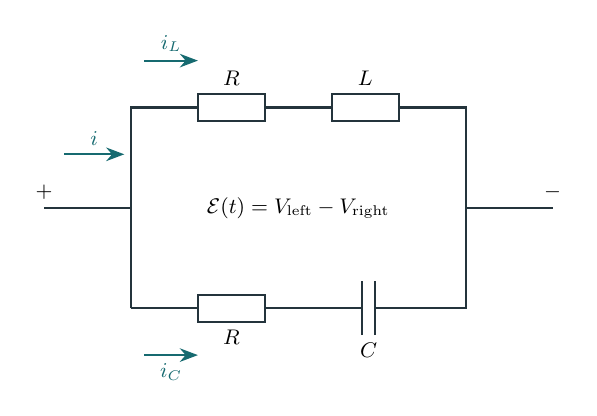
\begin{tikzpicture}[scale=.85,transform shape]

\draw[object] (0,0)--(0,3)--(1,3);
\draw[object] (1,2.8) rectangle (2,3.2);\node[above] at (1.5,3.2) {$R$};
\draw[object] (2,3)--(3,3);\draw[object] (3,2.8) rectangle (4,3.2);\node[above] at (3.5,3.2) {$L$};
\draw[object] (4,3)--(5,3)--(5,0)--(4,0);
\draw[object] (3.45,-.4)--(3.45,.4);\draw[object] (3.65,-.4)--(3.65,.4);
\draw[object] (4,0)--(3.65,0);\draw[object] (3.45,0)--(2,0);
\draw[object] (1,-.2) rectangle (2,.2);\node[below] at (1.5,-.2) {$R$};
\draw[object] (1,0)--(0,0);
\draw[object] (0,1.5)--(-1.3,1.5);\draw[object] (5,1.5)--(6.3,1.5);
\draw[motion] (-1,2.3)--(-.1,2.3) node[midway,above] {$i$};
\draw[motion] (.2,3.7)--(1,3.7) node[midway,above] {$i_L$};
\draw[motion] (.2,-.7)--(1,-.7) node[midway,below] {$i_C$};
\node[below] at (3.55,-.4) {$C$};
\node[above] at (-1.3,1.5) {$+$};\node[above] at (6.3,1.5) {$-$};
\node at (2.5,1.5) {$\mathcal E(t)=V_{\rm left}-V_{\rm right}$};

\end{tikzpicture}
\figcaption{图电试4.3\quad 两串联支路共用端电压，电流正方向均从左到右。}
\end{minipage}\end{center}

\Needspace{8\baselineskip}

\pdfbookmark[3]{题型定位}{q3-h0}

\subsection*{题型定位}

互补$RL,RC$支路的并联响应。三角恒等式先分开直流与二倍频，相量图用各支路电压直角三角形确定电流，再用投影说明无功分量抵消。复导纳把这一关系推广到任意频率，时域状态差则说明初始储能怎样进入总电流。

\Needspace{8\baselineskip}

\pdfbookmark[3]{知识点}{q3-h1}

\subsection*{知识点}

平方正弦包含直流和$2\omega$，两者分别求稳态。电感电压超前电流、电容电压滞后电流各$90^\circ$，串联支路电压相量相加。并联电流相量相加，导纳在复平面中相加。两个时间常数$L/R,RC$相同使导纳全频率恒为$1/R$。电感电流和电容电压是连续储能状态，其差的齐次响应决定额外端口电流。

\Needspace{8\baselineskip}

\pdfbookmark[3]{物理图像}{q3-h2}

\subsection*{物理图像}

题图两条支路共用电源，解图电试4.3D按电流为参考画出两个电压三角形，图A再把各电流旋到同一电压参考方向，正交分量上下抵消。图C把两支路和总电流画在相同时间轴上，端口过零时内部仍可有相反电流。图B标出$i_L$与$v_C/R$两个状态，它们的差值就是总电流中额外的指数项。

\Needspace{8\baselineskip}

\pdfbookmark[3]{解题入口}{q3-h3}

\subsection*{解题入口}

先展开$\sin^2\omega t$，在图旁写明实际交流角频率$\Omega=2\omega$，再计算$2R$与$R/2$两个电抗。用电压三角形求电流幅值和相位，随后分解同相、正交分量，最后放回负余弦输入。一般输入通分求$Y-1/R$，保留分子$R^2C-L$，由它同时说明条件的充分性与必要性。

\Needspace{8\baselineskip}

\pdfbookmark[3]{标准解法}{q3-h4}

\subsection*{标准解法}


图电试4.3中两支路共用同一端电压，总电流是支路电流的代数和。先展开电源：
\[
\mathcal E(t)=\frac{\mathcal E_0}{2}
-\frac{\mathcal E_0}{2}\cos2\omega t.
\]
输入分成直流和$2\omega$交流，后者的两支路电抗分别由$2\omega L$与$1/(2\omega C)$确定。

直流稳态时电感短接、电容开路，所以
\[
i_{L,{\rm dc}}=\frac{\mathcal E_0}{2R},\qquad
i_{C,{\rm dc}}=0.
\]
对交流分量记幅值$E_a=\mathcal E_0/2$、角频率$\Omega=2\omega$，则
\[
X_L=\Omega L=2R,\qquad X_C=\frac1{\Omega C}=\frac R2.
\]
\begin{center}\begin{minipage}{.98\linewidth}\centering
\begin{tikzpicture}[scale=.75,transform shape]

\node at (1.8,3.7) {支路电压三角形};
\draw[axis] (0,0)--(3.5,0) node[right] {$\widetilde E_a$};
\draw[motion] (0,0)--(.6,-1.2) node[midway,left] {$RI_{La}$};
\draw[force] (.6,-1.2)--(3,0) node[midway,below] {$2RI_{La}$};
\draw[motion] (0,0)--(2.4,1.2) node[midway,above left] {$RI_{Ca}$};
\draw[force] (2.4,1.2)--(3,0) node[midway,right] {$RI_{Ca}/2$};
\node at (1.8,-2.4) {$\phi_L+\phi_C=90^\circ$};
\begin{scope}[xshift=6cm]
\node at (1.8,3.7) {支路电流相加};
\draw[axis] (0,0)--(4.4,0) node[right] {同相};
\draw[axis] (0,-2.1)--(0,2.1);
\draw[motion] (0,0)--(.7,-1.4) node[below right] {$\widetilde I_{La}$};
\draw[motion] (0,0)--(2.8,1.4) node[above] {$\widetilde I_{Ca}$};
\draw[guide] (.7,-1.4)--(3.5,0)--(2.8,1.4);
\draw[force] (0,.08)--(3.5,.08) node[midway,above] {$\widetilde I_a=\widetilde E_a/R$};
\end{scope}

\end{tikzpicture}
\figcaption{解图电试4.3A\quad 先以交流电压为参考作图，再恢复输入负余弦的相位。}
\end{minipage}\end{center}
\begin{center}\begin{minipage}{.98\linewidth}\centering
\begin{tikzpicture}[scale=.8,transform shape]
\draw[axis] (0,0)--(2.8,0) node[right] {$I_L$};\draw[motion] (0,0)--(1,0) node[midway,below] {$I_LR$};\draw[motion] (1,0)--(1,2) node[midway,right] {$2I_LR$};\draw[force] (0,0)--(1,2) node[above] {$E_a$};\draw (0.5,0) arc(0:63.434949:.5);\node at (.8,.4) {$\phi_L$};\begin{scope}[xshift=6cm]\draw[axis] (0,0)--(3,0) node[right] {$I_C$};\draw[motion] (0,0)--(2,0) node[midway,above] {$I_CR$};\draw[motion] (2,0)--(2,-1) node[midway,right] {$I_CR/2$};\draw[force] (0,0)--(2,-1) node[right] {$E_a$};\draw (.6,0) arc(0:-26.565051:.6);\node at (1,-.5) {$\phi_C$};\end{scope}\node at (3,3) {两幅图各以支路电流为水平参考；电压横纵同尺度};
\end{tikzpicture}
\figcaption{解图电试4.3D\quad 两支路串联电压直角三角形决定电流相对端电压的相位}
\end{minipage}\end{center}
解图电试4.3D中两幅支路电压图各自以电流为参考：$RL$的水平电阻电压为$I_LR$，竖直向上电感电压为$2I_LR$；$RC$的水平电阻电压为$I_CR$，竖直向下电容电压为$I_CR/2$。电源电压都是同一条支路两电压的矢量和，故分别形成直角三角形。把每幅图旋到电源电压水平的共同参考后，再相加两电流。

解图电试4.3A以该交流电压相量$\widetilde E_a$为水平参考；$RL$支路的电阻电压与电流同相、电感电压超前电流$90^\circ$，两者直角相加。$RC$支路的电容电压落后电流$90^\circ$。据两个电压三角形，
\[
I_{La}=\frac{E_a}{\sqrt{R^2+(2R)^2}}
=\frac{E_a}{\sqrt5R},\qquad
I_{Ca}=\frac{E_a}{\sqrt{R^2+(R/2)^2}}
=\frac{2E_a}{\sqrt5R},
\]
\[
\tan\phi_L=2,\qquad \tan\phi_C=\frac12,\qquad
\phi_L+\phi_C=\frac\pi2.
\]
两支路电流相量互相垂直。电流的同相、正交分量分别为
\[
\begin{aligned}
I_{La}\cos\phi_L&=\frac{E_a}{5R},&
I_{La}\sin\phi_L&=\frac{2E_a}{5R},\\
I_{Ca}\cos\phi_C&=\frac{4E_a}{5R},&
I_{Ca}\sin\phi_C&=\frac{2E_a}{5R}.
\end{aligned}
\]
两电流与参考电压的夹角分别在下方$\phi_L$、上方$\phi_C$，所以第一支路的正交分量为负、第二支路为正；它们大小均为$2E_a/(5R)$。水平分量$E_a/(5R)+4E_a/(5R)=E_a/R$。也可由两电流互相垂直，以勾股关系得到合电流幅值$\sqrt{I_{La}^2+I_{Ca}^2}=E_a/R$，其方向由正交分量的相消确定。正交分量抵消，同相分量相加得$E_a/R$。代回输入交流项的负号，完整支路电流可写为
\[
\begin{aligned}
i_L(t)&=\frac{\mathcal E_0}{2R}
-\frac{\mathcal E_0}{10R}\cos2\omega t
-\frac{\mathcal E_0}{5R}\sin2\omega t,\\
i_C(t)&=-\frac{2\mathcal E_0}{5R}\cos2\omega t
+\frac{\mathcal E_0}{5R}\sin2\omega t.
\end{aligned}
\]
因此
\[
\boxed{i(t)=\frac{\mathcal E_0}{2R}(1-\cos2\omega t)
=\frac{\mathcal E_0}{R}\sin^2\omega t}.
\]
电容支路电流可以为负，总电流却始终非负。相量图只处理单一频率的交流分量，直流须另外叠加。

\begin{center}\begin{minipage}{.98\linewidth}\centering
\begin{tikzpicture}[scale=.8,transform shape]
\draw[axis] (0,0)--(10.7,0) node[right] {$\omega t$};
\draw[axis] (0,0)--(0,3.2) node[above] {$iR/\mathcal E_0$};\foreach \y/\lab in {0/-0.5,1.8/0.5,2.7/1}{\draw[thin] (0,\y)--(-.08,\y) node[left] {$\lab$};}
\node[above] at (5,3.5) {实线RL、虚线RC、细线端口；水平点线为零电流};
\draw[traj] plot coordinates {(0.000000000,1.620000000) (0.062500000,1.592309605) (0.125000000,1.565899691) (0.187500000,1.540933083) (0.250000000,1.517563709) (0.312500000,1.495935648) (0.375000000,1.476182246) (0.437500000,1.458425287) (0.500000000,1.442774250) (0.562500000,1.429325629) (0.625000000,1.418162338) (0.687500000,1.409353204) (0.750000000,1.402952537) (0.812500000,1.398999799) (0.875000000,1.397519361) (0.937500000,1.398520350) (1.000000000,1.401996595) (1.062500000,1.407926663) (1.125000000,1.416273994) (1.187500000,1.426987123) (1.250000000,1.440000000) (1.312500000,1.455232397) (1.375000000,1.472590401) (1.437500000,1.491966994) (1.500000000,1.513242713) (1.562500000,1.536286386) (1.625000000,1.560955941) (1.687500000,1.587099282) (1.750000000,1.614555227) (1.812500000,1.643154501) (1.875000000,1.672720779) (1.937500000,1.703071776) (2.000000000,1.734020368) (2.062500000,1.765375746) (2.125000000,1.796944594) (2.187500000,1.828532280) (2.250000000,1.859944055) (2.312500000,1.890986255) (2.375000000,1.921467494) (2.437500000,1.951199846) (2.500000000,1.980000000) (2.562500000,2.007690395) (2.625000000,2.034100309) (2.687500000,2.059066917) (2.750000000,2.082436291) (2.812500000,2.104064352) (2.875000000,2.123817754) (2.937500000,2.141574713) (3.000000000,2.157225750) (3.062500000,2.170674371) (3.125000000,2.181837662) (3.187500000,2.190646796) (3.250000000,2.197047463) (3.312500000,2.201000201) (3.375000000,2.202480639) (3.437500000,2.201479650) (3.500000000,2.198003405) (3.562500000,2.192073337) (3.625000000,2.183726006) (3.687500000,2.173012877) (3.750000000,2.160000000) (3.812500000,2.144767603) (3.875000000,2.127409599) (3.937500000,2.108033006) (4.000000000,2.086757287) (4.062500000,2.063713614) (4.125000000,2.039044059) (4.187500000,2.012900718) (4.250000000,1.985444773) (4.312500000,1.956845499) (4.375000000,1.927279221) (4.437500000,1.896928224) (4.500000000,1.865979632) (4.562500000,1.834624254) (4.625000000,1.803055406) (4.687500000,1.771467720) (4.750000000,1.740055945) (4.812500000,1.709013745) (4.875000000,1.678532506) (4.937500000,1.648800154) (5.000000000,1.620000000) (5.062500000,1.592309605) (5.125000000,1.565899691) (5.187500000,1.540933083) (5.250000000,1.517563709) (5.312500000,1.495935648) (5.375000000,1.476182246) (5.437500000,1.458425287) (5.500000000,1.442774250) (5.562500000,1.429325629) (5.625000000,1.418162338) (5.687500000,1.409353204) (5.750000000,1.402952537) (5.812500000,1.398999799) (5.875000000,1.397519361) (5.937500000,1.398520350) (6.000000000,1.401996595) (6.062500000,1.407926663) (6.125000000,1.416273994) (6.187500000,1.426987123) (6.250000000,1.440000000) (6.312500000,1.455232397) (6.375000000,1.472590401) (6.437500000,1.491966994) (6.500000000,1.513242713) (6.562500000,1.536286386) (6.625000000,1.560955941) (6.687500000,1.587099282) (6.750000000,1.614555227) (6.812500000,1.643154501) (6.875000000,1.672720779) (6.937500000,1.703071776) (7.000000000,1.734020368) (7.062500000,1.765375746) (7.125000000,1.796944594) (7.187500000,1.828532280) (7.250000000,1.859944055) (7.312500000,1.890986255) (7.375000000,1.921467494) (7.437500000,1.951199846) (7.500000000,1.980000000) (7.562500000,2.007690395) (7.625000000,2.034100309) (7.687500000,2.059066917) (7.750000000,2.082436291) (7.812500000,2.104064352) (7.875000000,2.123817754) (7.937500000,2.141574713) (8.000000000,2.157225750) (8.062500000,2.170674371) (8.125000000,2.181837662) (8.187500000,2.190646796) (8.250000000,2.197047463) (8.312500000,2.201000201) (8.375000000,2.202480639) (8.437500000,2.201479650) (8.500000000,2.198003405) (8.562500000,2.192073337) (8.625000000,2.183726006) (8.687500000,2.173012877) (8.750000000,2.160000000) (8.812500000,2.144767603) (8.875000000,2.127409599) (8.937500000,2.108033006) (9.000000000,2.086757287) (9.062500000,2.063713614) (9.125000000,2.039044059) (9.187500000,2.012900718) (9.250000000,1.985444773) (9.312500000,1.956845499) (9.375000000,1.927279221) (9.437500000,1.896928224) (9.500000000,1.865979632) (9.562500000,1.834624254) (9.625000000,1.803055406) (9.687500000,1.771467720) (9.750000000,1.740055945) (9.812500000,1.709013745) (9.875000000,1.678532506) (9.937500000,1.648800154) (10.000000000,1.620000000)};
\draw[dashed,thick,color=warm] plot coordinates {(0.000000000,0.180000000) (0.062500000,0.210464794) (0.125000000,0.245180802) (0.187500000,0.283933988) (0.250000000,0.326485426) (0.312500000,0.372572772) (0.375000000,0.421911882) (0.437500000,0.474198565) (0.500000000,0.529110455) (0.562500000,0.586309002) (0.625000000,0.645441559) (0.687500000,0.706143553) (0.750000000,0.768040736) (0.812500000,0.830751493) (0.875000000,0.893889189) (0.937500000,0.957064560) (1.000000000,1.019888110) (1.062500000,1.081972509) (1.125000000,1.142934988) (1.187500000,1.202399691) (1.250000000,1.260000000) (1.312500000,1.315380789) (1.375000000,1.368200617) (1.437500000,1.418133833) (1.500000000,1.464872582) (1.562500000,1.508128703) (1.625000000,1.547635509) (1.687500000,1.583149426) (1.750000000,1.614451500) (1.812500000,1.641348742) (1.875000000,1.663675324) (1.937500000,1.681293593) (2.000000000,1.694094927) (2.062500000,1.702000402) (2.125000000,1.704961277) (2.187500000,1.702959299) (2.250000000,1.696006810) (2.312500000,1.684146674) (2.375000000,1.667452013) (2.437500000,1.646025755) (2.500000000,1.620000000) (2.562500000,1.589535206) (2.625000000,1.554819198) (2.687500000,1.516066012) (2.750000000,1.473514574) (2.812500000,1.427427228) (2.875000000,1.378088118) (2.937500000,1.325801435) (3.000000000,1.270889545) (3.062500000,1.213690998) (3.125000000,1.154558441) (3.187500000,1.093856447) (3.250000000,1.031959264) (3.312500000,0.969248507) (3.375000000,0.906110811) (3.437500000,0.842935440) (3.500000000,0.780111890) (3.562500000,0.718027491) (3.625000000,0.657065012) (3.687500000,0.597600309) (3.750000000,0.540000000) (3.812500000,0.484619211) (3.875000000,0.431799383) (3.937500000,0.381866167) (4.000000000,0.335127418) (4.062500000,0.291871297) (4.125000000,0.252364491) (4.187500000,0.216850574) (4.250000000,0.185548500) (4.312500000,0.158651258) (4.375000000,0.136324676) (4.437500000,0.118706407) (4.500000000,0.105905073) (4.562500000,0.097999598) (4.625000000,0.095038723) (4.687500000,0.097040701) (4.750000000,0.103993190) (4.812500000,0.115853326) (4.875000000,0.132547987) (4.937500000,0.153974245) (5.000000000,0.180000000) (5.062500000,0.210464794) (5.125000000,0.245180802) (5.187500000,0.283933988) (5.250000000,0.326485426) (5.312500000,0.372572772) (5.375000000,0.421911882) (5.437500000,0.474198565) (5.500000000,0.529110455) (5.562500000,0.586309002) (5.625000000,0.645441559) (5.687500000,0.706143553) (5.750000000,0.768040736) (5.812500000,0.830751493) (5.875000000,0.893889189) (5.937500000,0.957064560) (6.000000000,1.019888110) (6.062500000,1.081972509) (6.125000000,1.142934988) (6.187500000,1.202399691) (6.250000000,1.260000000) (6.312500000,1.315380789) (6.375000000,1.368200617) (6.437500000,1.418133833) (6.500000000,1.464872582) (6.562500000,1.508128703) (6.625000000,1.547635509) (6.687500000,1.583149426) (6.750000000,1.614451500) (6.812500000,1.641348742) (6.875000000,1.663675324) (6.937500000,1.681293593) (7.000000000,1.694094927) (7.062500000,1.702000402) (7.125000000,1.704961277) (7.187500000,1.702959299) (7.250000000,1.696006810) (7.312500000,1.684146674) (7.375000000,1.667452013) (7.437500000,1.646025755) (7.500000000,1.620000000) (7.562500000,1.589535206) (7.625000000,1.554819198) (7.687500000,1.516066012) (7.750000000,1.473514574) (7.812500000,1.427427228) (7.875000000,1.378088118) (7.937500000,1.325801435) (8.000000000,1.270889545) (8.062500000,1.213690998) (8.125000000,1.154558441) (8.187500000,1.093856447) (8.250000000,1.031959264) (8.312500000,0.969248507) (8.375000000,0.906110811) (8.437500000,0.842935440) (8.500000000,0.780111890) (8.562500000,0.718027491) (8.625000000,0.657065012) (8.687500000,0.597600309) (8.750000000,0.540000000) (8.812500000,0.484619211) (8.875000000,0.431799383) (8.937500000,0.381866167) (9.000000000,0.335127418) (9.062500000,0.291871297) (9.125000000,0.252364491) (9.187500000,0.216850574) (9.250000000,0.185548500) (9.312500000,0.158651258) (9.375000000,0.136324676) (9.437500000,0.118706407) (9.500000000,0.105905073) (9.562500000,0.097999598) (9.625000000,0.095038723) (9.687500000,0.097040701) (9.750000000,0.103993190) (9.812500000,0.115853326) (9.875000000,0.132547987) (9.937500000,0.153974245) (10.000000000,0.180000000)};
\draw[thin,color=black] plot coordinates {(0.000000000,0.900000000) (0.062500000,0.902774400) (0.125000000,0.911080493) (0.187500000,0.924867072) (0.250000000,0.944049135) (0.312500000,0.968508421) (0.375000000,0.998094128) (0.437500000,1.032623852) (0.500000000,1.071884705) (0.562500000,1.115634631) (0.625000000,1.163603897) (0.687500000,1.215496757) (0.750000000,1.270993273) (0.812500000,1.329751292) (0.875000000,1.391408550) (0.937500000,1.455584911) (1.000000000,1.521884705) (1.062500000,1.589899173) (1.125000000,1.659208981) (1.187500000,1.729386814) (1.250000000,1.800000000) (1.312500000,1.870613186) (1.375000000,1.940791019) (1.437500000,2.010100827) (1.500000000,2.078115295) (1.562500000,2.144415089) (1.625000000,2.208591450) (1.687500000,2.270248708) (1.750000000,2.329006727) (1.812500000,2.384503243) (1.875000000,2.436396103) (1.937500000,2.484365369) (2.000000000,2.528115295) (2.062500000,2.567376148) (2.125000000,2.601905872) (2.187500000,2.631491579) (2.250000000,2.655950865) (2.312500000,2.675132928) (2.375000000,2.688919507) (2.437500000,2.697225600) (2.500000000,2.700000000) (2.562500000,2.697225600) (2.625000000,2.688919507) (2.687500000,2.675132928) (2.750000000,2.655950865) (2.812500000,2.631491579) (2.875000000,2.601905872) (2.937500000,2.567376148) (3.000000000,2.528115295) (3.062500000,2.484365369) (3.125000000,2.436396103) (3.187500000,2.384503243) (3.250000000,2.329006727) (3.312500000,2.270248708) (3.375000000,2.208591450) (3.437500000,2.144415089) (3.500000000,2.078115295) (3.562500000,2.010100827) (3.625000000,1.940791019) (3.687500000,1.870613186) (3.750000000,1.800000000) (3.812500000,1.729386814) (3.875000000,1.659208981) (3.937500000,1.589899173) (4.000000000,1.521884705) (4.062500000,1.455584911) (4.125000000,1.391408550) (4.187500000,1.329751292) (4.250000000,1.270993273) (4.312500000,1.215496757) (4.375000000,1.163603897) (4.437500000,1.115634631) (4.500000000,1.071884705) (4.562500000,1.032623852) (4.625000000,0.998094128) (4.687500000,0.968508421) (4.750000000,0.944049135) (4.812500000,0.924867072) (4.875000000,0.911080493) (4.937500000,0.902774400) (5.000000000,0.900000000) (5.062500000,0.902774400) (5.125000000,0.911080493) (5.187500000,0.924867072) (5.250000000,0.944049135) (5.312500000,0.968508421) (5.375000000,0.998094128) (5.437500000,1.032623852) (5.500000000,1.071884705) (5.562500000,1.115634631) (5.625000000,1.163603897) (5.687500000,1.215496757) (5.750000000,1.270993273) (5.812500000,1.329751292) (5.875000000,1.391408550) (5.937500000,1.455584911) (6.000000000,1.521884705) (6.062500000,1.589899173) (6.125000000,1.659208981) (6.187500000,1.729386814) (6.250000000,1.800000000) (6.312500000,1.870613186) (6.375000000,1.940791019) (6.437500000,2.010100827) (6.500000000,2.078115295) (6.562500000,2.144415089) (6.625000000,2.208591450) (6.687500000,2.270248708) (6.750000000,2.329006727) (6.812500000,2.384503243) (6.875000000,2.436396103) (6.937500000,2.484365369) (7.000000000,2.528115295) (7.062500000,2.567376148) (7.125000000,2.601905872) (7.187500000,2.631491579) (7.250000000,2.655950865) (7.312500000,2.675132928) (7.375000000,2.688919507) (7.437500000,2.697225600) (7.500000000,2.700000000) (7.562500000,2.697225600) (7.625000000,2.688919507) (7.687500000,2.675132928) (7.750000000,2.655950865) (7.812500000,2.631491579) (7.875000000,2.601905872) (7.937500000,2.567376148) (8.000000000,2.528115295) (8.062500000,2.484365369) (8.125000000,2.436396103) (8.187500000,2.384503243) (8.250000000,2.329006727) (8.312500000,2.270248708) (8.375000000,2.208591450) (8.437500000,2.144415089) (8.500000000,2.078115295) (8.562500000,2.010100827) (8.625000000,1.940791019) (8.687500000,1.870613186) (8.750000000,1.800000000) (8.812500000,1.729386814) (8.875000000,1.659208981) (8.937500000,1.589899173) (9.000000000,1.521884705) (9.062500000,1.455584911) (9.125000000,1.391408550) (9.187500000,1.329751292) (9.250000000,1.270993273) (9.312500000,1.215496757) (9.375000000,1.163603897) (9.437500000,1.115634631) (9.500000000,1.071884705) (9.562500000,1.032623852) (9.625000000,0.998094128) (9.687500000,0.968508421) (9.750000000,0.944049135) (9.812500000,0.924867072) (9.875000000,0.911080493) (9.937500000,0.902774400) (10.000000000,0.900000000)};
\node[below] at (0,-.12) {$0$};
\node[below] at (5,-.12) {$\pi$};
\node[below] at (10,-.12) {$2\pi$};
\draw[dotted] (0,.9)--(10,.9);\node[left] at (0,.9) {$0$};
\end{tikzpicture}
\figcaption{解图电试4.3C\quad 实线RL、虚线RC、细线端口；水平点线为零电流}
\end{minipage}\end{center}
解图电试4.3C在$t=0$给$i_L=2\mathcal E_0/(5R)$、$i_C=-2\mathcal E_0/(5R)$，两者相加为零。图中已经是周期稳态，电感、电容保存的瞬时状态使内部电流可在端口过零时继续存在。两支路的正弦正交项相反，余弦项与直流相加后形成非负的端口平方正弦。

第（2）问，任一非零角频率$\Omega$的输入电压相量记为$\widetilde E$。两支路导纳相加：
\[
Y(\Omega)=\frac1{R+\mathrm j\Omega L}
+\frac{\mathrm j\Omega C}{1+\mathrm j\Omega RC}.
\]
当
\[
\boxed{L=R^2C}
\]
时，时间常数满足$L/R=RC$。第一导纳的分母可写成$R(1+j\Omega RC)$，第二导纳已有同一因子，因此两个分母相同，故
\[
Y(\Omega)=\frac{1/R+\mathrm j\Omega C}
{1+\mathrm j\Omega RC}=\boxed{\frac1R}.
\]
通分时先把$1/R$写在同一分母下，分子中的常量和$\Omega^2LC$项逐项抵消，只剩与$R^2C-L$成正比的一阶虚数项。反过来，令$Y-1/R=0$，通分得
\[
Y-\frac1R=
\frac{\mathrm j\Omega(R^2C-L)}
{R(R+\mathrm j\Omega L)(1+\mathrm j\Omega RC)}.
\]
要在任一非零频率恒等于零，即得到同一匹配条件。直流导纳也为$1/R$，于是对
\[
\mathcal E(t)=E_{\rm dc}
+\sum_{n\ge1}E_n\cos(\Omega_nt+\psi_n)
\]
逐频率相加，稳态总电流恰为$\mathcal E(t)/R$。零初态时，相同的拉普拉斯导纳恒等式适用于一般分段连续输入，涵盖非周期驱动。
\begin{center}\begin{minipage}{.98\linewidth}\centering
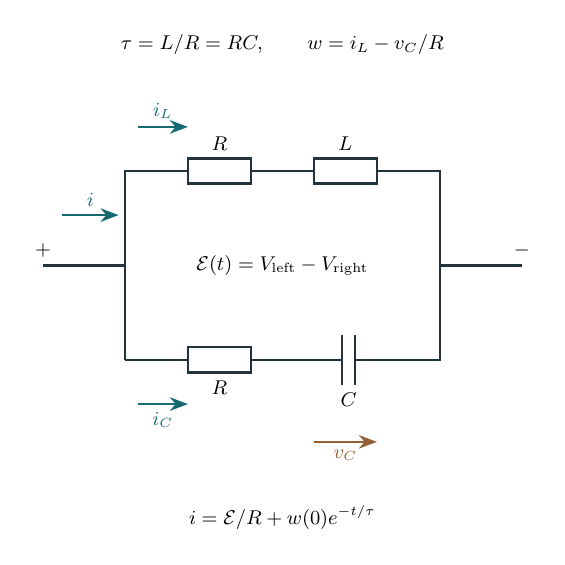
\begin{tikzpicture}[scale=.8,transform shape]

\draw[object] (0,0)--(0,3)--(1,3);
\draw[object] (1,2.8) rectangle (2,3.2);\node[above] at (1.5,3.2) {$R$};
\draw[object] (2,3)--(3,3);\draw[object] (3,2.8) rectangle (4,3.2);\node[above] at (3.5,3.2) {$L$};
\draw[object] (4,3)--(5,3)--(5,0)--(4,0);
\draw[object] (3.45,-.4)--(3.45,.4);\draw[object] (3.65,-.4)--(3.65,.4);
\draw[object] (4,0)--(3.65,0);\draw[object] (3.45,0)--(2,0);
\draw[object] (1,-.2) rectangle (2,.2);\node[below] at (1.5,-.2) {$R$};
\draw[object] (1,0)--(0,0);
\draw[object] (0,1.5)--(-1.3,1.5);\draw[object] (5,1.5)--(6.3,1.5);
\draw[motion] (-1,2.3)--(-.1,2.3) node[midway,above] {$i$};
\draw[motion] (.2,3.7)--(1,3.7) node[midway,above] {$i_L$};
\draw[motion] (.2,-.7)--(1,-.7) node[midway,below] {$i_C$};
\node[below] at (3.55,-.4) {$C$};
\node[above] at (-1.3,1.5) {$+$};\node[above] at (6.3,1.5) {$-$};
\node at (2.5,1.5) {$\mathcal E(t)=V_{\rm left}-V_{\rm right}$};

\draw[force] (3,-1.3)--(4,-1.3) node[midway,below] {$v_C$};
\node at (2.5,5) {$\tau=L/R=RC,\qquad w=i_L-v_C/R$};
\node at (2.5,-2.5) {$i=\mathcal E/R+w(0)e^{-t/\tau}$};

\end{tikzpicture}
\figcaption{解图电试4.3B\quad 保留初始电感电流和电容电压，端口额外响应由状态差决定。}
\end{minipage}\end{center}
第（3）问中，解图电试4.3B保留了电感、电容中的初始储能。支路方程为
\[
L\dot i_L+Ri_L=\mathcal E,\qquad
RC\dot v_C+v_C=\mathcal E,\qquad
i_C=\frac{\mathcal E-v_C}{R}.
\]
对电感方程除以$L$，对电容方程除以$R^2C$，匹配后两式的驱动项都是$\mathcal E/(R^2C)$，状态项系数都是$1/(RC)$。在$L=R^2C$下令$w=i_L-v_C/R$，相减可得
\[
\dot w=-\frac{w}{RC},\qquad
w(t)=\left[i_L(0)-\frac{v_C(0)}R\right]e^{-t/(RC)}.
\]
因此一般端口响应为
\[
\boxed{i(t)=\frac{\mathcal E(t)}R+
\left[i_L(0)-\frac{v_C(0)}R\right]e^{-t/(RC)}}.
\]
零状态、匹配初态$i_L(0)=v_C(0)/R$，以及暂态衰减后的稳态，都给端口纯电阻关系。即使初始能量非零，只要$w(0)=0$，这一自然响应也可在端口完全抵消；内部电流、电压及耗散仍实际存在。
这里总电流的恒等分解是$i=i_L+(\mathcal E-v_C)/R=\mathcal E/R+w$。状态差的一阶齐次方程中驱动完全相消，积分得到指数项，说明它的系数只由两个初值确定。电容电压取沿支路电流方向的电势降，所以它在$w$中带负号；电感电流取电源流入支路的方向，在$w$中带正号。匹配的内部状态仍有储能，并通过两电阻逐渐耗散。



\Needspace{8\baselineskip}

\pdfbookmark[3]{关键洞察}{q3-h5}

\subsection*{关键洞察}

两支路相等的是时间常数，单个支路电流仍有相位差。互补导纳使端口同相关系逐频率成立，内部储能状态仍按各自方程演化。匹配的非零初态$i_L(0)=v_C(0)/R$能在端口相消而在内部衰减，端口传递关系与内部能量变化可同时成立。失配初态的差值则给可测的指数电流。

\Needspace{8\baselineskip}

\pdfbookmark[3]{易错点}{q3-h6}

\subsection*{易错点}

用交流分量的频率$2\omega$计算电抗，直流部分另行叠加。相量图的参考电压可以先取正余弦，回到实际输入时保留负号。严格的$Y=1/R$同时限定导纳实部和虚部，单频虚部为零是较弱条件。一般初态在总电流中留下状态差的指数项，匹配初态则把这一项抵消。

\Needspace{8\baselineskip}

\pdfbookmark[3]{课堂讲解建议}{q3-h7}

\subsection*{课堂讲解建议}

让学生先在图D写电阻与电抗的长度比例，再把两幅图中的电流旋到共同电压方向，按图A计算投影。给出$t=0$的稳态支路电流，要求说明电源电动势为零时两支路为何仍各有电流。

完成复导纳通分后，把条件$L/R=RC$写成时间常数相等，再直接相减两条状态方程。给定$i_L(0)=I_0,v_C(0)=RI_0$且输入置零，让学生同时写端口电流、两电阻热功率和储能衰减。再把电容初始电压改为另一值，读出端口指数项的幅度，将稳态端口响应和初态指数响应放回同一组支路方程。

\Needspace{8\baselineskip}

\pdfbookmark[3]{变式训练}{q3-h8}

\subsection*{变式训练}

\begin{enumerate}
\Needspace{20\baselineskip}
\item 满足$L=R^2C$，从零状态接入恒压$E$，求两支路和端口电流。
\textbf{解：}变图电试4.3V1令$\tau=RC=L/R$。电感方程$\tau\dot i_L+i_L=E/R$给$i_L=(E/R)(1-e^{-t/\tau})$，电容电压为$v_C=E(1-e^{-t/\tau})$，所以$i_C=(E-v_C)/R=(E/R)e^{-t/\tau}$。两支路一增一减，端口从接通后即为$E/R$。接通瞬间电感电流仍为零，电容支路承担全部电流；长期则由电感支路承担。
\begin{center}\begin{minipage}{.98\linewidth}\centering
\begin{tikzpicture}[scale=.8,transform shape]
\draw[axis] (0,0)--(10.7,0) node[right] {$t/\tau$};
\draw[axis] (0,0)--(0,3.2) node[above] {$iR/E$};\foreach \y/\lab in {0/0,1.4/0.5,2.8/1}{\draw[thin] (0,\y)--(-.08,\y) node[left] {$\lab$};}
\node[above] at (5,3.5) {RL电流上升，RC电流下降，总和恒为1};
\draw[traj] plot coordinates {(0.000000000,0.000000000) (0.083333333,0.114269520) (0.166666667,0.223875639) (0.250000000,0.329008673) (0.333333333,0.429851170) (0.416666667,0.526578231) (0.500000000,0.619357807) (0.583333333,0.708350999) (0.666666667,0.793712330) (0.750000000,0.875590019) (0.833333333,0.954126235) (0.916666667,1.029457346) (1.000000000,1.101714153) (1.083333333,1.171022120) (1.166666667,1.237501592) (1.250000000,1.301268000) (1.333333333,1.362432067) (1.416666667,1.421099995) (1.500000000,1.477373652) (1.583333333,1.531350752) (1.666666667,1.583125016) (1.750000000,1.632786345) (1.833333333,1.680420968) (1.916666667,1.726111596) (2.000000000,1.769937565) (2.083333333,1.811974972) (2.166666667,1.852296810) (2.250000000,1.890973091) (2.333333333,1.928070973) (2.416666667,1.963654870) (2.500000000,1.997786569) (2.583333333,2.030525334) (2.666666667,2.061928013) (2.750000000,2.092049132) (2.833333333,2.120940991) (2.916666667,2.148653758) (3.000000000,2.175235552) (3.083333333,2.200732528) (3.166666667,2.225188959) (3.250000000,2.248647309) (3.333333333,2.271148312) (3.416666667,2.292731037) (3.500000000,2.313432958) (3.583333333,2.333290023) (3.666666667,2.352336711) (3.750000000,2.370606093) (3.833333333,2.388129891) (3.916666667,2.404938534) (4.000000000,2.421061207) (4.083333333,2.436525905) (4.166666667,2.451359480) (4.250000000,2.465587689) (4.333333333,2.479235237) (4.416666667,2.492325821) (4.500000000,2.504882171) (4.583333333,2.516926090) (4.666666667,2.528478490) (4.750000000,2.539559430) (4.833333333,2.550188151) (4.916666667,2.560383108) (5.000000000,2.570162004) (5.083333333,2.579541817) (5.166666667,2.588538835) (5.250000000,2.597168680) (5.333333333,2.605446337) (5.416666667,2.613386177) (5.500000000,2.621001989) (5.583333333,2.628306995) (5.666666667,2.635313879) (5.750000000,2.642034809) (5.833333333,2.648481455) (5.916666667,2.654665009) (6.000000000,2.660596209) (6.083333333,2.666285353) (6.166666667,2.671742320) (6.250000000,2.676976586) (6.333333333,2.681997238) (6.416666667,2.686812995) (6.500000000,2.691432218) (6.583333333,2.695862928) (6.666666667,2.700112819) (6.750000000,2.704189269) (6.833333333,2.708099357) (6.916666667,2.711849872) (7.000000000,2.715447326) (7.083333333,2.718897967) (7.166666667,2.722207785) (7.250000000,2.725382527) (7.333333333,2.728427707) (7.416666667,2.731348611) (7.500000000,2.734150312) (7.583333333,2.736837673) (7.666666667,2.739415362) (7.750000000,2.741887854) (7.833333333,2.744259442) (7.916666667,2.746534245) (8.000000000,2.748716211) (8.083333333,2.750809130) (8.166666667,2.752816636) (8.250000000,2.754742215) (8.333333333,2.756589210) (8.416666667,2.758360828) (8.500000000,2.760060145) (8.583333333,2.761690112) (8.666666667,2.763253560) (8.750000000,2.764753202) (8.833333333,2.766191643) (8.916666667,2.767571380) (9.000000000,2.768894810) (9.083333333,2.770164229) (9.166666667,2.771381843) (9.250000000,2.772549766) (9.333333333,2.773670025) (9.416666667,2.774744565) (9.500000000,2.775775253) (9.583333333,2.776763878) (9.666666667,2.777712157) (9.750000000,2.778621736) (9.833333333,2.779494195) (9.916666667,2.780331048) (10.000000000,2.781133748)};
\draw[dashed,thick,color=warm] plot coordinates {(0.000000000,2.800000000) (0.083333333,2.685730480) (0.166666667,2.576124361) (0.250000000,2.470991327) (0.333333333,2.370148830) (0.416666667,2.273421769) (0.500000000,2.180642193) (0.583333333,2.091649001) (0.666666667,2.006287670) (0.750000000,1.924409981) (0.833333333,1.845873765) (0.916666667,1.770542654) (1.000000000,1.698285847) (1.083333333,1.628977880) (1.166666667,1.562498408) (1.250000000,1.498732000) (1.333333333,1.437567933) (1.416666667,1.378900005) (1.500000000,1.322626348) (1.583333333,1.268649248) (1.666666667,1.216874984) (1.750000000,1.167213655) (1.833333333,1.119579032) (1.916666667,1.073888404) (2.000000000,1.030062435) (2.083333333,0.988025028) (2.166666667,0.947703190) (2.250000000,0.909026909) (2.333333333,0.871929027) (2.416666667,0.836345130) (2.500000000,0.802213431) (2.583333333,0.769474666) (2.666666667,0.738071987) (2.750000000,0.707950868) (2.833333333,0.679059009) (2.916666667,0.651346242) (3.000000000,0.624764448) (3.083333333,0.599267472) (3.166666667,0.574811041) (3.250000000,0.551352691) (3.333333333,0.528851688) (3.416666667,0.507268963) (3.500000000,0.486567042) (3.583333333,0.466709977) (3.666666667,0.447663289) (3.750000000,0.429393907) (3.833333333,0.411870109) (3.916666667,0.395061466) (4.000000000,0.378938793) (4.083333333,0.363474095) (4.166666667,0.348640520) (4.250000000,0.334412311) (4.333333333,0.320764763) (4.416666667,0.307674179) (4.500000000,0.295117829) (4.583333333,0.283073910) (4.666666667,0.271521510) (4.750000000,0.260440570) (4.833333333,0.249811849) (4.916666667,0.239616892) (5.000000000,0.229837996) (5.083333333,0.220458183) (5.166666667,0.211461165) (5.250000000,0.202831320) (5.333333333,0.194553663) (5.416666667,0.186613823) (5.500000000,0.178998011) (5.583333333,0.171693005) (5.666666667,0.164686121) (5.750000000,0.157965191) (5.833333333,0.151518545) (5.916666667,0.145334991) (6.000000000,0.139403791) (6.083333333,0.133714647) (6.166666667,0.128257680) (6.250000000,0.123023414) (6.333333333,0.118002762) (6.416666667,0.113187005) (6.500000000,0.108567782) (6.583333333,0.104137072) (6.666666667,0.099887181) (6.750000000,0.095810731) (6.833333333,0.091900643) (6.916666667,0.088150128) (7.000000000,0.084552674) (7.083333333,0.081102033) (7.166666667,0.077792215) (7.250000000,0.074617473) (7.333333333,0.071572293) (7.416666667,0.068651389) (7.500000000,0.065849688) (7.583333333,0.063162327) (7.666666667,0.060584638) (7.750000000,0.058112146) (7.833333333,0.055740558) (7.916666667,0.053465755) (8.000000000,0.051283789) (8.083333333,0.049190870) (8.166666667,0.047183364) (8.250000000,0.045257785) (8.333333333,0.043410790) (8.416666667,0.041639172) (8.500000000,0.039939855) (8.583333333,0.038309888) (8.666666667,0.036746440) (8.750000000,0.035246798) (8.833333333,0.033808357) (8.916666667,0.032428620) (9.000000000,0.031105190) (9.083333333,0.029835771) (9.166666667,0.028618157) (9.250000000,0.027450234) (9.333333333,0.026329975) (9.416666667,0.025255435) (9.500000000,0.024224747) (9.583333333,0.023236122) (9.666666667,0.022287843) (9.750000000,0.021378264) (9.833333333,0.020505805) (9.916666667,0.019668952) (10.000000000,0.018866252)};
\node[below] at (0,-.12) {$0$};
\node[below] at (5,-.12) {$2.5$};
\node[below] at (10,-.12) {$5$};
\end{tikzpicture}
\figcaption{变图电试4.3V1\quad RL电流上升，RC电流下降，总和恒为1}
\end{minipage}\end{center}

\Needspace{20\baselineskip}
\item 输入电压置零，初态$i_L(0)=I_0,v_C(0)=RI_0$，求端口电流和总耗散能量。
\textbf{解：}变图电试4.3V2两支路初值相匹配，分别给$i_L=I_0e^{-t/\tau}$、$v_C=RI_0e^{-t/\tau}$、$i_C=-I_0e^{-t/\tau}$，所以端口电流为零。两电阻的功率之和为$2RI_0^2e^{-2t/\tau}$，时间积分为$R\tau I_0^2=LI_0^2$。初始储能为$LI_0^2/2+C(RI_0)^2/2=LI_0^2$，恰全部转为热。零电压条件可由理想电压源置零后的短路实现，内部电流在两支路之间回流。
\begin{center}\begin{minipage}{.98\linewidth}\centering
\begin{tikzpicture}[scale=.8,transform shape]
\draw[axis] (0,0)--(10.7,0) node[right] {$t/\tau$};
\draw[axis] (0,0)--(0,3.2) node[above] {$i/I_0$};\foreach \y/\lab in {0.13/-1,2.73/1}{\draw[thin] (0,\y)--(-.08,\y) node[left] {$\lab$};}
\node[above] at (5,3.5) {两支路相反电流抵消端口响应，内部储能衰减};
\draw[traj] plot coordinates {(0.000000000,2.730000000) (0.083333333,2.676946294) (0.166666667,2.626057739) (0.250000000,2.577245973) (0.333333333,2.530426242) (0.416666667,2.485517250) (0.500000000,2.442441018) (0.583333333,2.401122750) (0.666666667,2.361490704) (0.750000000,2.323476062) (0.833333333,2.287012819) (0.916666667,2.252037661) (1.000000000,2.218489858) (1.083333333,2.186311158) (1.166666667,2.155445690) (1.250000000,2.125839857) (1.333333333,2.097442255) (1.416666667,2.070203574) (1.500000000,2.044076519) (1.583333333,2.019015722) (1.666666667,1.994977671) (1.750000000,1.971920626) (1.833333333,1.949804551) (1.916666667,1.928591045) (2.000000000,1.908243274) (2.083333333,1.888725906) (2.166666667,1.870005053) (2.250000000,1.852048208) (2.333333333,1.834824191) (2.416666667,1.818303096) (2.500000000,1.802456236) (2.583333333,1.787256095) (2.666666667,1.772676280) (2.750000000,1.758691475) (2.833333333,1.745277397) (2.916666667,1.732410755) (3.000000000,1.720069208) (3.083333333,1.708231326) (3.166666667,1.696876555) (3.250000000,1.685985178) (3.333333333,1.675538284) (3.416666667,1.665517733) (3.500000000,1.655906126) (3.583333333,1.646686775) (3.666666667,1.637843670) (3.750000000,1.629361457) (3.833333333,1.621225408) (3.916666667,1.613421395) (4.000000000,1.605935868) (4.083333333,1.598755830) (4.166666667,1.591868813) (4.250000000,1.585262859) (4.333333333,1.578926497) (4.416666667,1.572848726) (4.500000000,1.567018992) (4.583333333,1.561427172) (4.666666667,1.556063558) (4.750000000,1.550918836) (4.833333333,1.545984073) (4.916666667,1.541250700) (5.000000000,1.536710498) (5.083333333,1.532355585) (5.166666667,1.528178398) (5.250000000,1.524171684) (5.333333333,1.520328487) (5.416666667,1.516642132) (5.500000000,1.513106220) (5.583333333,1.509714610) (5.666666667,1.506461413) (5.750000000,1.503340981) (5.833333333,1.500347896) (5.916666667,1.497476960) (6.000000000,1.494723189) (6.083333333,1.492081800) (6.166666667,1.489548208) (6.250000000,1.487118014) (6.333333333,1.484786997) (6.416666667,1.482551109) (6.500000000,1.480406470) (6.583333333,1.478349355) (6.666666667,1.476376191) (6.750000000,1.474483554) (6.833333333,1.472668156) (6.916666667,1.470926845) (7.000000000,1.469256598) (7.083333333,1.467654515) (7.166666667,1.466117814) (7.250000000,1.464643827) (7.333333333,1.463229993) (7.416666667,1.461873859) (7.500000000,1.460573070) (7.583333333,1.459325366) (7.666666667,1.458128582) (7.750000000,1.456980639) (7.833333333,1.455879545) (7.916666667,1.454823386) (8.000000000,1.453810331) (8.083333333,1.452838618) (8.166666667,1.451906562) (8.250000000,1.451012543) (8.333333333,1.450155010) (8.416666667,1.449332473) (8.500000000,1.448543504) (8.583333333,1.447786734) (8.666666667,1.447060847) (8.750000000,1.446364585) (8.833333333,1.445696737) (8.916666667,1.445056145) (9.000000000,1.444441695) (9.083333333,1.443852322) (9.166666667,1.443287001) (9.250000000,1.442744752) (9.333333333,1.442224631) (9.416666667,1.441725737) (9.500000000,1.441247204) (9.583333333,1.440788199) (9.666666667,1.440347927) (9.750000000,1.439925622) (9.833333333,1.439520552) (9.916666667,1.439132014) (10.000000000,1.438759331)};
\draw[dashed,thick,color=warm] plot coordinates {(0.000000000,0.130000000) (0.083333333,0.183053706) (0.166666667,0.233942261) (0.250000000,0.282754027) (0.333333333,0.329573758) (0.416666667,0.374482750) (0.500000000,0.417558982) (0.583333333,0.458877250) (0.666666667,0.498509296) (0.750000000,0.536523938) (0.833333333,0.572987181) (0.916666667,0.607962339) (1.000000000,0.641510142) (1.083333333,0.673688842) (1.166666667,0.704554310) (1.250000000,0.734160143) (1.333333333,0.762557745) (1.416666667,0.789796426) (1.500000000,0.815923481) (1.583333333,0.840984278) (1.666666667,0.865022329) (1.750000000,0.888079374) (1.833333333,0.910195449) (1.916666667,0.931408955) (2.000000000,0.951756726) (2.083333333,0.971274094) (2.166666667,0.989994947) (2.250000000,1.007951792) (2.333333333,1.025175809) (2.416666667,1.041696904) (2.500000000,1.057543764) (2.583333333,1.072743905) (2.666666667,1.087323720) (2.750000000,1.101308525) (2.833333333,1.114722603) (2.916666667,1.127589245) (3.000000000,1.139930792) (3.083333333,1.151768674) (3.166666667,1.163123445) (3.250000000,1.174014822) (3.333333333,1.184461716) (3.416666667,1.194482267) (3.500000000,1.204093874) (3.583333333,1.213313225) (3.666666667,1.222156330) (3.750000000,1.230638543) (3.833333333,1.238774592) (3.916666667,1.246578605) (4.000000000,1.254064132) (4.083333333,1.261244170) (4.166666667,1.268131187) (4.250000000,1.274737141) (4.333333333,1.281073503) (4.416666667,1.287151274) (4.500000000,1.292981008) (4.583333333,1.298572828) (4.666666667,1.303936442) (4.750000000,1.309081164) (4.833333333,1.314015927) (4.916666667,1.318749300) (5.000000000,1.323289502) (5.083333333,1.327644415) (5.166666667,1.331821602) (5.250000000,1.335828316) (5.333333333,1.339671513) (5.416666667,1.343357868) (5.500000000,1.346893780) (5.583333333,1.350285390) (5.666666667,1.353538587) (5.750000000,1.356659019) (5.833333333,1.359652104) (5.916666667,1.362523040) (6.000000000,1.365276811) (6.083333333,1.367918200) (6.166666667,1.370451792) (6.250000000,1.372881986) (6.333333333,1.375213003) (6.416666667,1.377448891) (6.500000000,1.379593530) (6.583333333,1.381650645) (6.666666667,1.383623809) (6.750000000,1.385516446) (6.833333333,1.387331844) (6.916666667,1.389073155) (7.000000000,1.390743402) (7.083333333,1.392345485) (7.166666667,1.393882186) (7.250000000,1.395356173) (7.333333333,1.396770007) (7.416666667,1.398126141) (7.500000000,1.399426930) (7.583333333,1.400674634) (7.666666667,1.401871418) (7.750000000,1.403019361) (7.833333333,1.404120455) (7.916666667,1.405176614) (8.000000000,1.406189669) (8.083333333,1.407161382) (8.166666667,1.408093438) (8.250000000,1.408987457) (8.333333333,1.409844990) (8.416666667,1.410667527) (8.500000000,1.411456496) (8.583333333,1.412213266) (8.666666667,1.412939153) (8.750000000,1.413635415) (8.833333333,1.414303263) (8.916666667,1.414943855) (9.000000000,1.415558305) (9.083333333,1.416147678) (9.166666667,1.416712999) (9.250000000,1.417255248) (9.333333333,1.417775369) (9.416666667,1.418274263) (9.500000000,1.418752796) (9.583333333,1.419211801) (9.666666667,1.419652073) (9.750000000,1.420074378) (9.833333333,1.420479448) (9.916666667,1.420867986) (10.000000000,1.421240669)};
\node[below] at (0,-.12) {$0$};
\node[below] at (5,-.12) {$2.5$};
\node[below] at (10,-.12) {$5$};
\draw[dotted] (0,1.43)--(10,1.43);\node[left] at (0,1.43) {$0$};
\end{tikzpicture}
\figcaption{变图电试4.3V2\quad 两支路相反电流抵消端口响应，内部储能衰减}
\end{minipage}\end{center}

\Needspace{20\baselineskip}
\item 只在一个非零频率要求总导纳严格等于$1/R$，是否仍需匹配？若只要求端口同相，又有何结果？
\textbf{解：}变图电试4.3V3由主解的$Y-1/R$因式，非零频率严格相等给$L=R^2C$。若只要求虚部为零，记$\kappa=L/(R^2C)$、$\nu=\Omega RC$，则$R\Im Y=\nu(\kappa-1)(\kappa\nu^2-1)/[(1+\kappa^2\nu^2)(1+\nu^2)]$。失配时也在$\nu=1/\sqrt\kappa$即$\Omega=1/\sqrt{LC}$同相，但此时$Y=2/[R(1+\kappa)]$，一般不同于$1/R$。图中的过零点只说明相位关系，导纳实部还由同一式确定。
\begin{center}\begin{minipage}{.98\linewidth}\centering
\begin{tikzpicture}[scale=.8,transform shape]
\draw[axis] (0,0)--(10.7,0) node[right] {$\nu=\Omega RC$};
\draw[axis] (0,0)--(0,3.2) node[above] {$R\Im Y$};\foreach \y/\lab in {0.16/-0.1,1.76/0.1,2.56/0.2}{\draw[thin] (0,\y)--(-.08,\y) node[left] {$\lab$};}
\node[above] at (5,3.5) {示例$\kappa=2$，非零过零点为$1/\sqrt2$};
\draw[traj] plot coordinates {(0.125000000,0.566923286) (0.207291667,0.327645042) (0.289583333,0.115465452) (0.371875000,-0.062243238) (0.454166667,-0.200799864) (0.536458333,-0.298223596) (0.618750000,-0.354945629) (0.701041667,-0.373331265) (0.783333333,-0.357124539) (0.865625000,-0.310906635) (0.947916667,-0.239627563) (1.030208333,-0.148239368) (1.112500000,-0.041435224) (1.194791667,0.076516304) (1.277083333,0.201859657) (1.359375000,0.331382813) (1.441666667,0.462407722) (1.523958333,0.592755331) (1.606250000,0.720696375) (1.688541667,0.844895952) (1.770833333,0.964357287) (1.853125000,1.078368067) (1.935416667,1.186451292) (2.017708333,1.288321544) (2.100000000,1.383846947) (2.182291667,1.473016643) (2.264583333,1.555913403) (2.346875000,1.632690831) (2.429166667,1.703554630) (2.511458333,1.768747354) (2.593750000,1.828536133) (2.676041667,1.883202905) (2.758333333,1.933036733) (2.840625000,1.978327840) (2.922916667,2.019363064) (3.005208333,2.056422455) (3.087500000,2.089776797) (3.169791667,2.119685881) (3.252083333,2.146397355) (3.334375000,2.170146047) (3.416666667,2.191153644) (3.498958333,2.209628649) (3.581250000,2.225766549) (3.663541667,2.239750135) (3.745833333,2.251749937) (3.828125000,2.261924733) (3.910416667,2.270422112) (3.992708333,2.277379064) (4.075000000,2.282922582) (4.157291667,2.287170264) (4.239583333,2.290230909) (4.321875000,2.292205093) (4.404166667,2.293185728) (4.486458333,2.293258593) (4.568750000,2.292502840) (4.651041667,2.290991476) (4.733333333,2.288791811) (4.815625000,2.285965880) (4.897916667,2.282570843) (4.980208333,2.278659353) (5.062500000,2.274279897) (5.144791667,2.269477119) (5.227083333,2.264292115) (5.309375000,2.258762707) (5.391666667,2.252923701) (5.473958333,2.246807116) (5.556250000,2.240442409) (5.638541667,2.233856668) (5.720833333,2.227074802) (5.803125000,2.220119712) (5.885416667,2.213012444) (5.967708333,2.205772340) (6.050000000,2.198417165) (6.132291667,2.190963239) (6.214583333,2.183425540) (6.296875000,2.175817817) (6.379166667,2.168152685) (6.461458333,2.160441708) (6.543750000,2.152695486) (6.626041667,2.144923731) (6.708333333,2.137135332) (6.790625000,2.129338422) (6.872916667,2.121540436) (6.955208333,2.113748165) (7.037500000,2.105967805) (7.119791667,2.098205007) (7.202083333,2.090464914) (7.284375000,2.082752205) (7.366666667,2.075071127) (7.448958333,2.067425533) (7.531250000,2.059818907) (7.613541667,2.052254399) (7.695833333,2.044734843) (7.778125000,2.037262791) (7.860416667,2.029840526) (7.942708333,2.022470090) (8.025000000,2.015153297) (8.107291667,2.007891756) (8.189583333,2.000686882) (8.271875000,1.993539916) (8.354166667,1.986451935) (8.436458333,1.979423867) (8.518750000,1.972456502) (8.601041667,1.965550504) (8.683333333,1.958706420) (8.765625000,1.951924690) (8.847916667,1.945205653) (8.930208333,1.938549562) (9.012500000,1.931956584) (9.094791667,1.925426809) (9.177083333,1.918960260) (9.259375000,1.912556893) (9.341666667,1.906216609) (9.423958333,1.899939252) (9.506250000,1.893724621) (9.588541667,1.887572466) (9.670833333,1.881482500) (9.753125000,1.875454399) (9.835416667,1.869487805) (9.917708333,1.863582329) (10.000000000,1.857737557)};
\node[below] at (0,-.12) {$0$极限};
\node[below] at (1.7677669529663687,-.12) {$1/\sqrt2$};
\node[below] at (10,-.12) {$4$};
\draw[dotted] (0,.96)--(10,.96);\node[left] at (0,.96) {$0$};
\end{tikzpicture}
\figcaption{变图电试4.3V3\quad 示例$\kappa=2$，非零过零点为$1/\sqrt2$}
\end{minipage}\end{center}

\Needspace{20\baselineskip}
\item 取$R=2\,\Omega,C=1\,\mathrm F,L=4\,\mathrm H$，初态$i_L(0)=3\,\mathrm A,v_C(0)=2\,\mathrm V$。求任意输入下的端口电流。
\textbf{解：}变图电试4.3V4时间常数为$\tau=2\,\mathrm s$，初始状态差$w_0=3-2/2=2\,\mathrm A$。因此$i(t)=\mathcal E(t)/(2\,\Omega)+(2\,\mathrm A)e^{-t/(2\,\mathrm s)}$。输入波形只决定第一项，失配初态决定第二项。若输入为零，端口从$2\,\mathrm A$指数衰减；在$t=2\,\mathrm s$降至$2/e\,\mathrm A$。若把电容初始电压改为$6\,\mathrm V$，状态差为零，额外端口电流随之消失。
\begin{center}\begin{minipage}{.98\linewidth}\centering
\begin{tikzpicture}[scale=.8,transform shape]
\draw[axis] (0,0)--(10.7,0) node[right] {$t/\mathrm s$};
\draw[axis] (0,0)--(0,3.2) node[above] {$\Delta i/\mathrm A$};\foreach \y/\lab in {0/0,1.4/1,2.8/2}{\draw[thin] (0,\y)--(-.08,\y) node[left] {$\lab$};}
\node[above] at (5,3.5) {初始状态差为2A，按时间常数2s衰减};
\draw[traj] plot coordinates {(0.000000000,2.800000000) (0.083333333,2.685730480) (0.166666667,2.576124361) (0.250000000,2.470991327) (0.333333333,2.370148830) (0.416666667,2.273421769) (0.500000000,2.180642193) (0.583333333,2.091649001) (0.666666667,2.006287670) (0.750000000,1.924409981) (0.833333333,1.845873765) (0.916666667,1.770542654) (1.000000000,1.698285847) (1.083333333,1.628977880) (1.166666667,1.562498408) (1.250000000,1.498732000) (1.333333333,1.437567933) (1.416666667,1.378900005) (1.500000000,1.322626348) (1.583333333,1.268649248) (1.666666667,1.216874984) (1.750000000,1.167213655) (1.833333333,1.119579032) (1.916666667,1.073888404) (2.000000000,1.030062435) (2.083333333,0.988025028) (2.166666667,0.947703190) (2.250000000,0.909026909) (2.333333333,0.871929027) (2.416666667,0.836345130) (2.500000000,0.802213431) (2.583333333,0.769474666) (2.666666667,0.738071987) (2.750000000,0.707950868) (2.833333333,0.679059009) (2.916666667,0.651346242) (3.000000000,0.624764448) (3.083333333,0.599267472) (3.166666667,0.574811041) (3.250000000,0.551352691) (3.333333333,0.528851688) (3.416666667,0.507268963) (3.500000000,0.486567042) (3.583333333,0.466709977) (3.666666667,0.447663289) (3.750000000,0.429393907) (3.833333333,0.411870109) (3.916666667,0.395061466) (4.000000000,0.378938793) (4.083333333,0.363474095) (4.166666667,0.348640520) (4.250000000,0.334412311) (4.333333333,0.320764763) (4.416666667,0.307674179) (4.500000000,0.295117829) (4.583333333,0.283073910) (4.666666667,0.271521510) (4.750000000,0.260440570) (4.833333333,0.249811849) (4.916666667,0.239616892) (5.000000000,0.229837996) (5.083333333,0.220458183) (5.166666667,0.211461165) (5.250000000,0.202831320) (5.333333333,0.194553663) (5.416666667,0.186613823) (5.500000000,0.178998011) (5.583333333,0.171693005) (5.666666667,0.164686121) (5.750000000,0.157965191) (5.833333333,0.151518545) (5.916666667,0.145334991) (6.000000000,0.139403791) (6.083333333,0.133714647) (6.166666667,0.128257680) (6.250000000,0.123023414) (6.333333333,0.118002762) (6.416666667,0.113187005) (6.500000000,0.108567782) (6.583333333,0.104137072) (6.666666667,0.099887181) (6.750000000,0.095810731) (6.833333333,0.091900643) (6.916666667,0.088150128) (7.000000000,0.084552674) (7.083333333,0.081102033) (7.166666667,0.077792215) (7.250000000,0.074617473) (7.333333333,0.071572293) (7.416666667,0.068651389) (7.500000000,0.065849688) (7.583333333,0.063162327) (7.666666667,0.060584638) (7.750000000,0.058112146) (7.833333333,0.055740558) (7.916666667,0.053465755) (8.000000000,0.051283789) (8.083333333,0.049190870) (8.166666667,0.047183364) (8.250000000,0.045257785) (8.333333333,0.043410790) (8.416666667,0.041639172) (8.500000000,0.039939855) (8.583333333,0.038309888) (8.666666667,0.036746440) (8.750000000,0.035246798) (8.833333333,0.033808357) (8.916666667,0.032428620) (9.000000000,0.031105190) (9.083333333,0.029835771) (9.166666667,0.028618157) (9.250000000,0.027450234) (9.333333333,0.026329975) (9.416666667,0.025255435) (9.500000000,0.024224747) (9.583333333,0.023236122) (9.666666667,0.022287843) (9.750000000,0.021378264) (9.833333333,0.020505805) (9.916666667,0.019668952) (10.000000000,0.018866252)};
\node[below] at (0,-.12) {$0$};
\node[below] at (5,-.12) {$5$};
\node[below] at (10,-.12) {$10$};
\end{tikzpicture}
\figcaption{变图电试4.3V4\quad 初始状态差为2A，按时间常数2s衰减}
\end{minipage}\end{center}

\Needspace{20\baselineskip}
\item 两串联支路的电阻分别为$R_a,R_b$，求端口在全部频率等效为同一个纯电阻的条件。
\textbf{解：}变图电试4.3V5的导纳为$Y=1/(R_a+j\Omega L)+j\Omega C/(1+j\Omega R_bC)$。低频极限为$1/R_a$，高频极限为$1/R_b$，频率无关要求$R_a=R_b=R$。代回后由$Y-1/R$的因式得到$L=R^2C$。这些条件同时成立便使整个导纳恒为$1/R$，既满足两个频率端的极限，又使中间全部频率的虚部相消。
\begin{center}\begin{minipage}{.98\linewidth}\centering
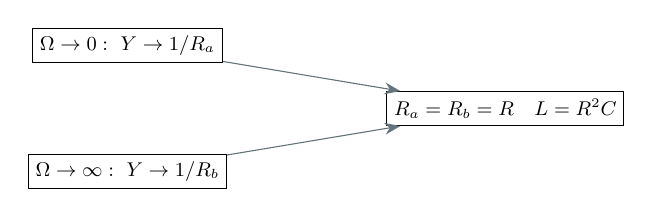
\begin{tikzpicture}[scale=.8,transform shape]
\node[draw] (lo) at (0,1) {$\Omega\to0:\ Y\to1/R_a$};\node[draw] (hi) at (0,-1) {$\Omega\to\infty:\ Y\to1/R_b$};\node[draw,align=center] (m) at (6,0) {$R_a=R_b=R$\quad $L=R^2C$};\draw[axis] (lo)--(m);\draw[axis] (hi)--(m);
\end{tikzpicture}
\figcaption{变图电试4.3V5\quad 低、高频两端确定相同电阻，再由中间频率的导纳关系匹配储能元件}
\end{minipage}\end{center}

\Needspace{20\baselineskip}
\item 匹配且零初态，输入改为斜坡电压$\mathcal E(t)=\alpha t$，$t\ge0$，求两支路电流。
\textbf{解：}变图电试4.3V6对$\tau\dot i_L+i_L=\alpha t/R$用积分因子，得$i_L=(\alpha/R)[t-\tau(1-e^{-t/\tau})]$。电容状态满足同一时间常数，$v_C/R=i_L$，所以$i_C=\alpha t/R-i_L=(\alpha\tau/R)(1-e^{-t/\tau})$。两者相加为$\alpha t/R$，即使输入不周期也成立。电感支路长期随斜坡增加，电容支路则趋于恒定电流$\alpha C$，与电容最终近似线性升压相容。
\begin{center}\begin{minipage}{.98\linewidth}\centering
\begin{tikzpicture}[scale=.8,transform shape]
\draw[axis] (0,0)--(10.7,0) node[right] {$t/\tau$};
\draw[axis] (0,0)--(0,3.2) node[above] {$iR/(\alpha\tau)$};\foreach \y/\lab in {0/0,1.3/2,2.6/4}{\draw[thin] (0,\y)--(-.08,\y) node[left] {$\lab$};}
\node[above] at (5,3.5) {非周期斜坡输入下，两支路总和为横坐标};
\draw[traj] plot coordinates {(0.000000000,0.000000000) (0.083333333,0.000556480) (0.166666667,0.002195536) (0.250000000,0.004872987) (0.333333333,0.008546455) (0.416666667,0.013175292) (0.500000000,0.018720509) (0.583333333,0.025144709) (0.666666667,0.032412019) (0.750000000,0.040488031) (0.833333333,0.049339743) (0.916666667,0.058935497) (1.000000000,0.069244929) (1.083333333,0.080238913) (1.166666667,0.091889511) (1.250000000,0.104169929) (1.333333333,0.117054461) (1.416666667,0.130518454) (1.500000000,0.144538259) (1.583333333,0.159091195) (1.666666667,0.174155502) (1.750000000,0.189710313) (1.833333333,0.205735609) (1.916666667,0.222212189) (2.000000000,0.239121637) (2.083333333,0.256446286) (2.166666667,0.274169193) (2.250000000,0.292274104) (2.333333333,0.310745429) (2.416666667,0.329568215) (2.500000000,0.348728118) (2.583333333,0.368211381) (2.666666667,0.388004806) (2.750000000,0.408095737) (2.833333333,0.428472032) (2.916666667,0.449122044) (3.000000000,0.470034604) (3.083333333,0.491198996) (3.166666667,0.512604944) (3.250000000,0.534242589) (3.333333333,0.556102475) (3.416666667,0.578175533) (3.500000000,0.600453063) (3.583333333,0.622926721) (3.666666667,0.645588502) (3.750000000,0.668430728) (3.833333333,0.691446037) (3.916666667,0.714627364) (4.000000000,0.737967934) (4.083333333,0.761461248) (4.166666667,0.785101073) (4.250000000,0.808881429) (4.333333333,0.832796582) (4.416666667,0.856841030) (4.500000000,0.881009496) (4.583333333,0.905296920) (4.666666667,0.929698446) (4.750000000,0.954209418) (4.833333333,0.978825370) (4.916666667,1.003542016) (5.000000000,1.028355249) (5.083333333,1.053261126) (5.166666667,1.078255866) (5.250000000,1.103335842) (5.333333333,1.128497577) (5.416666667,1.153737733) (5.500000000,1.179053110) (5.583333333,1.204440638) (5.666666667,1.229897373) (5.750000000,1.255420491) (5.833333333,1.281007281) (5.916666667,1.306655147) (6.000000000,1.332361594) (6.083333333,1.358124234) (6.166666667,1.383940771) (6.250000000,1.409809007) (6.333333333,1.435726832) (6.416666667,1.461692221) (6.500000000,1.487703235) (6.583333333,1.513758011) (6.666666667,1.539854762) (6.750000000,1.565991777) (6.833333333,1.592167411) (6.916666667,1.618380089) (7.000000000,1.644628299) (7.083333333,1.670910591) (7.166666667,1.697225574) (7.250000000,1.723571913) (7.333333333,1.749948330) (7.416666667,1.776353596) (7.500000000,1.802786535) (7.583333333,1.829246016) (7.666666667,1.855730958) (7.750000000,1.882240320) (7.833333333,1.908773106) (7.916666667,1.935328360) (8.000000000,1.961905165) (8.083333333,1.988502642) (8.166666667,2.015119947) (8.250000000,2.041756271) (8.333333333,2.068410838) (8.416666667,2.095082903) (8.500000000,2.121771752) (8.583333333,2.148476700) (8.666666667,2.175197090) (8.750000000,2.201932292) (8.833333333,2.228681702) (8.916666667,2.255444739) (9.000000000,2.282220848) (9.083333333,2.309009494) (9.166666667,2.335810167) (9.250000000,2.362622376) (9.333333333,2.389445649) (9.416666667,2.416279535) (9.500000000,2.443123602) (9.583333333,2.469977433) (9.666666667,2.496840630) (9.750000000,2.523712811) (9.833333333,2.550593610) (9.916666667,2.577482673) (10.000000000,2.604379666)};
\draw[dashed,thick,color=warm] plot coordinates {(0.000000000,0.000000000) (0.083333333,0.026526853) (0.166666667,0.051971130) (0.250000000,0.076377013) (0.333333333,0.099786879) (0.416666667,0.122241375) (0.500000000,0.143779491) (0.583333333,0.164438625) (0.666666667,0.184254648) (0.750000000,0.203261969) (0.833333333,0.221493590) (0.916666667,0.238981170) (1.000000000,0.255755071) (1.083333333,0.271844421) (1.166666667,0.287277155) (1.250000000,0.302080071) (1.333333333,0.316278873) (1.416666667,0.329898213) (1.500000000,0.342961741) (1.583333333,0.355492139) (1.666666667,0.367511164) (1.750000000,0.379039687) (1.833333333,0.390097725) (1.916666667,0.400704478) (2.000000000,0.410878363) (2.083333333,0.420637047) (2.166666667,0.429997474) (2.250000000,0.438975896) (2.333333333,0.447587904) (2.416666667,0.455848452) (2.500000000,0.463771882) (2.583333333,0.471371953) (2.666666667,0.478661860) (2.750000000,0.485654263) (2.833333333,0.492361301) (2.916666667,0.498794622) (3.000000000,0.504965396) (3.083333333,0.510884337) (3.166666667,0.516561723) (3.250000000,0.522007411) (3.333333333,0.527230858) (3.416666667,0.532241133) (3.500000000,0.537046937) (3.583333333,0.541656613) (3.666666667,0.546078165) (3.750000000,0.550319272) (3.833333333,0.554387296) (3.916666667,0.558289303) (4.000000000,0.562032066) (4.083333333,0.565622085) (4.166666667,0.569065594) (4.250000000,0.572368571) (4.333333333,0.575536751) (4.416666667,0.578575637) (4.500000000,0.581490504) (4.583333333,0.584286414) (4.666666667,0.586968221) (4.750000000,0.589540582) (4.833333333,0.592007964) (4.916666667,0.594374650) (5.000000000,0.596644751) (5.083333333,0.598822208) (5.166666667,0.600910801) (5.250000000,0.602914158) (5.333333333,0.604835757) (5.416666667,0.606678934) (5.500000000,0.608446890) (5.583333333,0.610142695) (5.666666667,0.611769293) (5.750000000,0.613329509) (5.833333333,0.614826052) (5.916666667,0.616261520) (6.000000000,0.617638406) (6.083333333,0.618959100) (6.166666667,0.620225896) (6.250000000,0.621440993) (6.333333333,0.622606502) (6.416666667,0.623724445) (6.500000000,0.624796765) (6.583333333,0.625825323) (6.666666667,0.626811904) (6.750000000,0.627758223) (6.833333333,0.628665922) (6.916666667,0.629536577) (7.000000000,0.630371701) (7.083333333,0.631172742) (7.166666667,0.631941093) (7.250000000,0.632678087) (7.333333333,0.633385003) (7.416666667,0.634063070) (7.500000000,0.634713465) (7.583333333,0.635337317) (7.666666667,0.635935709) (7.750000000,0.636509680) (7.833333333,0.637060228) (7.916666667,0.637588307) (8.000000000,0.638094835) (8.083333333,0.638580691) (8.166666667,0.639046719) (8.250000000,0.639493729) (8.333333333,0.639922495) (8.416666667,0.640333764) (8.500000000,0.640728248) (8.583333333,0.641106633) (8.666666667,0.641469576) (8.750000000,0.641817708) (8.833333333,0.642151631) (8.916666667,0.642471928) (9.000000000,0.642779152) (9.083333333,0.643073839) (9.166666667,0.643356499) (9.250000000,0.643627624) (9.333333333,0.643887684) (9.416666667,0.644137131) (9.500000000,0.644376398) (9.583333333,0.644605900) (9.666666667,0.644826036) (9.750000000,0.645037189) (9.833333333,0.645239724) (9.916666667,0.645433993) (10.000000000,0.645620334)};
\node[below] at (0,-.12) {$0$};
\node[below] at (5,-.12) {$2.5$};
\node[below] at (10,-.12) {$5$};
\end{tikzpicture}
\figcaption{变图电试4.3V6\quad 非周期斜坡输入下，两支路总和为横坐标}
\end{minipage}\end{center}

\Needspace{20\baselineskip}
\item 匹配时输入为单频电压，峰值$E_a$，求两个电阻的平均耗散功率及其分配。
\textbf{解：}变图电试4.3V7记$\nu=\Omega RC=\Omega L/R$。两支路电流峰值分别为$E_a/[R\sqrt{1+\nu^2}]$与$E_a\nu/[R\sqrt{1+\nu^2}]$，电阻功率用峰值平方乘$R/2$，得到$P_L=E_a^2/[2R(1+\nu^2)]$、$P_C=E_a^2\nu^2/[2R(1+\nu^2)]$。两者之比为$1:\nu^2$，总和恒为$E_a^2/(2R)$，等于端口有功输入。频率改变只改变内部两电阻的耗散分配，平均储能变化在一个周期内为零。
\begin{center}\begin{minipage}{.98\linewidth}\centering
\begin{tikzpicture}[scale=.8,transform shape]
\draw[axis] (0,0)--(10.7,0) node[right] {$\nu=\Omega RC$};
\draw[axis] (0,0)--(0,3.2) node[above] {$2RP/E_a^2$};\foreach \y/\lab in {0/0,1.4/0.5,2.8/1}{\draw[thin] (0,\y)--(-.08,\y) node[left] {$\lab$};}
\node[above] at (5,3.5) {两个电阻的平均耗散份额，实线RL、虚线RC};
\draw[traj] plot coordinates {(0.125000000,2.793017456) (0.207291667,2.780880961) (0.289583333,2.762928787) (0.371875000,2.739386787) (0.454166667,2.710544502) (0.536458333,2.676746512) (0.618750000,2.638382577) (0.701041667,2.595877081) (0.783333333,2.549678255) (0.865625000,2.500247653) (0.947916667,2.448050272) (1.030208333,2.393545619) (1.112500000,2.337179942) (1.194791667,2.279379768) (1.277083333,2.220546777) (1.359375000,2.161053996) (1.441666667,2.101243236) (1.523958333,2.041423635) (1.606250000,1.981871187) (1.688541667,1.922829077) (1.770833333,1.864508671) (1.853125000,1.807091017) (1.935416667,1.750728710) (2.017708333,1.695547999) (2.100000000,1.641651032) (2.182291667,1.589118167) (2.264583333,1.538010253) (2.346875000,1.488370857) (2.429166667,1.440228379) (2.511458333,1.393598038) (2.593750000,1.348483708) (2.676041667,1.304879601) (2.758333333,1.262771784) (2.840625000,1.222139549) (2.922916667,1.182956623) (3.005208333,1.145192241) (3.087500000,1.108812086) (3.169791667,1.073779104) (3.252083333,1.040054211) (3.334375000,1.007596898) (3.416666667,0.976365750) (3.498958333,0.946318876) (3.581250000,0.917414284) (3.663541667,0.889610177) (3.745833333,0.862865209) (3.828125000,0.837138686) (3.910416667,0.812390732) (3.992708333,0.788582414) (4.075000000,0.765675846) (4.157291667,0.743634257) (4.239583333,0.722422049) (4.321875000,0.702004827) (4.404166667,0.682349421) (4.486458333,0.663423892) (4.568750000,0.645197527) (4.651041667,0.627640831) (4.733333333,0.610725503) (4.815625000,0.594424418) (4.897916667,0.578711595) (4.980208333,0.563562163) (5.062500000,0.548952334) (5.144791667,0.534859363) (5.227083333,0.521261510) (5.309375000,0.508138006) (5.391666667,0.495469015) (5.473958333,0.483235593) (5.556250000,0.471419657) (5.638541667,0.460003943) (5.720833333,0.448971974) (5.803125000,0.438308023) (5.885416667,0.427997081) (5.967708333,0.418024822) (6.050000000,0.408377574) (6.132291667,0.399042289) (6.214583333,0.390006509) (6.296875000,0.381258344) (6.379166667,0.372786442) (6.461458333,0.364579963) (6.543750000,0.356628555) (6.626041667,0.348922331) (6.708333333,0.341451848) (6.790625000,0.334208081) (6.872916667,0.327182407) (6.955208333,0.320366585) (7.037500000,0.313752735) (7.119791667,0.307333324) (7.202083333,0.301101148) (7.284375000,0.295049313) (7.366666667,0.289171226) (7.448958333,0.283460576) (7.531250000,0.277911323) (7.613541667,0.272517682) (7.695833333,0.267274114) (7.778125000,0.262175315) (7.860416667,0.257216200) (7.942708333,0.252391898) (8.025000000,0.247697738) (8.107291667,0.243129243) (8.189583333,0.238682120) (8.271875000,0.234352247) (8.354166667,0.230135673) (8.436458333,0.226028604) (8.518750000,0.222027398) (8.601041667,0.218128558) (8.683333333,0.214328726) (8.765625000,0.210624675) (8.847916667,0.207013305) (8.930208333,0.203491635) (9.012500000,0.200056802) (9.094791667,0.196706049) (9.177083333,0.193436728) (9.259375000,0.190246289) (9.341666667,0.187132280) (9.423958333,0.184092338) (9.506250000,0.181124191) (9.588541667,0.178225650) (9.670833333,0.175394607) (9.753125000,0.172629031) (9.835416667,0.169926965) (9.917708333,0.167286521) (10.000000000,0.164705882)};
\draw[dashed,thick,color=warm] plot coordinates {(0.125000000,0.006982544) (0.207291667,0.019119039) (0.289583333,0.037071213) (0.371875000,0.060613213) (0.454166667,0.089455498) (0.536458333,0.123253488) (0.618750000,0.161617423) (0.701041667,0.204122919) (0.783333333,0.250321745) (0.865625000,0.299752347) (0.947916667,0.351949728) (1.030208333,0.406454381) (1.112500000,0.462820058) (1.194791667,0.520620232) (1.277083333,0.579453223) (1.359375000,0.638946004) (1.441666667,0.698756764) (1.523958333,0.758576365) (1.606250000,0.818128813) (1.688541667,0.877170923) (1.770833333,0.935491329) (1.853125000,0.992908983) (1.935416667,1.049271290) (2.017708333,1.104452001) (2.100000000,1.158348968) (2.182291667,1.210881833) (2.264583333,1.261989747) (2.346875000,1.311629143) (2.429166667,1.359771621) (2.511458333,1.406401962) (2.593750000,1.451516292) (2.676041667,1.495120399) (2.758333333,1.537228216) (2.840625000,1.577860451) (2.922916667,1.617043377) (3.005208333,1.654807759) (3.087500000,1.691187914) (3.169791667,1.726220896) (3.252083333,1.759945789) (3.334375000,1.792403102) (3.416666667,1.823634250) (3.498958333,1.853681124) (3.581250000,1.882585716) (3.663541667,1.910389823) (3.745833333,1.937134791) (3.828125000,1.962861314) (3.910416667,1.987609268) (3.992708333,2.011417586) (4.075000000,2.034324154) (4.157291667,2.056365743) (4.239583333,2.077577951) (4.321875000,2.097995173) (4.404166667,2.117650579) (4.486458333,2.136576108) (4.568750000,2.154802473) (4.651041667,2.172359169) (4.733333333,2.189274497) (4.815625000,2.205575582) (4.897916667,2.221288405) (4.980208333,2.236437837) (5.062500000,2.251047666) (5.144791667,2.265140637) (5.227083333,2.278738490) (5.309375000,2.291861994) (5.391666667,2.304530985) (5.473958333,2.316764407) (5.556250000,2.328580343) (5.638541667,2.339996057) (5.720833333,2.351028026) (5.803125000,2.361691977) (5.885416667,2.372002919) (5.967708333,2.381975178) (6.050000000,2.391622426) (6.132291667,2.400957711) (6.214583333,2.409993491) (6.296875000,2.418741656) (6.379166667,2.427213558) (6.461458333,2.435420037) (6.543750000,2.443371445) (6.626041667,2.451077669) (6.708333333,2.458548152) (6.790625000,2.465791919) (6.872916667,2.472817593) (6.955208333,2.479633415) (7.037500000,2.486247265) (7.119791667,2.492666676) (7.202083333,2.498898852) (7.284375000,2.504950687) (7.366666667,2.510828774) (7.448958333,2.516539424) (7.531250000,2.522088677) (7.613541667,2.527482318) (7.695833333,2.532725886) (7.778125000,2.537824685) (7.860416667,2.542783800) (7.942708333,2.547608102) (8.025000000,2.552302262) (8.107291667,2.556870757) (8.189583333,2.561317880) (8.271875000,2.565647753) (8.354166667,2.569864327) (8.436458333,2.573971396) (8.518750000,2.577972602) (8.601041667,2.581871442) (8.683333333,2.585671274) (8.765625000,2.589375325) (8.847916667,2.592986695) (8.930208333,2.596508365) (9.012500000,2.599943198) (9.094791667,2.603293951) (9.177083333,2.606563272) (9.259375000,2.609753711) (9.341666667,2.612867720) (9.423958333,2.615907662) (9.506250000,2.618875809) (9.588541667,2.621774350) (9.670833333,2.624605393) (9.753125000,2.627370969) (9.835416667,2.630073035) (9.917708333,2.632713479) (10.000000000,2.635294118)};
\node[below] at (0,-.12) {$0$极限};
\node[below] at (2.5,-.12) {$1$};
\node[below] at (10,-.12) {$4$};
\end{tikzpicture}
\figcaption{变图电试4.3V7\quad 两个电阻的平均耗散份额，实线RL、虚线RC}
\end{minipage}\end{center}

\Needspace{20\baselineskip}
\item 令$L=(1+\epsilon)R^2C$，$|\epsilon|\ll1$。求总导纳偏离$1/R$的一阶项及最大相对偏差频率。
\textbf{解：}变图电试4.3V8记$\nu=\Omega RC$，把主解的通分结果按$\epsilon$展开，$Y-1/R=-j\nu\epsilon/[R(1+j\nu)^2]+O(\epsilon^2/R)$。一阶相对偏差的模为$R|\delta Y|=|\epsilon|\nu/(1+\nu^2)$。对$\nu$求导得$(1-\nu^2)/(1+\nu^2)^2$，所以最大值为$|\epsilon|/2$，出现在$\Omega=1/(RC)$。低频和高频的端口偏差都趋零，中间频段最能显出时间常数失配。
\begin{center}\begin{minipage}{.98\linewidth}\centering
\begin{tikzpicture}[scale=.8,transform shape]
\draw[axis] (0,0)--(10.7,0) node[right] {$\nu=\Omega RC$};
\draw[axis] (0,0)--(0,3.2) node[above] {$R|\delta Y|/|\epsilon|$};\foreach \y/\lab in {0/0,1.375/0.25,2.75/0.5}{\draw[thin] (0,\y)--(-.08,\y) node[left] {$\lab$};}
\node[above] at (5,3.5) {小失配的一阶相对导纳偏差，峰值在$\nu=1$};
\draw[traj] plot coordinates {(0.125000000,0.274314214) (0.207291667,0.452927710) (0.289583333,0.628648529) (0.371875000,0.800414577) (0.454166667,0.967244898) (0.536458333,1.128256621) (0.618750000,1.282677958) (0.701041667,1.429856997) (0.783333333,1.569266259) (0.865625000,1.700503259) (0.947916667,1.823287443) (1.030208333,1.937454077) (1.112500000,2.042945681) (1.194791667,2.139801676) (1.277083333,2.228146862) (1.359375000,2.308179324) (1.441666667,2.380158260) (1.523958333,2.444392154) (1.606250000,2.501227610) (1.688541667,2.551039082) (1.770833333,2.594219653) (1.853125000,2.631172925) (1.935416667,2.662306055) (2.017708333,2.688023899) (2.100000000,2.708724203) (2.182291667,2.724793761) (2.264583333,2.736605445) (2.346875000,2.744515993) (2.429166667,2.748864463) (2.511458333,2.749971248) (2.593750000,2.748137557) (2.676041667,2.743645286) (2.758333333,2.736757182) (2.840625000,2.727717266) (2.922916667,2.716751423) (3.005208333,2.704068138) (3.087500000,2.689859319) (3.169791667,2.674301186) (3.252083333,2.657555186) (3.334375000,2.639768927) (3.416666667,2.621077102) (3.498958333,2.601602393) (3.581250000,2.581456354) (3.663541667,2.560740247) (3.745833333,2.539545849) (3.828125000,2.517956204) (3.910416667,2.496046345) (3.992708333,2.473883953) (4.075000000,2.451529984) (4.157291667,2.429039250) (4.239583333,2.406460947) (4.321875000,2.383839159) (4.404166667,2.361213309) (4.486458333,2.338618580) (4.568750000,2.316086301) (4.651041667,2.293644300) (4.733333333,2.271317228) (4.815625000,2.249126856) (4.897916667,2.227092343) (4.980208333,2.205230484) (5.062500000,2.183555937) (5.144791667,2.162081423) (5.227083333,2.140817918) (5.309375000,2.119774820) (5.391666667,2.098960105) (5.473958333,2.078380466) (5.556250000,2.058041441) (5.638541667,2.037947530) (5.720833333,2.018102301) (5.803125000,1.998508481) (5.885416667,1.979168049) (5.967708333,1.960082310) (6.050000000,1.941251969) (6.132291667,1.922677194) (6.214583333,1.904357675) (6.296875000,1.886292677) (6.379166667,1.868481091) (6.461458333,1.850921472) (6.543750000,1.833612082) (6.626041667,1.816550926) (6.708333333,1.799735781) (6.790625000,1.783164231) (6.872916667,1.766833685) (6.955208333,1.750741409) (7.037500000,1.734884542) (7.119791667,1.719260117) (7.202083333,1.703865080) (7.284375000,1.688696302) (7.366666667,1.673750597) (7.448958333,1.659024731) (7.531250000,1.644515439) (7.613541667,1.630219426) (7.695833333,1.616133387) (7.778125000,1.602254005) (7.860416667,1.588577968) (7.942708333,1.575101965) (8.025000000,1.561822701) (8.107291667,1.548736899) (8.189583333,1.535841299) (8.271875000,1.523132672) (8.354166667,1.510607816) (8.436458333,1.498263561) (8.518750000,1.486096773) (8.601041667,1.474104355) (8.683333333,1.462283247) (8.765625000,1.450630434) (8.847916667,1.439142940) (8.930208333,1.427817834) (9.012500000,1.416652228) (9.094791667,1.405643280) (9.177083333,1.394788195) (9.259375000,1.384084221) (9.341666667,1.373528654) (9.423958333,1.363118837) (9.506250000,1.352852160) (9.588541667,1.342726058) (9.670833333,1.332738012) (9.753125000,1.322885552) (9.835416667,1.313166251) (9.917708333,1.303577727) (10.000000000,1.294117647)};
\node[below] at (0,-.12) {$0$极限};
\node[below] at (2.5,-.12) {$1$};
\node[below] at (10,-.12) {$4$};
\end{tikzpicture}
\figcaption{变图电试4.3V8\quad 小失配的一阶相对导纳偏差，峰值在$\nu=1$}
\end{minipage}\end{center}
\end{enumerate}

\Needspace{13\baselineskip}

\pdfbookmark[2]{第 4 题 双行CLC网络的复阻抗和功率因数}{q4}

\section*{第 4 题\quad 双行CLC网络的复阻抗和功率因数}\label{q:4}


如图，两条水平支路各依次由电容$C$、电感$L$、电容$C$连接而成；四列上下对应结点之间均接电阻$R$。以左下结点$A$和右上结点$B$为端口。
\begin{enumerate}
\item 求角频率$\omega$下的端口复阻抗$Z$。
\item 当$\omega L=1/(\omega C)=R$时，求$|Z|$和功率因数，说明电流相位。
\end{enumerate}
所有同名元件参数相同；用电流从$A$流入、从$B$流出的方向定义端口电压。


\begin{center}\begin{minipage}{.98\linewidth}\centering
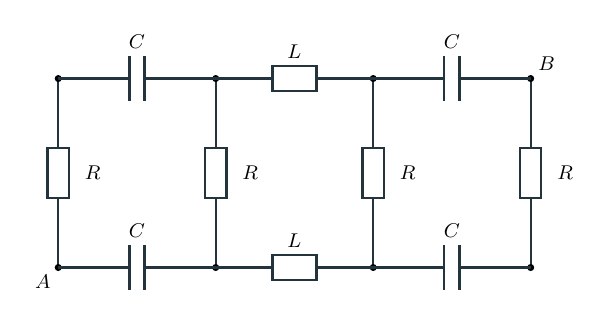
\begin{tikzpicture}[scale=.8,transform shape]

\foreach \x in {0,2.5,5,7.5}{
\draw[object] (\x,0)--(\x,1.1);
\draw[object] ({\x-.17},1.1) rectangle ({\x+.17},1.9);
\draw[object] (\x,1.9)--(\x,3);
\node[right] at ({\x+.3},1.5) {$R$};
\fill (\x,0) circle (1.6pt);\fill (\x,3) circle (1.6pt);}
\foreach \y in {0,3}{
\foreach \a/\b in {0/2.5,5/7.5}{
\pgfmathsetmacro{\m}{(\a+\b)/2}
\draw[object] (\a,\y)--({\m-.12},\y);
\draw[object] ({\m+.12},\y)--(\b,\y);
\draw[object] ({\m-.12},{\y-.35})--({\m-.12},{\y+.35});
\draw[object] ({\m+.12},{\y-.35})--({\m+.12},{\y+.35});
\node[above] at (\m,{\y+.35}) {$C$};}
\draw[object] (2.5,\y)--(3.4,\y);
\draw[object] (3.4,{\y-.2}) rectangle (4.1,{\y+.2});
\draw[object] (4.1,\y)--(5,\y);\node[above] at (3.75,{\y+.2}) {$L$};}
\node[below left] at (0,0) {$A$};\node[above right] at (7.5,3) {$B$};

\end{tikzpicture}
\figcaption{图电试4.4\quad 上下均为CLC，四列竖直电阻相同；端口在对角两端。}
\end{minipage}\end{center}

\Needspace{8\baselineskip}

\pdfbookmark[3]{题型定位}{q4-h0}

\subsection*{题型定位}

利用端口交换对称性求交流梯形网络的阻抗。先用中心反对称电势确定对应支路的复电流关系，再以结点守恒和同端点路径电压求两类电流。端口电压沿实际支路相加，阻抗实部与四个电阻耗散相对应，阻抗辐角给电流超前或滞后。

\Needspace{8\baselineskip}

\pdfbookmark[3]{知识点}{q4-h1}

\subsection*{知识点}

线性网络的端口激励可取正负一半电势，交换端口的对称变换对应电势反号。复电流箭头规定代数正方向，复数幅度保留相位。KCL先给两电感各承担端口电流一半，KVL再给外、内电阻电流比例。复阻抗有理化后分别求实部、虚部、模和相位；有效值相量的有功功率为电流模平方乘阻抗实部。

\Needspace{8\baselineskip}

\pdfbookmark[3]{物理图像}{q4-h2}

\subsection*{物理图像}

题图两行$C-L-C$和四列电阻共同组成网络，解图电试4.4A把两类竖直电流与上下电感电流一并标出，$A$到$P$的两条路径用于同一电势差比较。图B的阻抗位于第四象限，水平长度$3R/8$、向下长度$5R/8$。图C保持元件参数改变频率，显示实部始终为正、电抗由容性变为感性，说明特殊频率只取其中一个点。

\Needspace{8\baselineskip}

\pdfbookmark[3]{解题入口}{q4-h3}

\subsection*{解题入口}

在空白网络先找中心旋转对应点，以$\pm V/2$端口电势说明对应电流关系。内侧下结点KCL给$I_1-I_2=I/2$，左矩形两条路径的KVL给第二个方程。求比例后按图A上方路径逐段相加端口电压，最后将四个电阻各自的热功率相加，得到端口有功功率。

\Needspace{8\baselineskip}

\pdfbookmark[3]{标准解法}{q4-h4}

\subsection*{标准解法}


图电试4.4关于中心旋转$180^\circ$后互换端口。将端口电势取为$+V/2,-V/2$，由线性与唯一性，对应结点电势互为相反数；对应支路的代数电流据此配对。
\begin{center}\begin{minipage}{.98\linewidth}\centering
\begin{tikzpicture}[scale=.8,transform shape]

\foreach \x in {0,2.5,5,7.5}{
\draw[object] (\x,0)--(\x,1.1);
\draw[object] ({\x-.17},1.1) rectangle ({\x+.17},1.9);
\draw[object] (\x,1.9)--(\x,3);
\node[right] at ({\x+.3},1.5) {$R$};
\fill (\x,0) circle (1.6pt);\fill (\x,3) circle (1.6pt);}
\foreach \y in {0,3}{
\foreach \a/\b in {0/2.5,5/7.5}{
\pgfmathsetmacro{\m}{(\a+\b)/2}
\draw[object] (\a,\y)--({\m-.12},\y);
\draw[object] ({\m+.12},\y)--(\b,\y);
\draw[object] ({\m-.12},{\y-.35})--({\m-.12},{\y+.35});
\draw[object] ({\m+.12},{\y-.35})--({\m+.12},{\y+.35});
\node[above] at (\m,{\y+.35}) {$C$};}
\draw[object] (2.5,\y)--(3.4,\y);
\draw[object] (3.4,{\y-.2}) rectangle (4.1,{\y+.2});
\draw[object] (4.1,\y)--(5,\y);\node[above] at (3.75,{\y+.2}) {$L$};}
\node[below left] at (0,0) {$A$};\node[above right] at (7.5,3) {$B$};

\draw[motion] (-.6,.5)--(-.6,2.5) node[midway,left] {$I_1$};
\draw[motion] (8.9,.5)--(8.9,2.5) node[midway,right] {$I_1$};
\draw[force] (2,2.5)--(2,.5) node[midway,left] {$I_2$};
\draw[force] (4.5,2.5)--(4.5,.5) node[midway,left] {$I_2$};
\draw[motion] (3.2,-.7)--(4.4,-.7) node[midway,below] {$I/2$};
\draw[motion] (3.2,3.8)--(4.4,3.8) node[midway,above] {$I/2$};
\draw[motion] (-1.4,0)--(-.2,0) node[midway,above] {$I$};
\draw[motion] (7.7,3)--(8.9,3) node[midway,above] {$I$};
\node[below] at (2.5,0) {$P$};
\node at (3.75,-2) {箭头为相量的代数正方向};

\end{tikzpicture}
\figcaption{解图电试4.4A\quad 对称性配对竖边电流，P点守恒给出每个电感电流I/2。}
\end{minipage}\end{center}
解图电试4.4A中，左、右外侧竖直电阻电流均向上记为$\widetilde I_1$，两条内侧竖直电阻电流均向下记为$\widetilde I_2$；各相量箭头规定代数参考方向，瞬时电流由求得的复振幅和时间因子取实部得到。端口总电流为$\widetilde I$。

对称旋转把左外电阻与右外电阻互换，也把两个内电阻互换；端口电势交换后同时反号，选定支路方向的电流便有图中相同的复振幅。外侧与内侧仍是两组独立未知量。沿对应横向支路，电流由所在结点的流入、流出确定。

左下结点向右流入第一个电容的电流为$\widetilde I-\widetilde I_1$。在其右方下侧结点$P$，从上方电阻又流入$\widetilde I_2$，向右通过下电感的电流则为$\widetilde I_1-\widetilde I_2$。故
\[
(\widetilde I-\widetilde I_1)+\widetilde I_2
=\widetilde I_1-\widetilde I_2,
\qquad
\boxed{\widetilde I_1-\widetilde I_2=\widetilde I/2}.
\]
将结点式整理为$\widetilde I=2(\widetilde I_1-\widetilde I_2)$，它在求任何阻抗前就固定了中段横向电流。上下两个电感均流过$\widetilde I/2$。令$Z_c=1/(\mathrm j\omega C)$，沿左侧矩形的两条路径比较$A$到$P$的电压降：
\[
\widetilde I_1(R+Z_c)+\widetilde I_2R
=(\widetilde I-\widetilde I_1)Z_c.
\]
用$\widetilde I_2=\widetilde I_1-\widetilde I/2$消元得
\[
\boxed{\frac{\widetilde I_1}{\widetilde I}
=\frac{R/2+Z_c}{2(R+Z_c)}},\qquad
\frac{\widetilde I_2}{\widetilde I}
=-\frac{R}{4(R+Z_c)}.
\]
具体消元时左端成为$\widetilde I_1(2R+Z_c)-\widetilde IR/2$，移去右端的$-\widetilde I_1Z_c$后有$2(R+Z_c)\widetilde I_1=\widetilde I(R/2+Z_c)$；再减去$\widetilde I/2$得到内侧电流。第二式实部为负，说明相应同相分量沿图中向下方向的反向。

端口电压沿左竖电阻、左上电容、上电感、右上电容的路径相加：
\[
\widetilde V=\widetilde I_1(R+Z_c)
+\frac{\widetilde I}{2}\mathrm j\omega L
+(\widetilde I-\widetilde I_1)Z_c.
\]
因此
\[
Z=\frac{R/2+Z_c}{2}
+\frac{\mathrm j\omega L}{2}
+Z_c\left[1-\frac{R/2+Z_c}{2(R+Z_c)}\right].
\]
这里第一项来自左外电阻与左上电容，第二项来自上电感，末项来自右上电容。将端电流提出后，把公共分母$R+Z_c=R-j/(\omega C)$乘以共轭。利用$1/(R+Z_c)=[R+j/(\omega C)]/[R^2+1/(\omega^2C^2)]$分开实、虚部，再将$x=\omega RC$引入并有理化，可得
\[
\boxed{\operatorname{Re}Z=
\frac{R(2+x^2)}{4(1+x^2)}},
\qquad
\boxed{\operatorname{Im}Z=
\frac{\omega L}{2}-\frac1{\omega C}
-\frac{R x}{4(1+x^2)}}.
\]
实部始终为正，来自四个电阻的耗散；电抗则由两种储能贡献共同决定。
\begin{center}\begin{minipage}{.98\linewidth}\centering
\begin{tikzpicture}[scale=.8,transform shape]

\draw[axis] (0,0)--(4.8,0) node[right] {$\operatorname{Re}Z$};
\draw[axis] (0,-4.4)--(0,1) node[above] {$\operatorname{Im}Z$};
\draw[force] (0,0)--(2.4,-4) node[midway,right] {$Z$};
\draw[guide] (2.4,0)--(2.4,-4)--(0,-4);
\node[above] at (2.4,0) {$3R/8$};\node[left] at (0,-4) {$-5R/8$};
\node[align=left] at (7,-1.8) {$|Z|=\sqrt{34}R/8$\\$\cos\phi=3/\sqrt{34}$\\电流超前端电压};

\end{tikzpicture}
\figcaption{解图电试4.4B\quad 特殊频率下阻抗在第四象限，有功实部仍为正。}
\end{minipage}\end{center}
\begin{center}\begin{minipage}{.98\linewidth}\centering
\begin{tikzpicture}[scale=.8,transform shape]
\draw[axis] (0,0)--(10.7,0) node[right] {$\omega/\omega_0$};
\draw[axis] (0,0)--(0,3.2) node[above] {$Z/R$};\foreach \y/\lab in {0.81/-1,2.61/1}{\draw[thin] (0,\y)--(-.08,\y) node[left] {$\lab$};}
\node[above] at (5,3.5) {实线电阻，虚线电抗；元件在$\omega_0$满足题设条件};
\draw[traj] plot coordinates {(1.666666667,2.115000000) (1.736111111,2.111988733) (1.805555556,2.108959732) (1.875000000,2.105919881) (1.944444444,2.102875648) (2.013888889,2.099833068) (2.083333333,2.096797753) (2.152777778,2.093774885) (2.222222222,2.090769231) (2.291666667,2.087785146) (2.361111111,2.084826590) (2.430555556,2.081897138) (2.500000000,2.079000000) (2.569444444,2.076138034) (2.638888889,2.073313767) (2.708333333,2.070529412) (2.777777778,2.067786885) (2.847222222,2.065087829) (2.916666667,2.062433628) (2.986111111,2.059825427) (3.055555556,2.057264151) (3.125000000,2.054750520) (3.194444444,2.052285068) (3.263888889,2.049868159) (3.333333333,2.047500000) (3.402777778,2.045180659) (3.472222222,2.042910075) (3.541666667,2.040688073) (3.611111111,2.038514377) (3.680555556,2.036388617) (3.750000000,2.034310345) (3.819444444,2.032279039) (3.888888889,2.030294118) (3.958333333,2.028354943) (4.027777778,2.026460833) (4.097222222,2.024611063) (4.166666667,2.022804878) (4.236111111,2.021041494) (4.305555556,2.019320104) (4.375000000,2.017639885) (4.444444444,2.016000000) (4.513888889,2.014399602) (4.583333333,2.012837838) (4.652777778,2.011313852) (4.722222222,2.009826790) (4.791666667,2.008375796) (4.861111111,2.006960022) (4.930555556,2.005578625) (5.000000000,2.004230769) (5.069444444,2.002915630) (5.138888889,2.001632391) (5.208333333,2.000380250) (5.277777778,1.999158416) (5.347222222,1.997966112) (5.416666667,1.996802575) (5.486111111,1.995667057) (5.555555556,1.994558824) (5.625000000,1.993477157) (5.694444444,1.992421356) (5.763888889,1.991390732) (5.833333333,1.990384615) (5.902777778,1.989402351) (5.972222222,1.988443299) (6.041666667,1.987506837) (6.111111111,1.986592357) (6.180555556,1.985699267) (6.250000000,1.984826990) (6.319444444,1.983974965) (6.388888889,1.983142645) (6.458333333,1.982329499) (6.527777778,1.981535009) (6.597222222,1.980758672) (6.666666667,1.980000000) (6.736111111,1.979258516) (6.805555556,1.978533759) (6.875000000,1.977825279) (6.944444444,1.977132640) (7.013888889,1.976455418) (7.083333333,1.975793201) (7.152777778,1.975145590) (7.222222222,1.974512195) (7.291666667,1.973892640) (7.361111111,1.973286558) (7.430555556,1.972693594) (7.500000000,1.972113402) (7.569444444,1.971545647) (7.638888889,1.970990003) (7.708333333,1.970446154) (7.777777778,1.969913793) (7.847222222,1.969392623) (7.916666667,1.968882353) (7.986111111,1.968382703) (8.055555556,1.967893401) (8.125000000,1.967414181) (8.194444444,1.966944787) (8.263888889,1.966484968) (8.333333333,1.966034483) (8.402777778,1.965593095) (8.472222222,1.965160577) (8.541666667,1.964736706) (8.611111111,1.964321267) (8.680555556,1.963914050) (8.750000000,1.963514851) (8.819444444,1.963123474) (8.888888889,1.962739726) (8.958333333,1.962363420) (9.027777778,1.961994376) (9.097222222,1.961632417) (9.166666667,1.961277372) (9.236111111,1.960929075) (9.305555556,1.960587364) (9.375000000,1.960252082) (9.444444444,1.959923077) (9.513888889,1.959600199) (9.583333333,1.959283305) (9.652777778,1.958972254) (9.722222222,1.958666910) (9.791666667,1.958367140) (9.861111111,1.958072815) (9.930555556,1.957783809) (10.000000000,1.957500000)};
\draw[dashed,thick,color=warm] plot coordinates {(1.666666667,0.045000000) (1.736111111,0.124193368) (1.805555556,0.197983351) (1.875000000,0.266982567) (1.944444444,0.331715396) (2.013888889,0.392633182) (2.083333333,0.450126404) (2.152777778,0.504534500) (2.222222222,0.556153846) (2.291666667,0.605244303) (2.361111111,0.652034597) (2.430555556,0.696726789) (2.500000000,0.739500000) (2.569444444,0.780513531) (2.638888889,0.819909496) (2.708333333,0.857815045) (2.777777778,0.894344262) (2.847222222,0.929599776) (2.916666667,0.963674147) (2.986111111,0.996651058) (3.055555556,1.028606346) (3.125000000,1.059608888) (3.194444444,1.089721375) (3.263888889,1.119000992) (3.333333333,1.147500000) (3.402777778,1.175266258) (3.472222222,1.202343672) (3.541666667,1.228772598) (3.611111111,1.254590194) (3.680555556,1.279830729) (3.750000000,1.304525862) (3.819444444,1.328704889) (3.888888889,1.352394958) (3.958333333,1.375621268) (4.027777778,1.398407241) (4.097222222,1.420774678) (4.166666667,1.442743902) (4.236111111,1.464333880) (4.305555556,1.485562339) (4.375000000,1.506445865) (4.444444444,1.527000000) (4.513888889,1.547239321) (4.583333333,1.567177518) (4.652777778,1.586827461) (4.722222222,1.606201263) (4.791666667,1.625310336) (4.861111111,1.644165444) (4.930555556,1.662776746) (5.000000000,1.681153846) (5.069444444,1.699305825) (5.138888889,1.717241280) (5.208333333,1.734968360) (5.277777778,1.752494789) (5.347222222,1.769827901) (5.416666667,1.786974662) (5.486111111,1.803941693) (5.555555556,1.820735294) (5.625000000,1.837361464) (5.694444444,1.853825916) (5.763888889,1.870134098) (5.833333333,1.886291209) (5.902777778,1.902302210) (5.972222222,1.918171841) (6.041666667,1.933904634) (6.111111111,1.949504922) (6.180555556,1.964976852) (6.250000000,1.980324394) (6.319444444,1.995551355) (6.388888889,2.010661380) (6.458333333,2.025657967) (6.527777778,2.040544473) (6.597222222,2.055324119) (6.666666667,2.070000000) (6.736111111,2.084575090) (6.805555556,2.099052249) (6.875000000,2.113434226) (6.944444444,2.127723667) (7.013888889,2.141923119) (7.083333333,2.156035036) (7.152777778,2.170061780) (7.222222222,2.184005629) (7.291666667,2.197868778) (7.361111111,2.211653347) (7.430555556,2.225361379) (7.500000000,2.238994845) (7.569444444,2.252555652) (7.638888889,2.266045638) (7.708333333,2.279466580) (7.777777778,2.292820197) (7.847222222,2.306108149) (7.916666667,2.319332043) (7.986111111,2.332493433) (8.055555556,2.345593821) (8.125000000,2.358634664) (8.194444444,2.371617371) (8.263888889,2.384543306) (8.333333333,2.397413793) (8.402777778,2.410230112) (8.472222222,2.422993506) (8.541666667,2.435705178) (8.611111111,2.448366297) (8.680555556,2.460977995) (8.750000000,2.473541372) (8.819444444,2.486057494) (8.888888889,2.498527397) (8.958333333,2.510952087) (9.027777778,2.523332539) (9.097222222,2.535669702) (9.166666667,2.547964499) (9.236111111,2.560217824) (9.305555556,2.572430548) (9.375000000,2.584603518) (9.444444444,2.596737557) (9.513888889,2.608833464) (9.583333333,2.620892019) (9.652777778,2.632913980) (9.722222222,2.644900083) (9.791666667,2.656851048) (9.861111111,2.668767571) (9.930555556,2.680650334) (10.000000000,2.692500000)};
\node[below] at (1.6666666666666667,-.12) {$1/2$};
\node[below] at (3.3333333333333335,-.12) {$1$};
\node[below] at (10,-.12) {$3$};
\draw[dotted] (0,1.71)--(10,1.71);\node[left] at (0,1.71) {$0$};
\end{tikzpicture}
\figcaption{解图电试4.4C\quad 实线电阻，虚线电抗；元件在$\omega_0$满足题设条件}
\end{minipage}\end{center}
解图电试4.4C以元件固定、频率变化为例，同时画出端口实部与电抗。电阻实部介于$R/4$和$R/2$之间；低频主要为容性，高频主要为感性。题设频率对应横坐标1，位于容性一侧。

在题给$\omega L=1/(\omega C)=R$时，$x=1$。解图电试4.4B的阻抗点位于第四象限：
\[
\boxed{Z=\frac R8(3-5\mathrm j)},\qquad
\boxed{|Z|=\frac{\sqrt{34}}8R}.
\]
阻抗模由直角三角形的两直角边求得$R\sqrt{3^2+5^2}/8$，而相位保留虚部的负号。以端电压为相位参考，$\arg Z=-\arctan(5/3)$，所以电流超前电压$\arctan(5/3)$。功率因数为
\[
\boxed{\cos\phi=\frac{\operatorname{Re}Z}{|Z|}
=\frac3{\sqrt{34}}\approx0.5145}.
\]
这里功率因数取正的幅值，另说明超前；负电抗表示容性，有功功率仍为正。

四个电阻的耗散给出阻抗实部的能量表达。在该频率$\widetilde I_1/\widetilde I=(3-\mathrm j)/8$，
$\widetilde I_2/\widetilde I=(-1-\mathrm j)/8$，按有效值相量，
\[
P=2R|\widetilde I_1|^2+2R|\widetilde I_2|^2
=\frac{3R}{8}|\widetilde I|^2
=|\widetilde I|^2\operatorname{Re}Z.
\]
两类电阻的热功率相加，恰给端口实部系数$3/8$。


\Needspace{8\baselineskip}

\pdfbookmark[3]{关键洞察}{q4-h5}

\subsection*{关键洞察}

对称性将竖直支路分为外侧和内侧两类，电感电流为一半由具体KCL确定。电容电流分别按所在结点取$I_1$或$I-I_1$等组合。求得的电流比例与$L$无关，是该拓扑和成对相同元件共同给出的关系；$L$改变端口电抗。四个电阻的耗散使实部为正，负电抗则使电流超前，两种现象分别描述能量耗散与储能交换。

\Needspace{8\baselineskip}

\pdfbookmark[3]{易错点}{q4-h6}

\subsection*{易错点}

外侧$I_1$与内侧$I_2$保留各自的代数方向，按结点守恒决定组合。沿端口路径包括两个电容和一个电感，电流幅度各不相同。电容阻抗为$-j/(\omega C)$，有理化时连同负号一起运算。阻抗模用于电压电流有效值比，阻抗实部用于有功功率；相位由$\arg Z$确定，第四象限给电流超前。

\Needspace{8\baselineskip}

\pdfbookmark[3]{课堂讲解建议}{q4-h7}

\subsection*{课堂讲解建议}

先在空白图上连出旋转对应点，让学生说清外、内竖直支路为什么分别配对。标完电流后只写$P$点KCL，再分别沿两条$A-P$路径写电压，逐段标出相应的复电流及压降。让学生说明两电感各流过$I/2$与$L$数值的关系：这一比例已由成对支路的对称性和$P$点KCL确定，改变两只相同电感的$L$仍保留它。

求出一般阻抗后，要求先看量纲与实部正值，再代入特殊频率。在图B上同时标阻抗辐角和电流相对电压的超前角。另一组用两类电阻电流计算热功率，把实部系数$3/8$与每个电阻的实际耗散联系起来。最后结合图C讨论改变频率时容性与感性的转换。

\Needspace{8\baselineskip}

\pdfbookmark[3]{变式训练}{q4-h8}

\subsection*{变式训练}

\begin{enumerate}
\Needspace{20\baselineskip}
\item 给定$R,C,\omega$，调电感使端口功率因数为1，求所需$L$。
\textbf{解：}变图电试4.4V1要求$\Im Z=0$，故$\omega L/2=1/(\omega C)+R^2\omega C/[4(1+\omega^2R^2C^2)]$。解出$L=2/(\omega^2C)+R^2C/[2(1+\omega^2R^2C^2)]>0$。此时端口阻抗为实数$R(2+x^2)/[4(1+x^2)]$，电流与端电压同相。电感所需补偿既包括两个电容组合的电抗，也包括电阻支路分流带来的附加电抗项。
\begin{center}\begin{minipage}{.98\linewidth}\centering
\begin{tikzpicture}[scale=.8,transform shape]
\draw[axis] (0,0)--(10.7,0) node[right] {$x=\omega RC$};
\draw[axis] (0,0)--(0,3.2) node[above] {$L/(R^2C)$};\foreach \y/\lab in {0/0,1.2/10,2.4/20}{\draw[thin] (0,\y)--(-.08,\y) node[left] {$\lab$};}
\node[above] at (5,3.5) {固定频率与电容时，同相所需的归一化电感};
\draw[traj] plot coordinates {(1.000000000,2.721712538) (1.075000000,2.361901151) (1.150000000,2.070001218) (1.225000000,1.829898162) (1.300000000,1.629988083) (1.375000000,1.461743523) (1.450000000,1.318784378) (1.525000000,1.196260391) (1.600000000,1.090431296) (1.675000000,0.998375476) (1.750000000,0.917784066) (1.825000000,0.846813030) (1.900000000,0.783975264) (1.975000000,0.728060822) (2.050000000,0.678077187) (2.125000000,0.633204026) (2.200000000,0.592758559) (2.275000000,0.556168784) (2.350000000,0.522952586) (2.425000000,0.492701298) (2.500000000,0.465066667) (2.575000000,0.439750434) (2.650000000,0.416495957) (2.725000000,0.395081417) (2.800000000,0.375314291) (2.875000000,0.357026817) (2.950000000,0.340072260) (3.025000000,0.324321816) (3.100000000,0.309662034) (3.175000000,0.295992666) (3.250000000,0.283224855) (3.325000000,0.271279609) (3.400000000,0.260086506) (3.475000000,0.249582600) (3.550000000,0.239711477) (3.625000000,0.230422457) (3.700000000,0.221669900) (3.775000000,0.213412614) (3.850000000,0.205613339) (3.925000000,0.198238302) (4.000000000,0.191256831) (4.075000000,0.184641010) (4.150000000,0.178365393) (4.225000000,0.172406738) (4.300000000,0.166743779) (4.375000000,0.161357031) (4.450000000,0.156228605) (4.525000000,0.151342060) (4.600000000,0.146682256) (4.675000000,0.142235235) (4.750000000,0.137988109) (4.825000000,0.133928964) (4.900000000,0.130046770) (4.975000000,0.126331303) (5.050000000,0.122773077) (5.125000000,0.119363276) (5.200000000,0.116093700) (5.275000000,0.112956716) (5.350000000,0.109945204) (5.425000000,0.107052523) (5.500000000,0.104272470) (5.575000000,0.101599243) (5.650000000,0.099027413) (5.725000000,0.096551894) (5.800000000,0.094167919) (5.875000000,0.091871011) (5.950000000,0.089656970) (6.025000000,0.087521843) (6.100000000,0.085461915) (6.175000000,0.083473688) (6.250000000,0.081553864) (6.325000000,0.079699336) (6.400000000,0.077907171) (6.475000000,0.076174601) (6.550000000,0.074499008) (6.625000000,0.072877920) (6.700000000,0.071308996) (6.775000000,0.069790021) (6.850000000,0.068318896) (6.925000000,0.066893631) (7.000000000,0.065512342) (7.075000000,0.064173236) (7.150000000,0.062874615) (7.225000000,0.061614863) (7.300000000,0.060392446) (7.375000000,0.059205904) (7.450000000,0.058053848) (7.525000000,0.056934957) (7.600000000,0.055847969) (7.675000000,0.054791686) (7.750000000,0.053764964) (7.825000000,0.052766711) (7.900000000,0.051795886) (7.975000000,0.050851494) (8.050000000,0.049932588) (8.125000000,0.049038259) (8.200000000,0.048167640) (8.275000000,0.047319903) (8.350000000,0.046494254) (8.425000000,0.045689934) (8.500000000,0.044906215) (8.575000000,0.044142403) (8.650000000,0.043397830) (8.725000000,0.042671857) (8.800000000,0.041963870) (8.875000000,0.041273283) (8.950000000,0.040599530) (9.025000000,0.039942071) (9.100000000,0.039300386) (9.175000000,0.038673974) (9.250000000,0.038062358) (9.325000000,0.037465075) (9.400000000,0.036881682) (9.475000000,0.036311753) (9.550000000,0.035754878) (9.625000000,0.035210663) (9.700000000,0.034678727) (9.775000000,0.034158706) (9.850000000,0.033650246) (9.925000000,0.033153008) (10.000000000,0.032666667)};
\node[below] at (1,-.12) {$.3$};
\node[below] at (3.3333333333333335,-.12) {$1$};
\node[below] at (10,-.12) {$3$};
\end{tikzpicture}
\figcaption{变图电试4.4V1\quad 固定频率与电容时，同相所需的归一化电感}
\end{minipage}\end{center}

\Needspace{20\baselineskip}
\item 求低频时的端口主导等效形式，并解释电容数值。
\textbf{解：}变图电试4.4V2令$x=\omega RC\to0$，由一般式$\Re Z\to R/2$，$\Im Z=-1/(\omega C)+O(\omega)$，故$Z\simeq R/2-j/(\omega C)$。两条水平通路分别有两个$C$串联，其等效各为$C/2$，再由两行并联得到$C$。外侧竖直电阻的主要电流幅值各为$I/2$，耗散$2R|I/2|^2$给有功电阻$R/2$。四个电容的连接和电流分配共同决定端口等效值。
\begin{center}\begin{minipage}{.98\linewidth}\centering
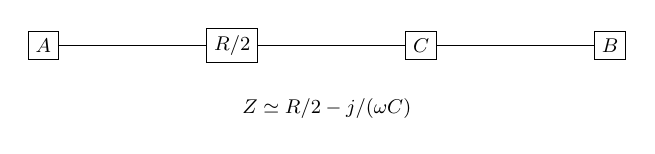
\begin{tikzpicture}[scale=.8,transform shape]
\node[draw] (a) at (0,0) {$A$};\node[draw] (r) at (3,0) {$R/2$};\node[draw] (c) at (6,0) {$C$};\node[draw] (b) at (9,0) {$B$};\draw (a)--(r)--(c)--(b);\node at (4.5,-1) {$Z\simeq R/2-j/(\omega C)$};
\end{tikzpicture}
\figcaption{变图电试4.4V2\quad 低频主导的串联等效形式}
\end{minipage}\end{center}

\Needspace{20\baselineskip}
\item 求高频时的电阻实部和电抗主导项，并解释等效电感。
\textbf{解：}变图电试4.4V3对$x\to\infty$展开，$\Re Z\to R/4$，$-Rx/[4(1+x^2)]\simeq-1/(4\omega C)$，所以$\Im Z\simeq\omega L/2-5/(4\omega C)$。两电感电流各为$I/2$，无功之和为$2\omega L|I/2|^2$，对应端口电感$L/2$。此时$I_1/I\to1/4$、$I_2/I\to-1/4$，四电阻热功率为$4R|I/4|^2$，给实部$R/4$。
\begin{center}\begin{minipage}{.98\linewidth}\centering
\begin{tikzpicture}[scale=.8,transform shape]
\node[draw] (a) at (0,0) {$A$};\node[draw] (r) at (3,0) {$R/4$};\node[draw] (l) at (6,0) {$L/2$};\node[draw] (b) at (9,0) {$B$};\draw (a)--(r)--(l)--(b);\node at (4.5,-1) {高频主导项，电抗还含$-5/(4\omega C)$};
\end{tikzpicture}
\figcaption{变图电试4.4V3\quad 高频的等效电阻与电感，保留首项电容修正}
\end{minipage}\end{center}

\Needspace{20\baselineskip}
\item 特殊频率下端电压有效值为$V$，求有功、无功和视在功率。
\textbf{解：}变图电试4.4V4由$Z=R(3-5j)/8$得$|Z|^2=34R^2/64$，有效电流平方为$64V^2/(34R^2)$。复功率$I^2Z$给$P=12V^2/(17R)$、$Q=-20V^2/(17R)$，视在功率$S=8V^2/(\sqrt{34}R)$。三者满足$P^2+Q^2=S^2$，$Q<0$与容性超前相同；有功功率保持正值，来自四个电阻的耗散。
\begin{center}\begin{minipage}{.98\linewidth}\centering
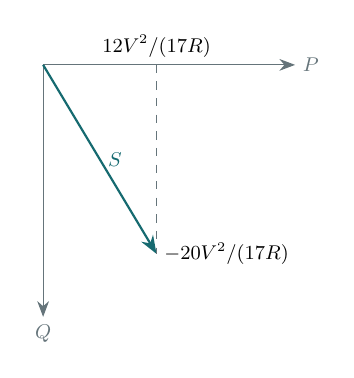
\begin{tikzpicture}[scale=.8,transform shape]
\draw[axis] (0,0)--(4,0) node[right] {$P$};\draw[axis] (0,0)--(0,-4) node[below] {$Q$};\draw[motion] (0,0)--(1.8,-3) node[midway,right] {$S$};\draw[guide] (1.8,0)--(1.8,-3);\node[above] at (1.8,0) {$12V^2/(17R)$};\node[right] at (1.8,-3) {$-20V^2/(17R)$};
\end{tikzpicture}
\figcaption{变图电试4.4V4\quad 特殊频率的有功与容性无功组成的功率三角形}
\end{minipage}\end{center}

\Needspace{20\baselineskip}
\item 证明一般频率下四个电阻的总耗散恰给阻抗实部，并讨论改变$L$的影响。
\textbf{解：}变图电试4.4V5记$a=I_1/I=(R/2+Z_c)/[2(R+Z_c)]$、$b=I_2/I=-R/[4(R+Z_c)]$。以$x=\omega RC$表示，$|a|^2=(x^2+4)/[16(1+x^2)]$、$|b|^2=x^2/[16(1+x^2)]$，故$P/|I|^2=2R(|a|^2+|b|^2)=R(2+x^2)/[4(1+x^2)]=\Re Z$。这些电流比例由$R,C,\omega$决定，固定端口电流时改变$L$保持四电阻耗散相同，只改变端口电抗。
\begin{center}\begin{minipage}{.98\linewidth}\centering
\begin{tikzpicture}[scale=.8,transform shape]
\draw[axis] (0,0)--(10.7,0) node[right] {$x=\omega RC$};
\draw[axis] (0,0)--(0,3.2) node[above] {$P/(R|I|^2)$};\foreach \y/\lab in {0/0,1.35/0.25,2.7/0.5}{\draw[thin] (0,\y)--(-.08,\y) node[left] {$\lab$};}
\node[above] at (5,3.5) {实线两外电阻，虚线两内电阻；总和给$\Re Z/R$};
\draw[traj] plot coordinates {(0.125000000,2.694950125) (0.207291667,2.686172838) (0.289583333,2.673189569) (0.371875000,2.656163658) (0.454166667,2.635304506) (0.536458333,2.610861316) (0.618750000,2.583115971) (0.701041667,2.552375389) (0.783333333,2.518963738) (0.865625000,2.483214820) (0.947916667,2.445464929) (1.030208333,2.406046385) (1.112500000,2.365281922) (1.194791667,2.323480011) (1.277083333,2.280931151) (1.359375000,2.237905122) (1.441666667,2.194649126) (1.523958333,2.151386736) (1.606250000,2.108317555) (1.688541667,2.065617457) (1.770833333,2.023439306) (1.853125000,1.981914039) (1.935416667,1.941152014) (2.017708333,1.901244535) (2.100000000,1.862265478) (2.182291667,1.824272960) (2.264583333,1.787310986) (2.346875000,1.751411066) (2.429166667,1.716593738) (2.511458333,1.682870010) (2.593750000,1.650242682) (2.676041667,1.618707568) (2.758333333,1.588254594) (2.840625000,1.558868781) (2.922916667,1.530531129) (3.005208333,1.503219389) (3.087500000,1.476908741) (3.169791667,1.451572388) (3.252083333,1.427182063) (3.334375000,1.403708471) (3.416666667,1.381121658) (3.498958333,1.359391330) (3.581250000,1.338487116) (3.663541667,1.318378789) (3.745833333,1.299036446) (3.828125000,1.280430657) (3.910416667,1.262532583) (3.992708333,1.245314067) (4.075000000,1.228747710) (4.157291667,1.212806918) (4.239583333,1.197465946) (4.321875000,1.182699920) (4.404166667,1.168484849) (4.486458333,1.154797636) (4.568750000,1.141616069) (4.651041667,1.128918815) (4.733333333,1.116685409) (4.815625000,1.104896231) (4.897916667,1.093532492) (4.980208333,1.082576207) (5.062500000,1.072010170) (5.144791667,1.061817932) (5.227083333,1.051983770) (5.309375000,1.042492665) (5.391666667,1.033330269) (5.473958333,1.024482884) (5.556250000,1.015937431) (5.638541667,1.007681423) (5.720833333,0.999702946) (5.803125000,0.991990624) (5.885416667,0.984533603) (5.967708333,0.977321523) (6.050000000,0.970344496) (6.132291667,0.963593084) (6.214583333,0.957058279) (6.296875000,0.950731481) (6.379166667,0.944604480) (6.461458333,0.938669437) (6.543750000,0.932918865) (6.626041667,0.927345615) (6.708333333,0.921942854) (6.790625000,0.916704058) (6.872916667,0.911622991) (6.955208333,0.906693691) (7.037500000,0.901910460) (7.119791667,0.897267850) (7.202083333,0.892760651) (7.284375000,0.888383878) (7.366666667,0.884132762) (7.448958333,0.880002738) (7.531250000,0.875989439) (7.613541667,0.872088680) (7.695833333,0.868296458) (7.778125000,0.864608933) (7.860416667,0.861022430) (7.942708333,0.857533426) (8.025000000,0.854138543) (8.107291667,0.850834542) (8.189583333,0.847618319) (8.271875000,0.844486893) (8.354166667,0.841437406) (8.436458333,0.838467115) (8.518750000,0.835573386) (8.601041667,0.832753689) (8.683333333,0.830005596) (8.765625000,0.827326774) (8.847916667,0.824714979) (8.930208333,0.822168058) (9.012500000,0.819683937) (9.094791667,0.817260625) (9.177083333,0.814896205) (9.259375000,0.812588834) (9.341666667,0.810336738) (9.423958333,0.808138209) (9.506250000,0.805991602) (9.588541667,0.803895336) (9.670833333,0.801847886) (9.753125000,0.799847782) (9.835416667,0.797893608) (9.917708333,0.795984002) (10.000000000,0.794117647)};
\draw[dashed,thick,color=warm] plot coordinates {(0.125000000,0.001683292) (0.207291667,0.004609054) (0.289583333,0.008936810) (0.371875000,0.014612114) (0.454166667,0.021565165) (0.536458333,0.029712895) (0.618750000,0.038961343) (0.701041667,0.049208204) (0.783333333,0.060345421) (0.865625000,0.072261727) (0.947916667,0.084845024) (1.030208333,0.097984538) (1.112500000,0.111572693) (1.194791667,0.125506663) (1.277083333,0.139689616) (1.359375000,0.154031626) (1.441666667,0.168450291) (1.523958333,0.182871088) (1.606250000,0.197227482) (1.688541667,0.211460848) (1.770833333,0.225520231) (1.853125000,0.239361987) (1.935416667,0.252949329) (2.017708333,0.266251822) (2.100000000,0.279244841) (2.182291667,0.291909013) (2.264583333,0.304229671) (2.346875000,0.316196311) (2.429166667,0.327802087) (2.511458333,0.339043330) (2.593750000,0.349919106) (2.676041667,0.360430811) (2.758333333,0.370581802) (2.840625000,0.380377073) (2.922916667,0.389822957) (3.005208333,0.398926870) (3.087500000,0.407697086) (3.169791667,0.416142537) (3.252083333,0.424272646) (3.334375000,0.432097176) (3.416666667,0.439626114) (3.498958333,0.446869557) (3.581250000,0.453837628) (3.663541667,0.460540404) (3.745833333,0.466987851) (3.828125000,0.473189781) (3.910416667,0.479155806) (3.992708333,0.484895311) (4.075000000,0.490417430) (4.157291667,0.495731027) (4.239583333,0.500844685) (4.321875000,0.505766693) (4.404166667,0.510505050) (4.486458333,0.515067455) (4.568750000,0.519461310) (4.651041667,0.523693728) (4.733333333,0.527771530) (4.815625000,0.531701256) (4.897916667,0.535489169) (4.980208333,0.539141264) (5.062500000,0.542663277) (5.144791667,0.546060689) (5.227083333,0.549338743) (5.309375000,0.552502445) (5.391666667,0.555556577) (5.473958333,0.558505705) (5.556250000,0.561354190) (5.638541667,0.564106192) (5.720833333,0.566765685) (5.803125000,0.569336459) (5.885416667,0.571822132) (5.967708333,0.574226159) (6.050000000,0.576551835) (6.132291667,0.578802305) (6.214583333,0.580980574) (6.296875000,0.583089506) (6.379166667,0.585131840) (6.461458333,0.587110188) (6.543750000,0.589027045) (6.626041667,0.590884795) (6.708333333,0.592685715) (6.790625000,0.594431981) (6.872916667,0.596125670) (6.955208333,0.597768770) (7.037500000,0.599363180) (7.119791667,0.600910717) (7.202083333,0.602413116) (7.284375000,0.603872041) (7.366666667,0.605289079) (7.448958333,0.606665754) (7.531250000,0.608003520) (7.613541667,0.609303773) (7.695833333,0.610567847) (7.778125000,0.611797022) (7.860416667,0.612992523) (7.942708333,0.614155525) (8.025000000,0.615287152) (8.107291667,0.616388486) (8.189583333,0.617460560) (8.271875000,0.618504369) (8.354166667,0.619520865) (8.436458333,0.620510962) (8.518750000,0.621475538) (8.601041667,0.622415437) (8.683333333,0.623331468) (8.765625000,0.624224409) (8.847916667,0.625095007) (8.930208333,0.625943981) (9.012500000,0.626772021) (9.094791667,0.627579792) (9.177083333,0.628367932) (9.259375000,0.629137055) (9.341666667,0.629887754) (9.423958333,0.630620597) (9.506250000,0.631336133) (9.588541667,0.632034888) (9.670833333,0.632717371) (9.753125000,0.633384073) (9.835416667,0.634035464) (9.917708333,0.634671999) (10.000000000,0.635294118)};
\node[below] at (0,-.12) {$0$极限};
\node[below] at (2.5,-.12) {$1$};
\node[below] at (10,-.12) {$4$};
\end{tikzpicture}
\figcaption{变图电试4.4V5\quad 实线两外电阻，虚线两内电阻；总和给$\Re Z/R$}
\end{minipage}\end{center}

\Needspace{20\baselineskip}
\item 固定$R,L,\omega$而调$C$，求端口同相条件，并说明正电容解的唯一性。
\textbf{解：}变图电试4.4V6令$x=\omega RC>0$、$\lambda=\omega L/R>0$，零电抗条件为$\lambda/2=F(x)=1/x+x/[4(1+x^2)]$，也即$2\lambda x^3-5x^2+2\lambda x-4=0$。$F'(x)=-[4+7x^2+5x^4]/[4x^2(1+x^2)^2]<0$，且$F(0^+)=\infty,F(\infty)=0$，所以每个正$\lambda$对应唯一正$x$。求该根后$C=x/(\omega R)$，其他代数根按正实电容条件选去。
\begin{center}\begin{minipage}{.98\linewidth}\centering
\begin{tikzpicture}[scale=.8,transform shape]
\draw[axis] (0,0)--(10.7,0) node[right] {$x=\omega RC$};
\draw[axis] (0,0)--(0,3.2) node[above] {$F(x)$};\foreach \y/\lab in {0/0,1.1/1,2.2/2}{\draw[thin] (0,\y)--(-.08,\y) node[left] {$\lab$};}
\node[above] at (5,3.5) {严格递减函数与$\lambda/2$相交一次};
\draw[traj] plot coordinates {(1.000000000,2.844827586) (1.075000000,2.657936986) (1.150000000,2.495711743) (1.225000000,2.353558551) (1.300000000,2.227947588) (1.375000000,2.116122841) (1.450000000,2.015902218) (1.525000000,1.925536541) (1.600000000,1.843608116) (1.675000000,1.768956481) (1.750000000,1.700623202) (1.825000000,1.637810239) (1.900000000,1.579848137) (1.975000000,1.526171457) (2.050000000,1.476299578) (2.125000000,1.429821566) (2.200000000,1.386384130) (2.275000000,1.345681970) (2.350000000,1.307449971) (2.425000000,1.271456859) (2.500000000,1.237500000) (2.575000000,1.205401118) (2.650000000,1.175002754) (2.725000000,1.146165309) (2.800000000,1.118764575) (2.875000000,1.092689662) (2.950000000,1.067841243) (3.025000000,1.044130071) (3.100000000,1.021475715) (3.175000000,0.999805478) (3.250000000,0.979053474) (3.325000000,0.959159836) (3.400000000,0.940070020) (3.475000000,0.921734220) (3.550000000,0.904106845) (3.625000000,0.887146072) (3.700000000,0.870813454) (3.775000000,0.855073571) (3.850000000,0.839893734) (3.925000000,0.825243713) (4.000000000,0.811095506) (4.075000000,0.797423125) (4.150000000,0.784202418) (4.225000000,0.771410901) (4.300000000,0.759027608) (4.375000000,0.747032967) (4.450000000,0.735408677) (4.525000000,0.724137604) (4.600000000,0.713203686) (4.675000000,0.702591851) (4.750000000,0.692287932) (4.825000000,0.682278606) (4.900000000,0.672551324) (4.975000000,0.663094256) (5.050000000,0.653896240) (5.125000000,0.644946731) (5.200000000,0.636235760) (5.275000000,0.627753896) (5.350000000,0.619492202) (5.425000000,0.611442212) (5.500000000,0.603595890) (5.575000000,0.595945611) (5.650000000,0.588484129) (5.725000000,0.581204552) (5.800000000,0.574100328) (5.875000000,0.567165214) (5.950000000,0.560393265) (6.025000000,0.553778813) (6.100000000,0.547316451) (6.175000000,0.541001018) (6.250000000,0.534827586) (6.325000000,0.528791445) (6.400000000,0.522888093) (6.475000000,0.517113222) (6.550000000,0.511462709) (6.625000000,0.505932607) (6.700000000,0.500519134) (6.775000000,0.495218665) (6.850000000,0.490027723) (6.925000000,0.484942973) (7.000000000,0.479961215) (7.075000000,0.475079375) (7.150000000,0.470294499) (7.225000000,0.465603751) (7.300000000,0.461004401) (7.375000000,0.456493827) (7.450000000,0.452069503) (7.525000000,0.447728999) (7.600000000,0.443469976) (7.675000000,0.439290179) (7.750000000,0.435187437) (7.825000000,0.431159657) (7.900000000,0.427204820) (7.975000000,0.423320978) (8.050000000,0.419506255) (8.125000000,0.415758836) (8.200000000,0.412076971) (8.275000000,0.408458969) (8.350000000,0.404903198) (8.425000000,0.401408079) (8.500000000,0.397972087) (8.575000000,0.394593746) (8.650000000,0.391271630) (8.725000000,0.388004359) (8.800000000,0.384790596) (8.875000000,0.381629050) (8.950000000,0.378518469) (9.025000000,0.375457639) (9.100000000,0.372445388) (9.175000000,0.369480577) (9.250000000,0.366562103) (9.325000000,0.363688898) (9.400000000,0.360859924) (9.475000000,0.358074177) (9.550000000,0.355330681) (9.625000000,0.352628490) (9.700000000,0.349966685) (9.775000000,0.347344376) (9.850000000,0.344760695) (9.925000000,0.342214803) (10.000000000,0.339705882)};
\node[below] at (1,-.12) {$.4$};
\node[below] at (2.5,-.12) {$1$};
\node[below] at (10,-.12) {$4$};
\draw[guide] (1,1.1)--(10,1.1) node[right] {$\lambda/2=1$};
\end{tikzpicture}
\figcaption{变图电试4.4V6\quad 示例取$\lambda=2$，严格递减的$F(x)$与水平线相交一次。}
\end{minipage}\end{center}

\Needspace{20\baselineskip}
\item 元件满足$\omega_0L=1/(\omega_0C)=R$，保持元件不变而改变频率，求端口由容性变感性的频率。
\textbf{解：}变图电试4.4V7令$z=\omega/\omega_0$，则$\Im Z/R=z/2-1/z-z/[4(1+z^2)]$。通分后符号由$2z^4-3z^2-4$决定，置零得$z^2=(3+\sqrt{41})/4$，所以$\omega_r=\omega_0\sqrt{(3+\sqrt{41})/4}$。其下电抗为负、电流超前，其上电抗为正、电流滞后；实部始终为正，在$\omega_r$处功率因数达到1。
\begin{center}\begin{minipage}{.98\linewidth}\centering
\begin{tikzpicture}[scale=.8,transform shape]
\draw[axis] (0,0)--(10.7,0) node[right] {$\omega/\omega_0$};
\draw[axis] (0,0)--(0,3.2) node[above] {$Z/R$};\foreach \y/\lab in {0.81/-1,2.61/1}{\draw[thin] (0,\y)--(-.08,\y) node[left] {$\lab$};}
\node[above] at (5,3.5) {实线电阻，虚线电抗；元件在$\omega_0$满足题设条件};
\draw[traj] plot coordinates {(1.666666667,2.115000000) (1.736111111,2.111988733) (1.805555556,2.108959732) (1.875000000,2.105919881) (1.944444444,2.102875648) (2.013888889,2.099833068) (2.083333333,2.096797753) (2.152777778,2.093774885) (2.222222222,2.090769231) (2.291666667,2.087785146) (2.361111111,2.084826590) (2.430555556,2.081897138) (2.500000000,2.079000000) (2.569444444,2.076138034) (2.638888889,2.073313767) (2.708333333,2.070529412) (2.777777778,2.067786885) (2.847222222,2.065087829) (2.916666667,2.062433628) (2.986111111,2.059825427) (3.055555556,2.057264151) (3.125000000,2.054750520) (3.194444444,2.052285068) (3.263888889,2.049868159) (3.333333333,2.047500000) (3.402777778,2.045180659) (3.472222222,2.042910075) (3.541666667,2.040688073) (3.611111111,2.038514377) (3.680555556,2.036388617) (3.750000000,2.034310345) (3.819444444,2.032279039) (3.888888889,2.030294118) (3.958333333,2.028354943) (4.027777778,2.026460833) (4.097222222,2.024611063) (4.166666667,2.022804878) (4.236111111,2.021041494) (4.305555556,2.019320104) (4.375000000,2.017639885) (4.444444444,2.016000000) (4.513888889,2.014399602) (4.583333333,2.012837838) (4.652777778,2.011313852) (4.722222222,2.009826790) (4.791666667,2.008375796) (4.861111111,2.006960022) (4.930555556,2.005578625) (5.000000000,2.004230769) (5.069444444,2.002915630) (5.138888889,2.001632391) (5.208333333,2.000380250) (5.277777778,1.999158416) (5.347222222,1.997966112) (5.416666667,1.996802575) (5.486111111,1.995667057) (5.555555556,1.994558824) (5.625000000,1.993477157) (5.694444444,1.992421356) (5.763888889,1.991390732) (5.833333333,1.990384615) (5.902777778,1.989402351) (5.972222222,1.988443299) (6.041666667,1.987506837) (6.111111111,1.986592357) (6.180555556,1.985699267) (6.250000000,1.984826990) (6.319444444,1.983974965) (6.388888889,1.983142645) (6.458333333,1.982329499) (6.527777778,1.981535009) (6.597222222,1.980758672) (6.666666667,1.980000000) (6.736111111,1.979258516) (6.805555556,1.978533759) (6.875000000,1.977825279) (6.944444444,1.977132640) (7.013888889,1.976455418) (7.083333333,1.975793201) (7.152777778,1.975145590) (7.222222222,1.974512195) (7.291666667,1.973892640) (7.361111111,1.973286558) (7.430555556,1.972693594) (7.500000000,1.972113402) (7.569444444,1.971545647) (7.638888889,1.970990003) (7.708333333,1.970446154) (7.777777778,1.969913793) (7.847222222,1.969392623) (7.916666667,1.968882353) (7.986111111,1.968382703) (8.055555556,1.967893401) (8.125000000,1.967414181) (8.194444444,1.966944787) (8.263888889,1.966484968) (8.333333333,1.966034483) (8.402777778,1.965593095) (8.472222222,1.965160577) (8.541666667,1.964736706) (8.611111111,1.964321267) (8.680555556,1.963914050) (8.750000000,1.963514851) (8.819444444,1.963123474) (8.888888889,1.962739726) (8.958333333,1.962363420) (9.027777778,1.961994376) (9.097222222,1.961632417) (9.166666667,1.961277372) (9.236111111,1.960929075) (9.305555556,1.960587364) (9.375000000,1.960252082) (9.444444444,1.959923077) (9.513888889,1.959600199) (9.583333333,1.959283305) (9.652777778,1.958972254) (9.722222222,1.958666910) (9.791666667,1.958367140) (9.861111111,1.958072815) (9.930555556,1.957783809) (10.000000000,1.957500000)};
\draw[dashed,thick,color=warm] plot coordinates {(1.666666667,0.045000000) (1.736111111,0.124193368) (1.805555556,0.197983351) (1.875000000,0.266982567) (1.944444444,0.331715396) (2.013888889,0.392633182) (2.083333333,0.450126404) (2.152777778,0.504534500) (2.222222222,0.556153846) (2.291666667,0.605244303) (2.361111111,0.652034597) (2.430555556,0.696726789) (2.500000000,0.739500000) (2.569444444,0.780513531) (2.638888889,0.819909496) (2.708333333,0.857815045) (2.777777778,0.894344262) (2.847222222,0.929599776) (2.916666667,0.963674147) (2.986111111,0.996651058) (3.055555556,1.028606346) (3.125000000,1.059608888) (3.194444444,1.089721375) (3.263888889,1.119000992) (3.333333333,1.147500000) (3.402777778,1.175266258) (3.472222222,1.202343672) (3.541666667,1.228772598) (3.611111111,1.254590194) (3.680555556,1.279830729) (3.750000000,1.304525862) (3.819444444,1.328704889) (3.888888889,1.352394958) (3.958333333,1.375621268) (4.027777778,1.398407241) (4.097222222,1.420774678) (4.166666667,1.442743902) (4.236111111,1.464333880) (4.305555556,1.485562339) (4.375000000,1.506445865) (4.444444444,1.527000000) (4.513888889,1.547239321) (4.583333333,1.567177518) (4.652777778,1.586827461) (4.722222222,1.606201263) (4.791666667,1.625310336) (4.861111111,1.644165444) (4.930555556,1.662776746) (5.000000000,1.681153846) (5.069444444,1.699305825) (5.138888889,1.717241280) (5.208333333,1.734968360) (5.277777778,1.752494789) (5.347222222,1.769827901) (5.416666667,1.786974662) (5.486111111,1.803941693) (5.555555556,1.820735294) (5.625000000,1.837361464) (5.694444444,1.853825916) (5.763888889,1.870134098) (5.833333333,1.886291209) (5.902777778,1.902302210) (5.972222222,1.918171841) (6.041666667,1.933904634) (6.111111111,1.949504922) (6.180555556,1.964976852) (6.250000000,1.980324394) (6.319444444,1.995551355) (6.388888889,2.010661380) (6.458333333,2.025657967) (6.527777778,2.040544473) (6.597222222,2.055324119) (6.666666667,2.070000000) (6.736111111,2.084575090) (6.805555556,2.099052249) (6.875000000,2.113434226) (6.944444444,2.127723667) (7.013888889,2.141923119) (7.083333333,2.156035036) (7.152777778,2.170061780) (7.222222222,2.184005629) (7.291666667,2.197868778) (7.361111111,2.211653347) (7.430555556,2.225361379) (7.500000000,2.238994845) (7.569444444,2.252555652) (7.638888889,2.266045638) (7.708333333,2.279466580) (7.777777778,2.292820197) (7.847222222,2.306108149) (7.916666667,2.319332043) (7.986111111,2.332493433) (8.055555556,2.345593821) (8.125000000,2.358634664) (8.194444444,2.371617371) (8.263888889,2.384543306) (8.333333333,2.397413793) (8.402777778,2.410230112) (8.472222222,2.422993506) (8.541666667,2.435705178) (8.611111111,2.448366297) (8.680555556,2.460977995) (8.750000000,2.473541372) (8.819444444,2.486057494) (8.888888889,2.498527397) (8.958333333,2.510952087) (9.027777778,2.523332539) (9.097222222,2.535669702) (9.166666667,2.547964499) (9.236111111,2.560217824) (9.305555556,2.572430548) (9.375000000,2.584603518) (9.444444444,2.596737557) (9.513888889,2.608833464) (9.583333333,2.620892019) (9.652777778,2.632913980) (9.722222222,2.644900083) (9.791666667,2.656851048) (9.861111111,2.668767571) (9.930555556,2.680650334) (10.000000000,2.692500000)};
\node[below] at (1.6666666666666667,-.12) {$1/2$};
\node[below] at (3.3333333333333335,-.12) {$1$};
\node[below] at (10,-.12) {$3$};
\draw[dotted] (0,1.71)--(10,1.71);\node[left] at (0,1.71) {$0$};
\end{tikzpicture}
\figcaption{变图电试4.4V7\quad 实线电阻，虚线电抗；元件在$\omega_0$满足题设条件}
\end{minipage}\end{center}

\Needspace{20\baselineskip}
\item 固定$R,C,\omega$和端电压有效值$V$，改变$L$，求有功功率最大值及其条件。
\textbf{解：}变图电试4.4V8记$A=\Re Z>0$、$B=1/(\omega C)+Rx/[4(1+x^2)]$，则$Z=A+j(\omega L/2-B)$。有功功率$P=V^2A/[A^2+(\omega L/2-B)^2]$，分母在$L=2B/\omega$时最小，故$P_{\max}=V^2/A$。这是同相条件，端电流幅值也在此时最大。若$x=1$，$A=3R/8$、$B=9R/8$，所需$\omega L/R=9/4$，最大功率$8V^2/(3R)$。固定端电压下调$L$改变总电流，固定端电流下的耗散则按上一变式保持相同。
\begin{center}\begin{minipage}{.98\linewidth}\centering
\begin{tikzpicture}[scale=.8,transform shape]
\draw[axis] (0,0)--(10.7,0) node[right] {$\lambda=\omega L/R$};
\draw[axis] (0,0)--(0,3.2) node[above] {$PR/V^2$};\foreach \y/\lab in {0/0,1/1,2/2,3/3}{\draw[thin] (0,\y)--(-.08,\y) node[left] {$\lab$};}
\node[above] at (5,3.5) {固定电压下调L，功率在零电抗处最大};
\draw[traj] plot coordinates {(0.000000000,0.266666667) (0.083333333,0.275774019) (0.166666667,0.285336856) (0.250000000,0.295384615) (0.333333333,0.305949008) (0.416666667,0.317064220) (0.500000000,0.328767123) (0.583333333,0.341097513) (0.666666667,0.354098361) (0.750000000,0.367816092) (0.833333333,0.382300885) (0.916666667,0.397606995) (1.000000000,0.413793103) (1.083333333,0.430922693) (1.166666667,0.449064449) (1.250000000,0.468292683) (1.333333333,0.488687783) (1.416666667,0.510336680) (1.500000000,0.533333333) (1.583333333,0.557779212) (1.666666667,0.583783784) (1.750000000,0.611464968) (1.833333333,0.640949555) (1.916666667,0.672373541) (2.000000000,0.705882353) (2.083333333,0.741630901) (2.166666667,0.779783394) (2.250000000,0.820512821) (2.333333333,0.864000000) (2.416666667,0.910432034) (2.500000000,0.960000000) (2.583333333,1.012895662) (2.666666667,1.069306931) (2.750000000,1.129411765) (2.833333333,1.193370166) (2.916666667,1.261313869) (3.000000000,1.333333333) (3.083333333,1.409461664) (3.166666667,1.489655172) (3.250000000,1.573770492) (3.333333333,1.661538462) (3.416666667,1.752535497) (3.500000000,1.846153846) (3.583333333,1.941573034) (3.666666667,2.037735849) (3.750000000,2.133333333) (3.833333333,2.226804124) (3.916666667,2.316353887) (4.000000000,2.400000000) (4.083333333,2.475644699) (4.166666667,2.541176471) (4.250000000,2.594594595) (4.333333333,2.634146341) (4.416666667,2.658461538) (4.500000000,2.666666667) (4.583333333,2.658461538) (4.666666667,2.634146341) (4.750000000,2.594594595) (4.833333333,2.541176471) (4.916666667,2.475644699) (5.000000000,2.400000000) (5.083333333,2.316353887) (5.166666667,2.226804124) (5.250000000,2.133333333) (5.333333333,2.037735849) (5.416666667,1.941573034) (5.500000000,1.846153846) (5.583333333,1.752535497) (5.666666667,1.661538462) (5.750000000,1.573770492) (5.833333333,1.489655172) (5.916666667,1.409461664) (6.000000000,1.333333333) (6.083333333,1.261313869) (6.166666667,1.193370166) (6.250000000,1.129411765) (6.333333333,1.069306931) (6.416666667,1.012895662) (6.500000000,0.960000000) (6.583333333,0.910432034) (6.666666667,0.864000000) (6.750000000,0.820512821) (6.833333333,0.779783394) (6.916666667,0.741630901) (7.000000000,0.705882353) (7.083333333,0.672373541) (7.166666667,0.640949555) (7.250000000,0.611464968) (7.333333333,0.583783784) (7.416666667,0.557779212) (7.500000000,0.533333333) (7.583333333,0.510336680) (7.666666667,0.488687783) (7.750000000,0.468292683) (7.833333333,0.449064449) (7.916666667,0.430922693) (8.000000000,0.413793103) (8.083333333,0.397606995) (8.166666667,0.382300885) (8.250000000,0.367816092) (8.333333333,0.354098361) (8.416666667,0.341097513) (8.500000000,0.328767123) (8.583333333,0.317064220) (8.666666667,0.305949008) (8.750000000,0.295384615) (8.833333333,0.285336856) (8.916666667,0.275774019) (9.000000000,0.266666667) (9.083333333,0.257987459) (9.166666667,0.249710983) (9.250000000,0.241813602) (9.333333333,0.234273319) (9.416666667,0.227069645) (9.500000000,0.220183486) (9.583333333,0.213597033) (9.666666667,0.207293666) (9.750000000,0.201257862) (9.833333333,0.195475113) (9.916666667,0.189931853) (10.000000000,0.184615385)};
\node[below] at (0,-.12) {$0$};
\node[below] at (4.5,-.12) {$9/4$};
\node[below] at (10,-.12) {$5$};
\end{tikzpicture}
\figcaption{变图电试4.4V8\quad 固定电压下调L，功率在零电抗处最大}
\end{minipage}\end{center}
\end{enumerate}

\Needspace{13\baselineskip}

\pdfbookmark[2]{第 5 题 导体屏蔽暂态与单频等效电容}{q5}

\section*{第 5 题\quad 导体屏蔽暂态与单频等效电容}\label{q:5}


长$l$、截面积$S$的导体，在一维平行面近似下置于沿轴线的外加电场中。$t<0$时无电场且无表面电荷；$t=0$起外加电场为
$E_{\rm ext}(t)=E_0\cos\omega t$。导体电导率为$\sigma=\alpha\varepsilon_0\omega$，$\alpha>0$；在本题给定频率，$\sigma$为实常量。忽略边缘效应、传播延迟及载流子惯性。
\begin{enumerate}
\item 求导体中的传导电流密度$j(t)$，并给出表面电荷随时间的变化。
\item 暂态消失后，以外加电势降$u_{\rm ext}(t)=lE_{\rm ext}(t)$为输入、传导电流$i(t)=Sj(t)$为输出，求单频并联电阻$R_p$与电容$C_p$的等效值。
\item 在普通准静态、无色散且相对介电常数$\varepsilon_r\ge1$的介质模型内，能否用相同$l,S$的一个填充介质电容实现该$C_p$？说明该比较的适用范围，并给出可实现端口等效的电阻、电容网络。
\end{enumerate}
导体内部总电场包含表面电荷的屏蔽场；这里输出专指传导电流。


\begin{center}\begin{minipage}{.98\linewidth}\centering
\begin{tikzpicture}[scale=.9,transform shape]

\fill[muted!8] (0,-1) rectangle (6,1);
\draw[object] (0,-1) rectangle (6,1);
\draw[object] (0,-1.2)--(0,1.2);\draw[object] (6,-1.2)--(6,1.2);
\foreach \y in {-.65,0,.65}{\node[left] at (0,\y) {$-$};\node[right] at (6,\y) {$+$};}
\node[above] at (0,1.2) {$-s$};\node[above] at (6,1.2) {$s$};
\draw[motion] (1,2.2)--(5,2.2) node[midway,above] {$E_{\rm ext}=E_0\cos\omega t$};
\draw[force] (4,.1)--(2,.1) node[midway,above] {$E_{\rm ind}=-s/\varepsilon_0$};
\draw[axis,<->] (0,-1.8)--(6,-1.8) node[midway,below] {$l$};
\node at (3,-3) {一维平行面近似；截面积$S$};

\end{tikzpicture}
\figcaption{图电试4.5\quad 场箭头按外场与右端正电荷均为正时示意，实际符号随时间变化。}
\end{minipage}\end{center}

\Needspace{8\baselineskip}

\pdfbookmark[3]{题型定位}{q5-h0}

\subsection*{题型定位}

表面电荷积累的屏蔽暂态及给定频率的并联等效。右表面电荷变化率给传导电流，屏蔽场改变导体内部场，由欧姆定律建立一阶方程。时域解确定初态与指数衰减，稳态相量给外加电势降到传导电流的导纳，再分别讨论网络实现与指定材料模型中的电容实现。

\Needspace{8\baselineskip}

\pdfbookmark[3]{知识点}{q5-h1}

\subsection*{知识点}

平行面电荷产生大小$s/\varepsilon_0$、指向负面的屏蔽场，内部总场由外场与屏蔽场相加。电荷连续性为$j=\dot s$，电导率为固定实常量时得到稳定的一阶线性方程。积分因子给受迫项和齐次项，初始面电荷决定齐次系数。余弦相量中正虚部导纳对应电流超前，电流投影与并联电阻、电容逐项对应。单频并联参数是导纳的等效量，固定串联$R_b,C_0$则直接满足完整时域方程。

\Needspace{8\baselineskip}

\pdfbookmark[3]{物理图像}{q5-h2}

\subsection*{物理图像}

题图和解图电试4.5A统一以外场向右为正，右表面$s$的增加对应向右传导电流，屏蔽场向左。图B将启动电流和周期稳态放在同一相位轴，初始屏蔽尚未形成。图D把稳态电流投影为同相与超前四分之一周期的两部分，图C并列比较指定材料电容、串联网络和单频并联网络，分别对应材料电容公式、完整时域关系和单频导纳。

\Needspace{8\baselineskip}

\pdfbookmark[3]{解题入口}{q5-h3}

\subsection*{解题入口}

先以右表面薄层为控制体写$j=\dot s$，把两个表面电荷产生的屏蔽场代入欧姆定律。求积分时保留下限零与初值，求导后把$t=0^+$的场、电荷和电流放在一起。长期相量采用外加电势降$lE_{\rm ext}$为输入，由投影或导纳求$R_p,C_p$。最后用$q=sS$把屏蔽问题直接写成串联$RC$方程。

\Needspace{8\baselineskip}

\pdfbookmark[3]{标准解法}{q5-h4}

\subsection*{标准解法}


图电试4.5规定向右为正。右端表面电荷面密度记为$s(t)$，左端为$-s(t)$，屏蔽场沿$-x$。内部总场及欧姆定律为
\[
E_{\rm in}=E_{\rm ext}-\frac{s}{\varepsilon_0},\qquad
j=\sigma E_{\rm in}.
\]
\begin{center}\begin{minipage}{.98\linewidth}\centering
\begin{tikzpicture}[scale=.8,transform shape]

\fill[muted!8] (0,-1) rectangle (6,1);
\draw[object] (0,-1) rectangle (6,1);
\draw[object] (0,-1.2)--(0,1.2);\draw[object] (6,-1.2)--(6,1.2);
\foreach \y in {-.65,0,.65}{\node[left] at (0,\y) {$-$};\node[right] at (6,\y) {$+$};}
\node[above] at (0,1.2) {$-s$};\node[above] at (6,1.2) {$s$};
\draw[motion] (1,2.2)--(5,2.2) node[midway,above] {$E_{\rm ext}=E_0\cos\omega t$};
\draw[force] (4,.1)--(2,.1) node[midway,above] {$E_{\rm ind}=-s/\varepsilon_0$};
\draw[axis,<->] (0,-1.8)--(6,-1.8) node[midway,below] {$l$};
\node at (3,-3) {一维平行面近似；截面积$S$};

\draw[motion] (3,-.4)--(5,-.4) node[midway,below] {$j=\dot s$};
\draw[guide] (5.65,-1.4) rectangle (6.35,1.4);
\node[align=left] at (9,0) {右端薄层\\$\dot q=Sj$\\$q=sS$};

\end{tikzpicture}
\figcaption{解图电试4.5A\quad 右表面控制体确定连续性符号，内部总场为两场相加。}
\end{minipage}\end{center}
解图电试4.5A以两端薄层的电荷积累说明连续性：向右的传导电流使右端正电荷增加，所以向右传导电流满足$j=\dot s$。取右表面面积$\Delta S$的薄层，单位时间流入的电量为$j\Delta S$，没有向外传出的传导电流；层内增加的电量为$\dot s\Delta S$，消去面积后给出上述连续性。屏蔽场随$s$增加而增强，从而降低下一时刻内部场和传导电流，反馈方向使自由响应衰减。由此
\[
\dot s+\frac{\sigma}{\varepsilon_0}s
=\sigma E_0\cos\omega t,\qquad s(0)=0.
\]
令$\tau=\varepsilon_0/\sigma$、$\theta=\omega t$，
$\alpha=1/(\omega\tau)$。乘积分因子$e^{t/\tau}$并积分：
\[
\begin{aligned}
s(t)
&=\sigma E_0e^{-t/\tau}\int_0^t e^{u/\tau}\cos\omega u\,du\\
&=\frac{\sigma E_0}{\tau^{-2}+\omega^2}
\left[\tau^{-1}\cos\omega t+\omega\sin\omega t
-\tau^{-1}e^{-t/\tau}\right]\\
&=\boxed{\frac{\alpha\varepsilon_0E_0}{1+\alpha^2}
\left[\sin\theta+\alpha\cos\theta-\alpha e^{-\alpha\theta}\right]}.
\end{aligned}
\]
积分时用到$\int e^{au}\cos\omega u\,\mathrm du=e^{au}(a\cos\omega u+\omega\sin\omega u)/(a^2+\omega^2)$，取$a=1/\tau$，并在上、下限相减。若先写不定积分，齐次系数由$s(0)=0$得$-\alpha^2\varepsilon_0E_0/(1+\alpha^2)$，正好是最后指数项的系数。

求时间导数得到传导电流密度
\[
\boxed{j(t)=\frac{\sigma E_0}{1+\alpha^2}
\left[\cos\theta-\alpha\sin\theta+\alpha^2e^{-\alpha\theta}\right]}.
\]
括号中的三项求导依次给$\omega\cos\theta$、$-\alpha\omega\sin\theta$和$+\alpha^2\omega e^{-\alpha\theta}$；前面的$\alpha\varepsilon_0\omega$即为$\sigma$。初始时$s(0)=0$、$j(0+)=\sigma E_0$：屏蔽电荷尚未积累，内部场等于刚接入的外场。指数项把电流从无屏蔽的初始值接到周期响应。
\begin{center}\begin{minipage}{.98\linewidth}\centering
\begin{tikzpicture}[scale=.8,transform shape]
\draw[axis] (0,0)--(10.7,0) node[right] {$\theta=\omega t$};
\draw[axis] (0,0)--(0,3.2) node[above] {$j/(\sigma E_0)$};\foreach \y/\lab in {0.45/-0.5,1.95/0.5,2.7/1}{\draw[thin] (0,\y)--(-.08,\y) node[left] {$\lab$};}
\node[above] at (5,3.5) {$\alpha=1$：实线完整响应，虚线周期稳态};
\draw[traj] plot coordinates {(0.000000000,2.700000000) (0.062500000,2.625000387) (0.125000000,2.550006125) (0.187500000,2.475030691) (0.250000000,2.400096000) (0.312500000,2.325231934) (0.375000000,2.250475877) (0.437500000,2.175872246) (0.500000000,2.101472023) (0.562500000,2.027332290) (0.625000000,1.953515762) (0.687500000,1.880090328) (0.750000000,1.807128583) (0.812500000,1.734707377) (0.875000000,1.662907353) (0.937500000,1.591812496) (1.000000000,1.521509687) (1.062500000,1.452088255) (1.125000000,1.383639539) (1.187500000,1.316256456) (1.250000000,1.250033072) (1.312500000,1.185064179) (1.375000000,1.121444884) (1.437500000,1.059270203) (1.500000000,0.998634660) (1.562500000,0.939631905) (1.625000000,0.882354327) (1.687500000,0.826892692) (1.750000000,0.773335783) (1.812500000,0.721770050) (1.875000000,0.672279281) (1.937500000,0.624944278) (2.000000000,0.579842544) (2.062500000,0.537047994) (2.125000000,0.496630664) (2.187500000,0.458656456) (2.250000000,0.423186872) (2.312500000,0.390278787) (2.375000000,0.359984224) (2.437500000,0.332350144) (2.500000000,0.307418265) (2.562500000,0.285224883) (2.625000000,0.265800718) (2.687500000,0.249170776) (2.750000000,0.235354228) (2.812500000,0.224364304) (2.875000000,0.216208208) (2.937500000,0.210887049) (3.000000000,0.208395793) (3.062500000,0.208723223) (3.125000000,0.211851929) (3.187500000,0.217758310) (3.250000000,0.226412590) (3.312500000,0.237778857) (3.375000000,0.251815118) (3.437500000,0.268473368) (3.500000000,0.287699679) (3.562500000,0.309434303) (3.625000000,0.333611794) (3.687500000,0.360161142) (3.750000000,0.389005923) (3.812500000,0.420064468) (3.875000000,0.453250042) (3.937500000,0.488471037) (4.000000000,0.525631179) (4.062500000,0.564629750) (4.125000000,0.605361819) (4.187500000,0.647718485) (4.250000000,0.691587135) (4.312500000,0.736851701) (4.375000000,0.783392943) (4.437500000,0.831088726) (4.500000000,0.879814312) (4.562500000,0.929442660) (4.625000000,0.979844727) (4.687500000,1.030889780) (4.750000000,1.082445713) (4.812500000,1.134379361) (4.875000000,1.186556825) (4.937500000,1.238843797) (5.000000000,1.291105885) (5.062500000,1.343208939) (5.125000000,1.395019380) (5.187500000,1.446404521) (5.250000000,1.497232896) (5.312500000,1.547374577) (5.375000000,1.596701493) (5.437500000,1.645087744) (5.500000000,1.692409908) (5.562500000,1.738547344) (5.625000000,1.783382486) (5.687500000,1.826801135) (5.750000000,1.868692734) (5.812500000,1.908950645) (5.875000000,1.947472403) (5.937500000,1.984159978) (6.000000000,2.018920004) (6.062500000,2.051664019) (6.125000000,2.082308674) (6.187500000,2.110775941) (6.250000000,2.136993305) (6.312500000,2.160893942) (6.375000000,2.182416879) (6.437500000,2.201507148) (6.500000000,2.218115919) (6.562500000,2.232200617) (6.625000000,2.243725029) (6.687500000,2.252659391) (6.750000000,2.258980458) (6.812500000,2.262671563) (6.875000000,2.263722653) (6.937500000,2.262130317) (7.000000000,2.257897785) (7.062500000,2.251034927) (7.125000000,2.241558220) (7.187500000,2.229490707) (7.250000000,2.214861938) (7.312500000,2.197707897) (7.375000000,2.178070905) (7.437500000,2.155999519) (7.500000000,2.131548403) (7.562500000,2.104778196) (7.625000000,2.075755358) (7.687500000,2.044551998) (7.750000000,2.011245698) (7.812500000,1.975919317) (7.875000000,1.938660781) (7.937500000,1.899562863) (8.000000000,1.858722953) (8.062500000,1.816242810) (8.125000000,1.772228308) (8.187500000,1.726789170) (8.250000000,1.680038697) (8.312500000,1.632093479) (8.375000000,1.583073105) (8.437500000,1.533099863) (8.500000000,1.482298436) (8.562500000,1.430795586) (8.625000000,1.378719841) (8.687500000,1.326201168) (8.750000000,1.273370653) (8.812500000,1.220360169) (8.875000000,1.167302048) (8.937500000,1.114328750) (9.000000000,1.061572527) (9.062500000,1.009165101) (9.125000000,0.957237327) (9.187500000,0.905918865) (9.250000000,0.855337863) (9.312500000,0.805620630) (9.375000000,0.756891319) (9.437500000,0.709271624) (9.500000000,0.662880466) (9.562500000,0.617833705) (9.625000000,0.574243842) (9.687500000,0.532219740) (9.750000000,0.491866358) (9.812500000,0.453284477) (9.875000000,0.416570457) (9.937500000,0.381815994) (10.000000000,0.349107887)};
\draw[dashed,thick,color=warm] plot coordinates {(0.000000000,1.950000000) (0.062500000,1.911578318) (0.125000000,1.871378061) (0.187500000,1.829499709) (0.250000000,1.786047935) (0.312500000,1.741131347) (0.375000000,1.694862212) (0.437500000,1.647356179) (0.500000000,1.598731989) (0.562500000,1.549111176) (0.625000000,1.498617767) (0.687500000,1.447377970) (0.750000000,1.395519856) (0.812500000,1.343173045) (0.875000000,1.290468375) (0.937500000,1.237537582) (1.000000000,1.184512964) (1.062500000,1.131527056) (1.125000000,1.078712294) (1.187500000,1.026200689) (1.250000000,0.974123491) (1.312500000,0.922610867) (1.375000000,0.871791571) (1.437500000,0.821792625) (1.500000000,0.772739001) (1.562500000,0.724753307) (1.625000000,0.677955482) (1.687500000,0.632462497) (1.750000000,0.588388060) (1.812500000,0.545842334) (1.875000000,0.504931661) (1.937500000,0.465758298) (2.000000000,0.428420156) (2.062500000,0.393010562) (2.125000000,0.359618021) (2.187500000,0.328325998) (2.250000000,0.299212706) (2.312500000,0.272350913) (2.375000000,0.247807759) (2.437500000,0.225644590) (2.500000000,0.205916802) (2.562500000,0.188673705) (2.625000000,0.173958397) (2.687500000,0.161807658) (2.750000000,0.152251859) (2.812500000,0.145314885) (2.875000000,0.141014075) (2.937500000,0.139360178) (3.000000000,0.140357328) (3.062500000,0.144003033) (3.125000000,0.150288180) (3.187500000,0.159197061) (3.250000000,0.170707406) (3.312500000,0.184790447) (3.375000000,0.201410983) (3.437500000,0.220527472) (3.500000000,0.242092132) (3.562500000,0.266051063) (3.625000000,0.292344379) (3.687500000,0.320906362) (3.750000000,0.351665622) (3.812500000,0.384545275) (3.875000000,0.419463140) (3.937500000,0.456331942) (4.000000000,0.495059526) (4.062500000,0.535549094) (4.125000000,0.577699443) (4.187500000,0.621405220) (4.250000000,0.666557182) (4.312500000,0.713042474) (4.375000000,0.760744905) (4.437500000,0.809545246) (4.500000000,0.859321520) (4.562500000,0.909949313) (4.625000000,0.961302082) (4.687500000,1.013251471) (4.750000000,1.065667634) (4.812500000,1.118419558) (4.875000000,1.171375391) (4.937500000,1.224402771) (5.000000000,1.277369156) (5.062500000,1.330142158) (5.125000000,1.382589873) (5.187500000,1.434581209) (5.250000000,1.485986213) (5.312500000,1.536676401) (5.375000000,1.586525074) (5.437500000,1.635407634) (5.500000000,1.683201903) (5.562500000,1.729788418) (5.625000000,1.775050739) (5.687500000,1.818875732) (5.750000000,1.861153858) (5.812500000,1.901779443) (5.875000000,1.940650946) (5.937500000,1.977671206) (6.000000000,2.012747694) (6.062500000,2.045792736) (6.125000000,2.076723737) (6.187500000,2.105463384) (6.250000000,2.131939845) (6.312500000,2.156086942) (6.375000000,2.177844319) (6.437500000,2.197157594) (6.500000000,2.213978495) (6.562500000,2.228264978) (6.625000000,2.239981334) (6.687500000,2.249098278) (6.750000000,2.255593023) (6.812500000,2.259449335) (6.875000000,2.260657575) (6.937500000,2.259214724) (7.000000000,2.255124387) (7.062500000,2.248396789) (7.125000000,2.239048746) (7.187500000,2.227103621) (7.250000000,2.212591272) (7.312500000,2.195547973) (7.375000000,2.176016322) (7.437500000,2.154045138) (7.500000000,2.129689339) (7.562500000,2.103009800) (7.625000000,2.074073207) (7.687500000,2.042951886) (7.750000000,2.009723625) (7.812500000,1.974471476) (7.875000000,1.937283552) (7.937500000,1.898252803) (8.000000000,1.857476785) (8.062500000,1.815057418) (8.125000000,1.771100728) (8.187500000,1.725716584) (8.250000000,1.679018421) (8.312500000,1.631122962) (8.375000000,1.582149921) (8.437500000,1.532221703) (8.500000000,1.481463104) (8.562500000,1.430000994) (8.625000000,1.377964002) (8.687500000,1.325482192) (8.750000000,1.272686742) (8.812500000,1.219709613) (8.875000000,1.166683220) (8.937500000,1.113740101) (9.000000000,1.061012588) (9.062500000,1.008632471) (9.125000000,0.956730673) (9.187500000,0.905436921) (9.250000000,0.854879424) (9.312500000,0.805184548) (9.375000000,0.756476506) (9.437500000,0.708877041) (9.500000000,0.662505128) (9.562500000,0.617476672) (9.625000000,0.573904221) (9.687500000,0.531896684) (9.750000000,0.491559056) (9.812500000,0.452992163) (9.875000000,0.416292399) (9.937500000,0.381551497) (10.000000000,0.348856290)};
\node[below] at (0,-.12) {$0$};
\node[below] at (5,-.12) {$4$};
\node[below] at (10,-.12) {$8$};
\draw[dotted] (0,1.2)--(10,1.2);\node[left] at (0,1.2) {$0$};
\end{tikzpicture}
\figcaption{解图电试4.5B\quad $\alpha=1$：实线完整响应，虚线周期稳态}
\end{minipage}\end{center}
解图电试4.5B显示指数暂态把电流从初始值接到周期稳态。长期响应为
\[
j_{\rm ss}=\frac{\sigma E_0}{1+\alpha^2}
(\cos\theta-\alpha\sin\theta)
=\frac{\sigma E_0}{\sqrt{1+\alpha^2}}
\cos(\theta+\varphi),\qquad
\varphi=\arctan\alpha.
\]
将正、余弦合成时取$\cos\varphi=1/\sqrt{1+\alpha^2}$、$\sin\varphi=\alpha/\sqrt{1+\alpha^2}$，两项都为正，故$0<\varphi<\pi/2$且$\tan\varphi=\alpha$。传导电流超前外加场，但相对于导体内部总场仍由$j=\sigma E_{\rm in}$同相响应；外场决定这里的相位参考，内部总场则进入局部欧姆定律。

第（2）问以$\cos\omega t$对应的复相量为约定，$\widetilde U_{\rm ext}=lE_0$，故
\[
Y_{\rm ext}=\frac{\widetilde I}{\widetilde U_{\rm ext}}
=\frac{\sigma S}{l}\frac{1+\mathrm j\alpha}{1+\alpha^2}.
\]
\begin{center}\begin{minipage}{.98\linewidth}\centering
\begin{tikzpicture}[scale=.8,transform shape]
\draw[axis] (0,0)--(4.2,0) node[right] {$\widetilde U_{\rm ext}$};\draw[motion] (0,0)--(3,0) node[midway,below] {$I_R=I\cos\varphi$};\draw[motion] (0,0)--(0,3) node[above left] {$I_C=I\sin\varphi$};\draw[force] (0,0)--(3,3) node[above right] {$I$};\draw[guide] (0,3)--(3,3)--(3,0);\draw (.7,0) arc(0:45:.7);\node at (1,.45) {$\varphi$};\node at (2,-1) {图取$\alpha=1$；投影式适用于任意$\alpha>0$};
\end{tikzpicture}
\figcaption{解图电试4.5D\quad 稳态电流同相与正交投影决定并联电阻、电容}
\end{minipage}\end{center}
解图电试4.5D中总电流峰值$I_a=\sigma SE_0/\sqrt{1+\alpha^2}$。它沿电压方向的投影$I_R=I_a\cos\varphi=\sigma SE_0/(1+\alpha^2)$，正交投影$I_C=I_a\sin\varphi=\sigma SE_0\alpha/(1+\alpha^2)$。以电压峰值$U_0=lE_0$代入$R_p=U_0/I_R$、$C_p=I_C/(\omega U_0)$，与下列导纳比较得到同一组数值。这些投影是相量幅值分解，两支路瞬时电流分别与电压同相及超前四分之一周期。

与$R_p,C_p$并联导纳$1/R_p+\mathrm j\omega C_p$逐项比较：
\[
\boxed{R_p=\frac{(1+\alpha^2)l}{\sigma S}
=\frac{(1+\alpha^2)l}{\alpha\varepsilon_0\omega S}},
\qquad
\boxed{C_p=\frac{\alpha^2}{1+\alpha^2}\frac{\varepsilon_0S}{l}}.
\]
实部为正、虚部为正，与有耗散且电流超前的结论一致。这组并联元件描述给定单一频率的周期稳态；刚接入时的指数响应由初始电荷进入屏蔽方程。
\begin{center}\begin{minipage}{.98\linewidth}\centering
\begin{tikzpicture}[scale=.8,transform shape]

\node at (1.2,3.3) {同几何单个介质电容};
\draw[object] (0,1.5)--(.9,1.5);\draw[object] (1.5,1.5)--(2.4,1.5);
\draw[object] (.9,.8)--(.9,2.2);\draw[object] (1.5,.8)--(1.5,2.2);
\fill[accent!15] (.95,.85) rectangle (1.45,2.15);
\node at (1.2,.1) {$C_{\rm mat}=\varepsilon_rC_0\ge C_0$};
\begin{scope}[xshift=5cm]
\node at (1.5,3.3) {可实现的串联等效};
\draw[object] (0,1.5)--(.5,1.5);
\draw[object] (.5,1.3) rectangle (1.3,1.7);
\draw[object] (1.3,1.5)--(2,1.5);
\draw[object] (2,1)--(2,2);\draw[object] (2.2,1)--(2.2,2);
\draw[object] (2.2,1.5)--(3,1.5);
\node[above] at (.9,1.7) {$R_b$};\node[above] at (2.1,2) {$C_0$};
\node at (1.5,.1) {$R_bC_0=\varepsilon_0/\sigma$};
\end{scope}
\begin{scope}[yshift=-4.2cm,xshift=3cm]
\node at (1.7,3) {给定频率的并联等效};
\draw[object] (0,0)--(0,1.8)--(1.2,1.8);
\draw[object] (1.2,1.6) rectangle (2.2,2);
\draw[object] (2.2,1.8)--(3.4,1.8)--(3.4,0)--(1.8,0);
\draw[object] (1.8,-.4)--(1.8,.4);\draw[object] (1.6,-.4)--(1.6,.4);
\draw[object] (1.6,0)--(0,0);
\node[above] at (1.7,2) {$R_p$};\node[below] at (1.7,-.4) {$C_p<C_0$};
\draw[object] (0,.9)--(-.7,.9);\draw[object] (3.4,.9)--(4.1,.9);
\end{scope}

\end{tikzpicture}
\figcaption{解图电试4.5C\quad 串联网络具有完整时域等效；固定并联参数只匹配一个频率。}
\end{minipage}\end{center}
第（3）问，解图电试4.5C左侧单个介质电容在题设材料模型下有
\[
C_{\rm mat}=\varepsilon_r C_0\ge C_0,\qquad C_0=\frac{\varepsilon_0S}{l}.
\]
几何固定时，题设介质模型把材料电容的下限设为真空值，改变普通填充介质会使该电容增大。而$0<C_p/C_0=\alpha^2/(1+\alpha^2)<1$，所以在同样几何与该材料模型内，所需数值低于该材料模型中相同几何的最小电容$C_0$。此处$C_p$是整个有耗网络的单频等效参数，$C_p/C_0$由网络电流的投影换算得到，材料相对介电常数则在指定的本构模型内定义。

网络实现则按输入输出关系选元件。电阻描述内部场驱动的焦耳耗散，电容描述屏蔽电荷产生的反向电势降，这两个电压沿同一回路相加，构成串联关系。实际可用导体电阻$R_b=l/(\sigma S)$与真空电容$C_0$串联。其导纳为
\[
Y_{\rm series}=\frac1{R_b+1/(\mathrm j\omega C_0)}
=\frac1{R_b}\frac{1+\mathrm j\alpha}{1+\alpha^2}
=Y_{\rm ext},
\qquad \alpha=\frac1{\omega R_bC_0}.
\]
换算为并联参数也可直接写成
\[
R_p=R_b\left[1+\frac1{\omega^2R_b^2C_0^2}\right],
\qquad
C_p=\frac{C_0}{1+\omega^2R_b^2C_0^2}.
\]
小于$C_0$的数值由串并联换算产生，这个无源串联网络即可实现所需的输入输出关系。

把表面电荷改写为总电荷，令$q=sS$，有
\[
R_b\dot q+\frac q{C_0}=u_{\rm ext}(t),\qquad i=\dot q.
\]
因为$R_b\dot q=l j/\sigma=lE_{\rm in}$，而$q/C_0=l s/\varepsilon_0$，两项相加为外场给定的$lE_{\rm ext}$，这就是串联$RC$的时域方程，且题给$q(0)=0$。因此在$\sigma$固定、上述一维近似有效时，同一组$R_b,C_0$同时再现屏蔽暂态与各频率稳态。相反，$R_p,C_p$随频率改变，每一频率应使用相应的并联值，完整时域响应则由固定串联元件给出。
其中$R_bC_0=\varepsilon_0/\sigma=\tau$，与直接由屏蔽方程求出的衰减时间相同。表面电荷的初值对应串联电容的初始电荷，因此输入波形和初态都能直接放回同一方程。并联换算中的正实部对应电阻热耗散，正虚部对应相对外场的超前电流；各自保持原有物理意义，材料电容的比较则按题设规定的几何和介质模型说明。



\Needspace{8\baselineskip}

\pdfbookmark[3]{关键洞察}{q5-h5}

\subsection*{关键洞察}

电流相对外场的超前由屏蔽电荷的动态形成产生，传导电流对内部总场仍按实电导率同相响应。小于真空几何电容的$C_p$属于有耗网络的单频换算参数；同一输入输出关系可由电阻与真空电容串联实现。与材料公式比较时，几何固定且采用题设的普通无色散介质模型，结论针对这一指定实现方式。

\Needspace{8\baselineskip}

\pdfbookmark[3]{易错点}{q5-h6}

\subsection*{易错点}

正方向由右表面电荷增加确定，$j=\dot s$使自由响应衰减。积分常数保留到代入$s(0)=0$，指数项使$j(0^+)=\sigma E_0$。面电荷求导时只带时间倒数，量纲应为电流除以面积。外加场与内部总场分别出现于端口等效和局部欧姆定律。单频并联值随频率改变，完整暂态则由固定$R_b,C_0$串联模型描述；材料参数按指定介质假设另行比较。

\Needspace{8\baselineskip}

\pdfbookmark[3]{课堂讲解建议}{q5-h7}

\subsection*{课堂讲解建议}

先让学生画右表面的小控制体，由电荷积累决定电流正号，再用两平面电荷的场方向写内部总场。积分后先求零时刻电流，再写长期电流的振幅与相位，说明相位参考使用外场。

把图D电流分解成两投影，一组学生用$U/I_R,I_C/(\omega U)$求并联元件，另一组直接分开复导纳，比较同一组参数。材料问题按题设的几何与介质范围讨论，让学生说明$C_p<C_0$与网络实现的关系：它限定同几何单个材料电容的比较，而串联$R_b,C_0$的导纳仍恰为所求值。接着写串联$RC$的电荷方程，说明这组固定元件怎样再现暂态。最后改变输入的时间变化形式，比较完整串联模型与给定频率并联值各自描述的响应。

\Needspace{8\baselineskip}

\pdfbookmark[3]{变式训练}{q5-h8}

\subsection*{变式训练}

\begin{enumerate}
\Needspace{20\baselineskip}
\item 外场改为恒定$E_0$从零时刻接入，初始面电荷为零，求电荷与电流。
\textbf{解：}变图电试4.5V1中方程为$\dot s+s/\tau=\sigma E_0$。积分因子给$s=\varepsilon_0E_0(1-e^{-t/\tau})$，求导得$j=\sigma E_0e^{-t/\tau}$。初始内部场等于外场，随后屏蔽场逐渐建立，最终$s=\varepsilon_0E_0$使内部总场为零，传导电流随之为零。这与串联$R_b,C_0$接直流后充电完成的状态对应。
\begin{center}\begin{minipage}{.98\linewidth}\centering
\begin{tikzpicture}[scale=.8,transform shape]
\draw[axis] (0,0)--(10.7,0) node[right] {$t/\tau$};
\draw[axis] (0,0)--(0,3.2) node[above] {归一化电荷、电流};\foreach \y/\lab in {0/0,1.4/0.5,2.8/1}{\draw[thin] (0,\y)--(-.08,\y) node[left] {$\lab$};}
\node[above] at (5,3.5) {实线$s/(\varepsilon_0E_0)$，虚线$j/(\sigma E_0)$};
\draw[traj] plot coordinates {(0.000000000,0.000000000) (0.083333333,0.114269520) (0.166666667,0.223875639) (0.250000000,0.329008673) (0.333333333,0.429851170) (0.416666667,0.526578231) (0.500000000,0.619357807) (0.583333333,0.708350999) (0.666666667,0.793712330) (0.750000000,0.875590019) (0.833333333,0.954126235) (0.916666667,1.029457346) (1.000000000,1.101714153) (1.083333333,1.171022120) (1.166666667,1.237501592) (1.250000000,1.301268000) (1.333333333,1.362432067) (1.416666667,1.421099995) (1.500000000,1.477373652) (1.583333333,1.531350752) (1.666666667,1.583125016) (1.750000000,1.632786345) (1.833333333,1.680420968) (1.916666667,1.726111596) (2.000000000,1.769937565) (2.083333333,1.811974972) (2.166666667,1.852296810) (2.250000000,1.890973091) (2.333333333,1.928070973) (2.416666667,1.963654870) (2.500000000,1.997786569) (2.583333333,2.030525334) (2.666666667,2.061928013) (2.750000000,2.092049132) (2.833333333,2.120940991) (2.916666667,2.148653758) (3.000000000,2.175235552) (3.083333333,2.200732528) (3.166666667,2.225188959) (3.250000000,2.248647309) (3.333333333,2.271148312) (3.416666667,2.292731037) (3.500000000,2.313432958) (3.583333333,2.333290023) (3.666666667,2.352336711) (3.750000000,2.370606093) (3.833333333,2.388129891) (3.916666667,2.404938534) (4.000000000,2.421061207) (4.083333333,2.436525905) (4.166666667,2.451359480) (4.250000000,2.465587689) (4.333333333,2.479235237) (4.416666667,2.492325821) (4.500000000,2.504882171) (4.583333333,2.516926090) (4.666666667,2.528478490) (4.750000000,2.539559430) (4.833333333,2.550188151) (4.916666667,2.560383108) (5.000000000,2.570162004) (5.083333333,2.579541817) (5.166666667,2.588538835) (5.250000000,2.597168680) (5.333333333,2.605446337) (5.416666667,2.613386177) (5.500000000,2.621001989) (5.583333333,2.628306995) (5.666666667,2.635313879) (5.750000000,2.642034809) (5.833333333,2.648481455) (5.916666667,2.654665009) (6.000000000,2.660596209) (6.083333333,2.666285353) (6.166666667,2.671742320) (6.250000000,2.676976586) (6.333333333,2.681997238) (6.416666667,2.686812995) (6.500000000,2.691432218) (6.583333333,2.695862928) (6.666666667,2.700112819) (6.750000000,2.704189269) (6.833333333,2.708099357) (6.916666667,2.711849872) (7.000000000,2.715447326) (7.083333333,2.718897967) (7.166666667,2.722207785) (7.250000000,2.725382527) (7.333333333,2.728427707) (7.416666667,2.731348611) (7.500000000,2.734150312) (7.583333333,2.736837673) (7.666666667,2.739415362) (7.750000000,2.741887854) (7.833333333,2.744259442) (7.916666667,2.746534245) (8.000000000,2.748716211) (8.083333333,2.750809130) (8.166666667,2.752816636) (8.250000000,2.754742215) (8.333333333,2.756589210) (8.416666667,2.758360828) (8.500000000,2.760060145) (8.583333333,2.761690112) (8.666666667,2.763253560) (8.750000000,2.764753202) (8.833333333,2.766191643) (8.916666667,2.767571380) (9.000000000,2.768894810) (9.083333333,2.770164229) (9.166666667,2.771381843) (9.250000000,2.772549766) (9.333333333,2.773670025) (9.416666667,2.774744565) (9.500000000,2.775775253) (9.583333333,2.776763878) (9.666666667,2.777712157) (9.750000000,2.778621736) (9.833333333,2.779494195) (9.916666667,2.780331048) (10.000000000,2.781133748)};
\draw[dashed,thick,color=warm] plot coordinates {(0.000000000,2.800000000) (0.083333333,2.685730480) (0.166666667,2.576124361) (0.250000000,2.470991327) (0.333333333,2.370148830) (0.416666667,2.273421769) (0.500000000,2.180642193) (0.583333333,2.091649001) (0.666666667,2.006287670) (0.750000000,1.924409981) (0.833333333,1.845873765) (0.916666667,1.770542654) (1.000000000,1.698285847) (1.083333333,1.628977880) (1.166666667,1.562498408) (1.250000000,1.498732000) (1.333333333,1.437567933) (1.416666667,1.378900005) (1.500000000,1.322626348) (1.583333333,1.268649248) (1.666666667,1.216874984) (1.750000000,1.167213655) (1.833333333,1.119579032) (1.916666667,1.073888404) (2.000000000,1.030062435) (2.083333333,0.988025028) (2.166666667,0.947703190) (2.250000000,0.909026909) (2.333333333,0.871929027) (2.416666667,0.836345130) (2.500000000,0.802213431) (2.583333333,0.769474666) (2.666666667,0.738071987) (2.750000000,0.707950868) (2.833333333,0.679059009) (2.916666667,0.651346242) (3.000000000,0.624764448) (3.083333333,0.599267472) (3.166666667,0.574811041) (3.250000000,0.551352691) (3.333333333,0.528851688) (3.416666667,0.507268963) (3.500000000,0.486567042) (3.583333333,0.466709977) (3.666666667,0.447663289) (3.750000000,0.429393907) (3.833333333,0.411870109) (3.916666667,0.395061466) (4.000000000,0.378938793) (4.083333333,0.363474095) (4.166666667,0.348640520) (4.250000000,0.334412311) (4.333333333,0.320764763) (4.416666667,0.307674179) (4.500000000,0.295117829) (4.583333333,0.283073910) (4.666666667,0.271521510) (4.750000000,0.260440570) (4.833333333,0.249811849) (4.916666667,0.239616892) (5.000000000,0.229837996) (5.083333333,0.220458183) (5.166666667,0.211461165) (5.250000000,0.202831320) (5.333333333,0.194553663) (5.416666667,0.186613823) (5.500000000,0.178998011) (5.583333333,0.171693005) (5.666666667,0.164686121) (5.750000000,0.157965191) (5.833333333,0.151518545) (5.916666667,0.145334991) (6.000000000,0.139403791) (6.083333333,0.133714647) (6.166666667,0.128257680) (6.250000000,0.123023414) (6.333333333,0.118002762) (6.416666667,0.113187005) (6.500000000,0.108567782) (6.583333333,0.104137072) (6.666666667,0.099887181) (6.750000000,0.095810731) (6.833333333,0.091900643) (6.916666667,0.088150128) (7.000000000,0.084552674) (7.083333333,0.081102033) (7.166666667,0.077792215) (7.250000000,0.074617473) (7.333333333,0.071572293) (7.416666667,0.068651389) (7.500000000,0.065849688) (7.583333333,0.063162327) (7.666666667,0.060584638) (7.750000000,0.058112146) (7.833333333,0.055740558) (7.916666667,0.053465755) (8.000000000,0.051283789) (8.083333333,0.049190870) (8.166666667,0.047183364) (8.250000000,0.045257785) (8.333333333,0.043410790) (8.416666667,0.041639172) (8.500000000,0.039939855) (8.583333333,0.038309888) (8.666666667,0.036746440) (8.750000000,0.035246798) (8.833333333,0.033808357) (8.916666667,0.032428620) (9.000000000,0.031105190) (9.083333333,0.029835771) (9.166666667,0.028618157) (9.250000000,0.027450234) (9.333333333,0.026329975) (9.416666667,0.025255435) (9.500000000,0.024224747) (9.583333333,0.023236122) (9.666666667,0.022287843) (9.750000000,0.021378264) (9.833333333,0.020505805) (9.916666667,0.019668952) (10.000000000,0.018866252)};
\node[below] at (0,-.12) {$0$};
\node[below] at (5,-.12) {$2.5$};
\node[below] at (10,-.12) {$5$};
\end{tikzpicture}
\figcaption{变图电试4.5V1\quad 实线$s/(\varepsilon_0E_0)$，虚线$j/(\sigma E_0)$}
\end{minipage}\end{center}

\Needspace{20\baselineskip}
\item 右表面初始已有$s_0$，外场仍按题设接入，求对电荷和电流的影响。
\textbf{解：}变图电试4.5V2同一受迫方程的两解之差满足$\dot{\Delta s}+\Delta s/\tau=0$，初值为$s_0$，故在零初态结果上加$\Delta s=s_0e^{-t/\tau}$。电流增加$\Delta j=-(s_0/\tau)e^{-t/\tau}$。于是$j(0^+)=\sigma(E_0-s_0/\varepsilon_0)$，与初始总场直接一致；$s_0>\varepsilon_0E_0$时初段电流沿参考方向的反向，初始电荷先释放。长期周期解与初始面电荷无关。
\begin{center}\begin{minipage}{.98\linewidth}\centering
\begin{tikzpicture}[scale=.8,transform shape]
\draw[axis] (0,0)--(10.7,0) node[right] {$t/\tau$};
\draw[axis] (0,0)--(0,3.2) node[above] {初始电荷的归一化贡献};\foreach \y/\lab in {0.13/-1,2.73/1}{\draw[thin] (0,\y)--(-.08,\y) node[left] {$\lab$};}
\node[above] at (5,3.5) {实线$\Delta s/s_0$，虚线$\tau\Delta j/s_0$};
\draw[traj] plot coordinates {(0.000000000,2.730000000) (0.083333333,2.676946294) (0.166666667,2.626057739) (0.250000000,2.577245973) (0.333333333,2.530426242) (0.416666667,2.485517250) (0.500000000,2.442441018) (0.583333333,2.401122750) (0.666666667,2.361490704) (0.750000000,2.323476062) (0.833333333,2.287012819) (0.916666667,2.252037661) (1.000000000,2.218489858) (1.083333333,2.186311158) (1.166666667,2.155445690) (1.250000000,2.125839857) (1.333333333,2.097442255) (1.416666667,2.070203574) (1.500000000,2.044076519) (1.583333333,2.019015722) (1.666666667,1.994977671) (1.750000000,1.971920626) (1.833333333,1.949804551) (1.916666667,1.928591045) (2.000000000,1.908243274) (2.083333333,1.888725906) (2.166666667,1.870005053) (2.250000000,1.852048208) (2.333333333,1.834824191) (2.416666667,1.818303096) (2.500000000,1.802456236) (2.583333333,1.787256095) (2.666666667,1.772676280) (2.750000000,1.758691475) (2.833333333,1.745277397) (2.916666667,1.732410755) (3.000000000,1.720069208) (3.083333333,1.708231326) (3.166666667,1.696876555) (3.250000000,1.685985178) (3.333333333,1.675538284) (3.416666667,1.665517733) (3.500000000,1.655906126) (3.583333333,1.646686775) (3.666666667,1.637843670) (3.750000000,1.629361457) (3.833333333,1.621225408) (3.916666667,1.613421395) (4.000000000,1.605935868) (4.083333333,1.598755830) (4.166666667,1.591868813) (4.250000000,1.585262859) (4.333333333,1.578926497) (4.416666667,1.572848726) (4.500000000,1.567018992) (4.583333333,1.561427172) (4.666666667,1.556063558) (4.750000000,1.550918836) (4.833333333,1.545984073) (4.916666667,1.541250700) (5.000000000,1.536710498) (5.083333333,1.532355585) (5.166666667,1.528178398) (5.250000000,1.524171684) (5.333333333,1.520328487) (5.416666667,1.516642132) (5.500000000,1.513106220) (5.583333333,1.509714610) (5.666666667,1.506461413) (5.750000000,1.503340981) (5.833333333,1.500347896) (5.916666667,1.497476960) (6.000000000,1.494723189) (6.083333333,1.492081800) (6.166666667,1.489548208) (6.250000000,1.487118014) (6.333333333,1.484786997) (6.416666667,1.482551109) (6.500000000,1.480406470) (6.583333333,1.478349355) (6.666666667,1.476376191) (6.750000000,1.474483554) (6.833333333,1.472668156) (6.916666667,1.470926845) (7.000000000,1.469256598) (7.083333333,1.467654515) (7.166666667,1.466117814) (7.250000000,1.464643827) (7.333333333,1.463229993) (7.416666667,1.461873859) (7.500000000,1.460573070) (7.583333333,1.459325366) (7.666666667,1.458128582) (7.750000000,1.456980639) (7.833333333,1.455879545) (7.916666667,1.454823386) (8.000000000,1.453810331) (8.083333333,1.452838618) (8.166666667,1.451906562) (8.250000000,1.451012543) (8.333333333,1.450155010) (8.416666667,1.449332473) (8.500000000,1.448543504) (8.583333333,1.447786734) (8.666666667,1.447060847) (8.750000000,1.446364585) (8.833333333,1.445696737) (8.916666667,1.445056145) (9.000000000,1.444441695) (9.083333333,1.443852322) (9.166666667,1.443287001) (9.250000000,1.442744752) (9.333333333,1.442224631) (9.416666667,1.441725737) (9.500000000,1.441247204) (9.583333333,1.440788199) (9.666666667,1.440347927) (9.750000000,1.439925622) (9.833333333,1.439520552) (9.916666667,1.439132014) (10.000000000,1.438759331)};
\draw[dashed,thick,color=warm] plot coordinates {(0.000000000,0.130000000) (0.083333333,0.183053706) (0.166666667,0.233942261) (0.250000000,0.282754027) (0.333333333,0.329573758) (0.416666667,0.374482750) (0.500000000,0.417558982) (0.583333333,0.458877250) (0.666666667,0.498509296) (0.750000000,0.536523938) (0.833333333,0.572987181) (0.916666667,0.607962339) (1.000000000,0.641510142) (1.083333333,0.673688842) (1.166666667,0.704554310) (1.250000000,0.734160143) (1.333333333,0.762557745) (1.416666667,0.789796426) (1.500000000,0.815923481) (1.583333333,0.840984278) (1.666666667,0.865022329) (1.750000000,0.888079374) (1.833333333,0.910195449) (1.916666667,0.931408955) (2.000000000,0.951756726) (2.083333333,0.971274094) (2.166666667,0.989994947) (2.250000000,1.007951792) (2.333333333,1.025175809) (2.416666667,1.041696904) (2.500000000,1.057543764) (2.583333333,1.072743905) (2.666666667,1.087323720) (2.750000000,1.101308525) (2.833333333,1.114722603) (2.916666667,1.127589245) (3.000000000,1.139930792) (3.083333333,1.151768674) (3.166666667,1.163123445) (3.250000000,1.174014822) (3.333333333,1.184461716) (3.416666667,1.194482267) (3.500000000,1.204093874) (3.583333333,1.213313225) (3.666666667,1.222156330) (3.750000000,1.230638543) (3.833333333,1.238774592) (3.916666667,1.246578605) (4.000000000,1.254064132) (4.083333333,1.261244170) (4.166666667,1.268131187) (4.250000000,1.274737141) (4.333333333,1.281073503) (4.416666667,1.287151274) (4.500000000,1.292981008) (4.583333333,1.298572828) (4.666666667,1.303936442) (4.750000000,1.309081164) (4.833333333,1.314015927) (4.916666667,1.318749300) (5.000000000,1.323289502) (5.083333333,1.327644415) (5.166666667,1.331821602) (5.250000000,1.335828316) (5.333333333,1.339671513) (5.416666667,1.343357868) (5.500000000,1.346893780) (5.583333333,1.350285390) (5.666666667,1.353538587) (5.750000000,1.356659019) (5.833333333,1.359652104) (5.916666667,1.362523040) (6.000000000,1.365276811) (6.083333333,1.367918200) (6.166666667,1.370451792) (6.250000000,1.372881986) (6.333333333,1.375213003) (6.416666667,1.377448891) (6.500000000,1.379593530) (6.583333333,1.381650645) (6.666666667,1.383623809) (6.750000000,1.385516446) (6.833333333,1.387331844) (6.916666667,1.389073155) (7.000000000,1.390743402) (7.083333333,1.392345485) (7.166666667,1.393882186) (7.250000000,1.395356173) (7.333333333,1.396770007) (7.416666667,1.398126141) (7.500000000,1.399426930) (7.583333333,1.400674634) (7.666666667,1.401871418) (7.750000000,1.403019361) (7.833333333,1.404120455) (7.916666667,1.405176614) (8.000000000,1.406189669) (8.083333333,1.407161382) (8.166666667,1.408093438) (8.250000000,1.408987457) (8.333333333,1.409844990) (8.416666667,1.410667527) (8.500000000,1.411456496) (8.583333333,1.412213266) (8.666666667,1.412939153) (8.750000000,1.413635415) (8.833333333,1.414303263) (8.916666667,1.414943855) (9.000000000,1.415558305) (9.083333333,1.416147678) (9.166666667,1.416712999) (9.250000000,1.417255248) (9.333333333,1.417775369) (9.416666667,1.418274263) (9.500000000,1.418752796) (9.583333333,1.419211801) (9.666666667,1.419652073) (9.750000000,1.420074378) (9.833333333,1.420479448) (9.916666667,1.420867986) (10.000000000,1.421240669)};
\node[below] at (0,-.12) {$0$};
\node[below] at (5,-.12) {$2.5$};
\node[below] at (10,-.12) {$5$};
\draw[dotted] (0,1.43)--(10,1.43);\node[left] at (0,1.43) {$0$};
\end{tikzpicture}
\figcaption{变图电试4.5V2\quad 实线$\Delta s/s_0$，虚线$\tau\Delta j/s_0$}
\end{minipage}\end{center}

\Needspace{20\baselineskip}
\item 固定电导率$\sigma$，改变频率，讨论单频并联参数的低、高频极限。
\textbf{解：}变图电试4.5V3固定$R_b=l/(\sigma S)$、$C_0=\varepsilon_0S/l$，令$x=\omega R_bC_0=1/\alpha$。并联值为$R_p/R_b=1+x^{-2}$、$C_p/C_0=1/(1+x^2)$。低频$x\to0$时$R_p\to\infty,C_p\to C_0$，端口主导为电容；高频$x\to\infty$时$R_p\to R_b,C_p\to0$，端口主导为电阻。频率变化在忽略载流子惯性及传播效应的模型有效范围内讨论，电导率保持固定。
\begin{center}\begin{minipage}{.98\linewidth}\centering
\begin{tikzpicture}[scale=.8,transform shape]
\draw[axis] (0,0)--(10.7,0) node[right] {$x=\omega R_bC_0$};
\draw[axis] (0,0)--(0,3.2) node[above] {$C_p/C_0$};\foreach \y/\lab in {0/0,1.4/0.5,2.8/1}{\draw[thin] (0,\y)--(-.08,\y) node[left] {$\lab$};}
\node[above] at (5,3.5) {固定电导率后，单频并联电容随频率增大而减小};
\draw[traj] plot coordinates {(0.250000000,2.772277228) (0.331250000,2.751690631) (0.412500000,2.725790358) (0.493750000,2.694882730) (0.575000000,2.659321873) (0.656250000,2.619500073) (0.737500000,2.575837722) (0.818750000,2.528773263) (0.900000000,2.478753541) (0.981250000,2.426224892) (1.062500000,2.371625199) (1.143750000,2.315377102) (1.225000000,2.257882429) (1.306250000,2.199517874) (1.387500000,2.140631869) (1.468750000,2.081542572) (1.550000000,2.022536839) (1.631250000,1.963870051) (1.712500000,1.905766646) (1.793750000,1.848421209) (1.875000000,1.792000000) (1.956250000,1.736642775) (2.037500000,1.682464811) (2.118750000,1.629559037) (2.200000000,1.577998197) (2.281250000,1.527836985) (2.362500000,1.479114116) (2.443750000,1.431854283) (2.525000000,1.386069997) (2.606250000,1.341763281) (2.687500000,1.298927225) (2.768750000,1.257547390) (2.850000000,1.217603061) (2.931250000,1.179068378) (3.012500000,1.141913317) (3.093750000,1.106104561) (3.175000000,1.071606261) (3.256250000,1.038380682) (3.337500000,1.006388772) (3.418750000,0.975590635) (3.500000000,0.945945946) (3.581250000,0.917414284) (3.662500000,0.889955423) (3.743750000,0.863529561) (3.825000000,0.838097519) (3.906250000,0.813620885) (3.987500000,0.790062147) (4.068750000,0.767384777) (4.150000000,0.745553307) (4.231250000,0.724533379) (4.312500000,0.704291778) (4.393750000,0.684796449) (4.475000000,0.666016508) (4.556250000,0.647922238) (4.637500000,0.630485079) (4.718750000,0.613677614) (4.800000000,0.597473540) (4.881250000,0.581847652) (4.962500000,0.566775805) (5.043750000,0.552234887) (5.125000000,0.538202787) (5.206250000,0.524658357) (5.287500000,0.511581380) (5.368750000,0.498952534) (5.450000000,0.486753355) (5.531250000,0.474966206) (5.612500000,0.463574240) (5.693750000,0.452561366) (5.775000000,0.441912217) (5.856250000,0.431612119) (5.937500000,0.421647059) (6.018750000,0.412003653) (6.100000000,0.402669121) (6.181250000,0.393631257) (6.262500000,0.384878402) (6.343750000,0.376399420) (6.425000000,0.368183671) (6.506250000,0.360220989) (6.587500000,0.352501660) (6.668750000,0.345016400) (6.750000000,0.337756333) (6.831250000,0.330712974) (6.912500000,0.323878210) (6.993750000,0.317244280) (7.075000000,0.310803761) (7.156250000,0.304549549) (7.237500000,0.298474847) (7.318750000,0.292573148) (7.400000000,0.286838223) (7.481250000,0.281264106) (7.562500000,0.275845083) (7.643750000,0.270575680) (7.725000000,0.265450650) (7.806250000,0.260464965) (7.887500000,0.255613804) (7.968750000,0.250892545) (8.050000000,0.246296752) (8.131250000,0.241822173) (8.212500000,0.237464725) (8.293750000,0.233220489) (8.375000000,0.229085703) (8.456250000,0.225056754) (8.537500000,0.221130173) (8.618750000,0.217302624) (8.700000000,0.213570906) (8.781250000,0.209931936) (8.862500000,0.206382755) (8.943750000,0.202920515) (9.025000000,0.199542478) (9.106250000,0.196246007) (9.187500000,0.193028567) (9.268750000,0.189887716) (9.350000000,0.186821105) (9.431250000,0.183826471) (9.512500000,0.180901633) (9.593750000,0.178044491) (9.675000000,0.175253022) (9.756250000,0.172525273) (9.837500000,0.169859366) (9.918750000,0.167253485) (10.000000000,0.164705882)};
\node[below] at (0,-.12) {$0$极限};
\node[below] at (2.5,-.12) {$1$};
\node[below] at (10,-.12) {$4$};
\end{tikzpicture}
\figcaption{变图电试4.5V3\quad 固定电导率后，单频并联电容随频率增大而减小。}
\end{minipage}\end{center}

\Needspace{20\baselineskip}
\item 取$\alpha=1$，写出暂态、稳态和并联元件，并比较它们在零时刻的电流。
\textbf{解：}变图电试4.5V4此时$\tau=1/\omega$，$R_p=2R_b,C_p=C_0/2$，稳态电流超前外场$45^\circ$。完整电流为$j=\sigma E_0(\cos\theta-\sin\theta+e^{-\theta})/2$，初始为$\sigma E_0$；稳态波形外推至零时刻仅为$\sigma E_0/2$。两者之差$\sigma E_0e^{-\theta}/2$由初始电荷条件给出，面电荷从零开始后逐渐接近周期分布。
\begin{center}\begin{minipage}{.98\linewidth}\centering
\begin{tikzpicture}[scale=.8,transform shape]
\draw[axis] (0,0)--(10.7,0) node[right] {$\theta=\omega t$};
\draw[axis] (0,0)--(0,3.2) node[above] {$j/(\sigma E_0)$};\foreach \y/\lab in {0.45/-0.5,1.95/0.5,2.7/1}{\draw[thin] (0,\y)--(-.08,\y) node[left] {$\lab$};}
\node[above] at (5,3.5) {$\alpha=1$：实线完整响应，虚线周期稳态};
\draw[traj] plot coordinates {(0.000000000,2.700000000) (0.062500000,2.625000387) (0.125000000,2.550006125) (0.187500000,2.475030691) (0.250000000,2.400096000) (0.312500000,2.325231934) (0.375000000,2.250475877) (0.437500000,2.175872246) (0.500000000,2.101472023) (0.562500000,2.027332290) (0.625000000,1.953515762) (0.687500000,1.880090328) (0.750000000,1.807128583) (0.812500000,1.734707377) (0.875000000,1.662907353) (0.937500000,1.591812496) (1.000000000,1.521509687) (1.062500000,1.452088255) (1.125000000,1.383639539) (1.187500000,1.316256456) (1.250000000,1.250033072) (1.312500000,1.185064179) (1.375000000,1.121444884) (1.437500000,1.059270203) (1.500000000,0.998634660) (1.562500000,0.939631905) (1.625000000,0.882354327) (1.687500000,0.826892692) (1.750000000,0.773335783) (1.812500000,0.721770050) (1.875000000,0.672279281) (1.937500000,0.624944278) (2.000000000,0.579842544) (2.062500000,0.537047994) (2.125000000,0.496630664) (2.187500000,0.458656456) (2.250000000,0.423186872) (2.312500000,0.390278787) (2.375000000,0.359984224) (2.437500000,0.332350144) (2.500000000,0.307418265) (2.562500000,0.285224883) (2.625000000,0.265800718) (2.687500000,0.249170776) (2.750000000,0.235354228) (2.812500000,0.224364304) (2.875000000,0.216208208) (2.937500000,0.210887049) (3.000000000,0.208395793) (3.062500000,0.208723223) (3.125000000,0.211851929) (3.187500000,0.217758310) (3.250000000,0.226412590) (3.312500000,0.237778857) (3.375000000,0.251815118) (3.437500000,0.268473368) (3.500000000,0.287699679) (3.562500000,0.309434303) (3.625000000,0.333611794) (3.687500000,0.360161142) (3.750000000,0.389005923) (3.812500000,0.420064468) (3.875000000,0.453250042) (3.937500000,0.488471037) (4.000000000,0.525631179) (4.062500000,0.564629750) (4.125000000,0.605361819) (4.187500000,0.647718485) (4.250000000,0.691587135) (4.312500000,0.736851701) (4.375000000,0.783392943) (4.437500000,0.831088726) (4.500000000,0.879814312) (4.562500000,0.929442660) (4.625000000,0.979844727) (4.687500000,1.030889780) (4.750000000,1.082445713) (4.812500000,1.134379361) (4.875000000,1.186556825) (4.937500000,1.238843797) (5.000000000,1.291105885) (5.062500000,1.343208939) (5.125000000,1.395019380) (5.187500000,1.446404521) (5.250000000,1.497232896) (5.312500000,1.547374577) (5.375000000,1.596701493) (5.437500000,1.645087744) (5.500000000,1.692409908) (5.562500000,1.738547344) (5.625000000,1.783382486) (5.687500000,1.826801135) (5.750000000,1.868692734) (5.812500000,1.908950645) (5.875000000,1.947472403) (5.937500000,1.984159978) (6.000000000,2.018920004) (6.062500000,2.051664019) (6.125000000,2.082308674) (6.187500000,2.110775941) (6.250000000,2.136993305) (6.312500000,2.160893942) (6.375000000,2.182416879) (6.437500000,2.201507148) (6.500000000,2.218115919) (6.562500000,2.232200617) (6.625000000,2.243725029) (6.687500000,2.252659391) (6.750000000,2.258980458) (6.812500000,2.262671563) (6.875000000,2.263722653) (6.937500000,2.262130317) (7.000000000,2.257897785) (7.062500000,2.251034927) (7.125000000,2.241558220) (7.187500000,2.229490707) (7.250000000,2.214861938) (7.312500000,2.197707897) (7.375000000,2.178070905) (7.437500000,2.155999519) (7.500000000,2.131548403) (7.562500000,2.104778196) (7.625000000,2.075755358) (7.687500000,2.044551998) (7.750000000,2.011245698) (7.812500000,1.975919317) (7.875000000,1.938660781) (7.937500000,1.899562863) (8.000000000,1.858722953) (8.062500000,1.816242810) (8.125000000,1.772228308) (8.187500000,1.726789170) (8.250000000,1.680038697) (8.312500000,1.632093479) (8.375000000,1.583073105) (8.437500000,1.533099863) (8.500000000,1.482298436) (8.562500000,1.430795586) (8.625000000,1.378719841) (8.687500000,1.326201168) (8.750000000,1.273370653) (8.812500000,1.220360169) (8.875000000,1.167302048) (8.937500000,1.114328750) (9.000000000,1.061572527) (9.062500000,1.009165101) (9.125000000,0.957237327) (9.187500000,0.905918865) (9.250000000,0.855337863) (9.312500000,0.805620630) (9.375000000,0.756891319) (9.437500000,0.709271624) (9.500000000,0.662880466) (9.562500000,0.617833705) (9.625000000,0.574243842) (9.687500000,0.532219740) (9.750000000,0.491866358) (9.812500000,0.453284477) (9.875000000,0.416570457) (9.937500000,0.381815994) (10.000000000,0.349107887)};
\draw[dashed,thick,color=warm] plot coordinates {(0.000000000,1.950000000) (0.062500000,1.911578318) (0.125000000,1.871378061) (0.187500000,1.829499709) (0.250000000,1.786047935) (0.312500000,1.741131347) (0.375000000,1.694862212) (0.437500000,1.647356179) (0.500000000,1.598731989) (0.562500000,1.549111176) (0.625000000,1.498617767) (0.687500000,1.447377970) (0.750000000,1.395519856) (0.812500000,1.343173045) (0.875000000,1.290468375) (0.937500000,1.237537582) (1.000000000,1.184512964) (1.062500000,1.131527056) (1.125000000,1.078712294) (1.187500000,1.026200689) (1.250000000,0.974123491) (1.312500000,0.922610867) (1.375000000,0.871791571) (1.437500000,0.821792625) (1.500000000,0.772739001) (1.562500000,0.724753307) (1.625000000,0.677955482) (1.687500000,0.632462497) (1.750000000,0.588388060) (1.812500000,0.545842334) (1.875000000,0.504931661) (1.937500000,0.465758298) (2.000000000,0.428420156) (2.062500000,0.393010562) (2.125000000,0.359618021) (2.187500000,0.328325998) (2.250000000,0.299212706) (2.312500000,0.272350913) (2.375000000,0.247807759) (2.437500000,0.225644590) (2.500000000,0.205916802) (2.562500000,0.188673705) (2.625000000,0.173958397) (2.687500000,0.161807658) (2.750000000,0.152251859) (2.812500000,0.145314885) (2.875000000,0.141014075) (2.937500000,0.139360178) (3.000000000,0.140357328) (3.062500000,0.144003033) (3.125000000,0.150288180) (3.187500000,0.159197061) (3.250000000,0.170707406) (3.312500000,0.184790447) (3.375000000,0.201410983) (3.437500000,0.220527472) (3.500000000,0.242092132) (3.562500000,0.266051063) (3.625000000,0.292344379) (3.687500000,0.320906362) (3.750000000,0.351665622) (3.812500000,0.384545275) (3.875000000,0.419463140) (3.937500000,0.456331942) (4.000000000,0.495059526) (4.062500000,0.535549094) (4.125000000,0.577699443) (4.187500000,0.621405220) (4.250000000,0.666557182) (4.312500000,0.713042474) (4.375000000,0.760744905) (4.437500000,0.809545246) (4.500000000,0.859321520) (4.562500000,0.909949313) (4.625000000,0.961302082) (4.687500000,1.013251471) (4.750000000,1.065667634) (4.812500000,1.118419558) (4.875000000,1.171375391) (4.937500000,1.224402771) (5.000000000,1.277369156) (5.062500000,1.330142158) (5.125000000,1.382589873) (5.187500000,1.434581209) (5.250000000,1.485986213) (5.312500000,1.536676401) (5.375000000,1.586525074) (5.437500000,1.635407634) (5.500000000,1.683201903) (5.562500000,1.729788418) (5.625000000,1.775050739) (5.687500000,1.818875732) (5.750000000,1.861153858) (5.812500000,1.901779443) (5.875000000,1.940650946) (5.937500000,1.977671206) (6.000000000,2.012747694) (6.062500000,2.045792736) (6.125000000,2.076723737) (6.187500000,2.105463384) (6.250000000,2.131939845) (6.312500000,2.156086942) (6.375000000,2.177844319) (6.437500000,2.197157594) (6.500000000,2.213978495) (6.562500000,2.228264978) (6.625000000,2.239981334) (6.687500000,2.249098278) (6.750000000,2.255593023) (6.812500000,2.259449335) (6.875000000,2.260657575) (6.937500000,2.259214724) (7.000000000,2.255124387) (7.062500000,2.248396789) (7.125000000,2.239048746) (7.187500000,2.227103621) (7.250000000,2.212591272) (7.312500000,2.195547973) (7.375000000,2.176016322) (7.437500000,2.154045138) (7.500000000,2.129689339) (7.562500000,2.103009800) (7.625000000,2.074073207) (7.687500000,2.042951886) (7.750000000,2.009723625) (7.812500000,1.974471476) (7.875000000,1.937283552) (7.937500000,1.898252803) (8.000000000,1.857476785) (8.062500000,1.815057418) (8.125000000,1.771100728) (8.187500000,1.725716584) (8.250000000,1.679018421) (8.312500000,1.631122962) (8.375000000,1.582149921) (8.437500000,1.532221703) (8.500000000,1.481463104) (8.562500000,1.430000994) (8.625000000,1.377964002) (8.687500000,1.325482192) (8.750000000,1.272686742) (8.812500000,1.219709613) (8.875000000,1.166683220) (8.937500000,1.113740101) (9.000000000,1.061012588) (9.062500000,1.008632471) (9.125000000,0.956730673) (9.187500000,0.905436921) (9.250000000,0.854879424) (9.312500000,0.805184548) (9.375000000,0.756476506) (9.437500000,0.708877041) (9.500000000,0.662505128) (9.562500000,0.617476672) (9.625000000,0.573904221) (9.687500000,0.531896684) (9.750000000,0.491559056) (9.812500000,0.452992163) (9.875000000,0.416292399) (9.937500000,0.381551497) (10.000000000,0.348856290)};
\node[below] at (0,-.12) {$0$};
\node[below] at (5,-.12) {$4$};
\node[below] at (10,-.12) {$8$};
\draw[dotted] (0,1.2)--(10,1.2);\node[left] at (0,1.2) {$0$};
\end{tikzpicture}
\figcaption{变图电试4.5V4\quad $\alpha=1$：实线完整响应，虚线周期稳态}
\end{minipage}\end{center}

\Needspace{20\baselineskip}
\item 求周期稳态中的平均电阻耗散及屏蔽场储能的周期平均值。
\textbf{解：}变图电试4.5V5令外加电势降峰值为$U_0=lE_0$。电流峰值$I_a=U_0/[R_b\sqrt{1+\alpha^2}]$，故$\langle P_R\rangle=R_bI_a^2/2=U_0^2/[2R_b(1+\alpha^2)]$，也等于并联电阻$R_p$上的$U_0^2/(2R_p)$。表面电荷总量峰值$Q_a=C_0U_0\alpha/\sqrt{1+\alpha^2}$，屏蔽场储能$q^2/(2C_0)$的平均为$C_0U_0^2\alpha^2/[4(1+\alpha^2)]$。一周期储能净变化为零，外加场做功的平均值等于焦耳热。
\begin{center}\begin{minipage}{.98\linewidth}\centering
\begin{tikzpicture}[scale=.8,transform shape]
\draw[axis] (0,0)--(10.7,0) node[right] {$\alpha$};
\draw[axis] (0,0)--(0,3.2) node[above] {$2\langle P\rangle/(\omega C_0U_0^2)$};\foreach \y/\lab in {0/0,1.375/0.25,2.75/0.5}{\draw[thin] (0,\y)--(-.08,\y) node[left] {$\lab$};}
\node[above] at (5,3.5) {固定频率与电势降时，耗散在$\alpha=1$最大};
\draw[traj] plot coordinates {(0.250000000,0.544554455) (0.331250000,0.716176624) (0.412500000,0.883448125) (0.493750000,1.045470131) (0.575000000,1.201443632) (0.656250000,1.350679725) (0.737500000,1.492605966) (0.818750000,1.626768871) (0.900000000,1.752832861) (0.981250000,1.870576066) (1.062500000,1.979883536) (1.143750000,2.080738440) (1.225000000,2.173211838) (1.306250000,2.257451603) (1.387500000,2.333670993) (1.468750000,2.402137298) (1.550000000,2.463160936) (1.631250000,2.517085231) (1.712500000,2.564277085) (1.793750000,2.605118641) (1.875000000,2.640000000) (1.956250000,2.669312979) (2.037500000,2.693445898) (2.118750000,2.712779308) (2.200000000,2.727682597) (2.281250000,2.738511382) (2.362500000,2.745605578) (2.443750000,2.749288068) (2.525000000,2.749863868) (2.606250000,2.747619718) (2.687500000,2.742824007) (2.768750000,2.735726977) (2.850000000,2.726561141) (2.931250000,2.715541858) (3.012500000,2.702868038) (3.093750000,2.688722918) (3.175000000,2.673274905) (3.256250000,2.656678433) (3.337500000,2.639074841) (3.418750000,2.620593238) (3.500000000,2.601351351) (3.581250000,2.581456354) (3.662500000,2.561005650) (3.743750000,2.540087625) (3.825000000,2.518782364) (3.906250000,2.497162316) (3.987500000,2.475292923) (4.068750000,2.453233208) (4.150000000,2.431036319) (4.231250000,2.408750034) (4.312500000,2.386417230) (4.393750000,2.364076312) (4.475000000,2.341761614) (4.556250000,2.319503761) (4.637500000,2.297330008) (4.718750000,2.275264546) (4.800000000,2.253328781) (4.881250000,2.231541598) (4.962500000,2.209919589) (5.043750000,2.188477274) (5.125000000,2.167227295) (5.206250000,2.146180593) (5.287500000,2.125346574) (5.368750000,2.104733255) (5.450000000,2.084347403) (5.531250000,2.064194651) (5.612500000,2.044279618) (5.693750000,2.024606004) (5.775000000,2.005176686) (5.856250000,1.985993801) (5.937500000,1.967058824) (6.018750000,1.948372632) (6.100000000,1.929935573) (6.181250000,1.911747521) (6.262500000,1.893807925) (6.343750000,1.876115860) (6.425000000,1.858670068) (6.506250000,1.841468994) (6.587500000,1.824510825) (6.668750000,1.807793520) (6.750000000,1.791314837) (6.831250000,1.775072362) (6.912500000,1.759063529) (6.993750000,1.743285645) (7.075000000,1.727735906) (7.156250000,1.712411414) (7.237500000,1.697309196) (7.318750000,1.682426215) (7.400000000,1.667759384) (7.481250000,1.653305575) (7.562500000,1.639061634) (7.643750000,1.625024385) (7.725000000,1.611190641) (7.806250000,1.597557211) (7.887500000,1.584120905) (7.968750000,1.570878544) (8.050000000,1.557826959) (8.131250000,1.544963001) (8.212500000,1.532283541) (8.293750000,1.519785479) (8.375000000,1.507465739) (8.456250000,1.495321281) (8.537500000,1.483349095) (8.618750000,1.471546210) (8.700000000,1.459909690) (8.781250000,1.448436640) (8.862500000,1.437124204) (8.943750000,1.425969568) (9.025000000,1.414969962) (9.106250000,1.404122656) (9.187500000,1.393424964) (9.268750000,1.382874247) (9.350000000,1.372467907) (9.431250000,1.362203390) (9.512500000,1.352078188) (9.593750000,1.342089837) (9.675000000,1.332235916) (9.756250000,1.322514048) (9.837500000,1.312921900) (9.918750000,1.303457182) (10.000000000,1.294117647)};
\node[below] at (0,-.12) {$0$极限};
\node[below] at (2.5,-.12) {$1$};
\node[below] at (10,-.12) {$4$};
\end{tikzpicture}
\figcaption{变图电试4.5V5\quad 固定频率与电势降时，耗散在$\alpha=1$最大}
\end{minipage}\end{center}

\Needspace{20\baselineskip}
\item 固定频率和几何，改变电导率，求外加电势降所见电导的最大值。
\textbf{解：}变图电试4.5V6令$\alpha=\sigma/(\varepsilon_0\omega)$，导纳实部为$G=\omega C_0\alpha/(1+\alpha^2)$。求导得$\mathrm d[\alpha/(1+\alpha^2)]/\mathrm d\alpha=(1-\alpha^2)/(1+\alpha^2)^2$，故最大值在$\alpha=1$，为$G_{\max}=\omega C_0/2$。相应$R_{p,\min}=2/(\omega C_0)$，固定输入有效电压下耗散也在这里最大。电导率更高时屏蔽更强，内部场降低，因此相同外加电压下的耗散先增后减。
\begin{center}\begin{minipage}{.98\linewidth}\centering
\begin{tikzpicture}[scale=.8,transform shape]
\draw[axis] (0,0)--(10.7,0) node[right] {$\alpha$};
\draw[axis] (0,0)--(0,3.2) node[above] {$2\langle P\rangle/(\omega C_0U_0^2)$};\foreach \y/\lab in {0/0,1.375/0.25,2.75/0.5}{\draw[thin] (0,\y)--(-.08,\y) node[left] {$\lab$};}
\node[above] at (5,3.5) {固定频率与电势降时，耗散在$\alpha=1$最大};
\draw[traj] plot coordinates {(0.250000000,0.544554455) (0.331250000,0.716176624) (0.412500000,0.883448125) (0.493750000,1.045470131) (0.575000000,1.201443632) (0.656250000,1.350679725) (0.737500000,1.492605966) (0.818750000,1.626768871) (0.900000000,1.752832861) (0.981250000,1.870576066) (1.062500000,1.979883536) (1.143750000,2.080738440) (1.225000000,2.173211838) (1.306250000,2.257451603) (1.387500000,2.333670993) (1.468750000,2.402137298) (1.550000000,2.463160936) (1.631250000,2.517085231) (1.712500000,2.564277085) (1.793750000,2.605118641) (1.875000000,2.640000000) (1.956250000,2.669312979) (2.037500000,2.693445898) (2.118750000,2.712779308) (2.200000000,2.727682597) (2.281250000,2.738511382) (2.362500000,2.745605578) (2.443750000,2.749288068) (2.525000000,2.749863868) (2.606250000,2.747619718) (2.687500000,2.742824007) (2.768750000,2.735726977) (2.850000000,2.726561141) (2.931250000,2.715541858) (3.012500000,2.702868038) (3.093750000,2.688722918) (3.175000000,2.673274905) (3.256250000,2.656678433) (3.337500000,2.639074841) (3.418750000,2.620593238) (3.500000000,2.601351351) (3.581250000,2.581456354) (3.662500000,2.561005650) (3.743750000,2.540087625) (3.825000000,2.518782364) (3.906250000,2.497162316) (3.987500000,2.475292923) (4.068750000,2.453233208) (4.150000000,2.431036319) (4.231250000,2.408750034) (4.312500000,2.386417230) (4.393750000,2.364076312) (4.475000000,2.341761614) (4.556250000,2.319503761) (4.637500000,2.297330008) (4.718750000,2.275264546) (4.800000000,2.253328781) (4.881250000,2.231541598) (4.962500000,2.209919589) (5.043750000,2.188477274) (5.125000000,2.167227295) (5.206250000,2.146180593) (5.287500000,2.125346574) (5.368750000,2.104733255) (5.450000000,2.084347403) (5.531250000,2.064194651) (5.612500000,2.044279618) (5.693750000,2.024606004) (5.775000000,2.005176686) (5.856250000,1.985993801) (5.937500000,1.967058824) (6.018750000,1.948372632) (6.100000000,1.929935573) (6.181250000,1.911747521) (6.262500000,1.893807925) (6.343750000,1.876115860) (6.425000000,1.858670068) (6.506250000,1.841468994) (6.587500000,1.824510825) (6.668750000,1.807793520) (6.750000000,1.791314837) (6.831250000,1.775072362) (6.912500000,1.759063529) (6.993750000,1.743285645) (7.075000000,1.727735906) (7.156250000,1.712411414) (7.237500000,1.697309196) (7.318750000,1.682426215) (7.400000000,1.667759384) (7.481250000,1.653305575) (7.562500000,1.639061634) (7.643750000,1.625024385) (7.725000000,1.611190641) (7.806250000,1.597557211) (7.887500000,1.584120905) (7.968750000,1.570878544) (8.050000000,1.557826959) (8.131250000,1.544963001) (8.212500000,1.532283541) (8.293750000,1.519785479) (8.375000000,1.507465739) (8.456250000,1.495321281) (8.537500000,1.483349095) (8.618750000,1.471546210) (8.700000000,1.459909690) (8.781250000,1.448436640) (8.862500000,1.437124204) (8.943750000,1.425969568) (9.025000000,1.414969962) (9.106250000,1.404122656) (9.187500000,1.393424964) (9.268750000,1.382874247) (9.350000000,1.372467907) (9.431250000,1.362203390) (9.512500000,1.352078188) (9.593750000,1.342089837) (9.675000000,1.332235916) (9.756250000,1.322514048) (9.837500000,1.312921900) (9.918750000,1.303457182) (10.000000000,1.294117647)};
\node[below] at (0,-.12) {$0$极限};
\node[below] at (2.5,-.12) {$1$};
\node[below] at (10,-.12) {$4$};
\end{tikzpicture}
\figcaption{变图电试4.5V6\quad 固定频率与电势降时，耗散在$\alpha=1$最大}
\end{minipage}\end{center}

\Needspace{20\baselineskip}
\item 外场为持续$t_p$的矩形脉冲：开始从零升为$E_0$，在$t_p$降为零。求两个时间段的面电荷和电流。
\textbf{解：}变图电试4.5V7在$0<t<t_p$有$s=\varepsilon_0E_0(1-e^{-t/\tau})$、$j=\sigma E_0e^{-t/\tau}$。脉冲结束时面电荷连续，记$s_p=\varepsilon_0E_0(1-e^{-t_p/\tau})$。之后无外场，$s=s_pe^{-(t-t_p)/\tau}$、$j=-(s_p/\tau)e^{-(t-t_p)/\tau}$，方向转为放电。电流在结束时的跳变量为$-\sigma E_0$，最终面电荷和电流都回到零。两个阶段正对应串联电容的充电和经电阻放电。
\begin{center}\begin{minipage}{.98\linewidth}\centering
\begin{tikzpicture}[scale=.8,transform shape]
\draw[axis] (0,0)--(10.7,0) node[right] {$t/\tau$};
\draw[axis] (0,0)--(0,3.2) node[above] {$s/(\varepsilon_0E_0)$};\foreach \y/\lab in {0/0,1.6/0.5,2.4/0.75}{\draw[thin] (0,\y)--(-.08,\y) node[left] {$\lab$};}
\node[above] at (5,3.5) {脉冲持续$2\tau$，结束时电荷连续后衰减};
\draw[traj] plot coordinates {(0.000000000,0.000000000) (0.055555556,0.104908478) (0.111111111,0.206377648) (0.166666667,0.304520262) (0.222222222,0.399445379) (0.277777778,0.491258480) (0.333333333,0.580061590) (0.388888889,0.665953388) (0.444444444,0.749029317) (0.500000000,0.829381694) (0.555555556,0.907099806) (0.611111111,0.982270016) (0.666666667,1.054975853) (0.722222222,1.125298109) (0.777777778,1.193314927) (0.833333333,1.259101889) (0.888888889,1.322732098) (0.944444444,1.384276260) (1.000000000,1.443802764) (1.055555556,1.501377758) (1.111111111,1.557065219) (1.166666667,1.610927028) (1.222222222,1.663023037) (1.277777778,1.713411135) (1.333333333,1.762147315) (1.388888889,1.809285733) (1.444444444,1.854878770) (1.500000000,1.898977089) (1.555555556,1.941629693) (1.611111111,1.982883979) (1.666666667,2.022785788) (1.722222222,2.061379461) (1.777777778,2.098707882) (1.833333333,2.134812532) (1.888888889,2.169733531) (1.944444444,2.203509683) (2.000000000,2.236178522) (2.055555556,2.267776348) (2.111111111,2.298338275) (2.166666667,2.327898262) (2.222222222,2.356489158) (2.277777778,2.384142733) (2.333333333,2.410889715) (2.388888889,2.436759828) (2.444444444,2.461781817) (2.500000000,2.485983488) (2.555555556,2.509391733) (2.611111111,2.532032565) (2.666666667,2.553931142) (2.722222222,2.575111799) (2.777777778,2.595598071) (2.833333333,2.615412723) (2.888888889,2.634577774) (2.944444444,2.653114519) (3.000000000,2.671043558) (3.055555556,2.688384813) (3.111111111,2.705157553) (3.166666667,2.721380418) (3.222222222,2.737071435) (3.277777778,2.752248038) (3.333333333,2.766927094) (3.388888889,2.676216434) (3.444444444,2.588479623) (3.500000000,2.503619167) (3.555555556,2.421540768) (3.611111111,2.342153219) (3.666666667,2.265368303) (3.722222222,2.191100696) (3.777777778,2.119267871) (3.833333333,2.049790006) (3.888888889,1.982589897) (3.944444444,1.917592869) (4.000000000,1.854726697) (4.055555556,1.793921523) (4.111111111,1.735109780) (4.166666667,1.678226115) (4.222222222,1.623207319) (4.277777778,1.569992253) (4.333333333,1.518521785) (4.388888889,1.468738720) (4.444444444,1.420587737) (4.500000000,1.374015331) (4.555555556,1.328969751) (4.611111111,1.285400940) (4.666666667,1.243260485) (4.722222222,1.202501558) (4.777777778,1.163078868) (4.833333333,1.124948607) (4.888888889,1.088068405) (4.944444444,1.052397280) (5.000000000,1.017895593) (5.055555556,0.984525006) (5.111111111,0.952248437) (5.166666667,0.921030020) (5.222222222,0.890835065) (5.277777778,0.861630017) (5.333333333,0.833382425) (5.388888889,0.806060900) (5.444444444,0.779635080) (5.500000000,0.754075602) (5.555555556,0.729354063) (5.611111111,0.705442993) (5.666666667,0.682315821) (5.722222222,0.659946847) (5.777777778,0.638311216) (5.833333333,0.617384886) (5.888888889,0.597144601) (5.944444444,0.577567873) (6.000000000,0.558632946) (6.055555556,0.540318779) (6.111111111,0.522605023) (6.166666667,0.505471992) (6.222222222,0.488900649) (6.277777778,0.472872580) (6.333333333,0.457369972) (6.388888889,0.442375601) (6.444444444,0.427872804) (6.500000000,0.413845465) (6.555555556,0.400277997) (6.611111111,0.387155323) (6.666666667,0.374462862) (6.722222222,0.362186509) (6.777777778,0.350312623) (6.833333333,0.338828009) (6.888888889,0.327719906) (6.944444444,0.316975969) (7.000000000,0.306584261) (7.055555556,0.296533233) (7.111111111,0.286811718) (7.166666667,0.277408911) (7.222222222,0.268314365) (7.277777778,0.259517974) (7.333333333,0.251009963) (7.388888889,0.242780877) (7.444444444,0.234821574) (7.500000000,0.227123207) (7.555555556,0.219677222) (7.611111111,0.212475346) (7.666666667,0.205509576) (7.722222222,0.198772171) (7.777777778,0.192255644) (7.833333333,0.185952754) (7.888888889,0.179856498) (7.944444444,0.173960100) (8.000000000,0.168257010) (8.055555556,0.162740889) (8.111111111,0.157405608) (8.166666667,0.152245238) (8.222222222,0.147254046) (8.277777778,0.142426484) (8.333333333,0.137757188) (8.388888889,0.133240971) (8.444444444,0.128872812) (8.500000000,0.124647859) (8.555555556,0.120561416) (8.611111111,0.116608942) (8.666666667,0.112786047) (8.722222222,0.109088480) (8.777777778,0.105512134) (8.833333333,0.102053035) (8.888888889,0.098707339) (8.944444444,0.095471327) (9.000000000,0.092341405) (9.055555556,0.089314094) (9.111111111,0.086386029) (9.166666667,0.083553958) (9.222222222,0.080814734) (9.277777778,0.078165312) (9.333333333,0.075602748) (9.388888889,0.073124195) (9.444444444,0.070726899) (9.500000000,0.068408195) (9.555555556,0.066165508) (9.611111111,0.063996344) (9.666666667,0.061898295) (9.722222222,0.059869027) (9.777777778,0.057906287) (9.833333333,0.056007893) (9.888888889,0.054171736) (9.944444444,0.052395775) (10.000000000,0.050678037)};
\node[below] at (0,-.12) {$0$};
\node[below] at (3.3333333333333335,-.12) {$2$};
\node[below] at (10,-.12) {$6$};
\end{tikzpicture}
\figcaption{变图电试4.5V7\quad 脉冲持续$2\tau$，结束时电荷连续后衰减}
\end{minipage}\end{center}

\Needspace{20\baselineskip}
\item 在设计频率$\omega_0$有$\alpha=1$，取对应固定并联值$2R_b,C_0/2$。比较真实串联模型与这组并联值对$u=U_0(1-e^{-t/\tau})$的响应，$\tau=R_bC_0$，初态为零。
\textbf{解：}变图电试4.5V8令$x=t/\tau$、$q=Q/(C_0U_0)$。串联模型$q'+q=1-e^{-x}$，积分因子与零初值给$q=1-(1+x)e^{-x}$，因此$i=(U_0/R_b)xe^{-x}$，从零上升再降至零。固定并联值的电流为$u/(2R_b)+(C_0/2)\dot u=U_0/(2R_b)$，接通后保持常值。两组元件在设计频率的稳态相量相同，改变输入的频率构成后各自按不同的时域方程响应；完整屏蔽暂态由固定串联模型给出。
\begin{center}\begin{minipage}{.98\linewidth}\centering
\begin{tikzpicture}[scale=.8,transform shape]
\draw[axis] (0,0)--(10.7,0) node[right] {$t/\tau$};
\draw[axis] (0,0)--(0,3.2) node[above] {$iR_b/U_0$};\foreach \y/\lab in {0/0,1.375/0.25,2.75/0.5}{\draw[thin] (0,\y)--(-.08,\y) node[left] {$\lab$};}
\node[above] at (5,3.5) {平滑升压：实线屏蔽串联模型，虚线设计频率的固定并联值};
\draw[traj] plot coordinates {(0.000000000,0.000000000) (0.055555556,0.177322952) (0.111111111,0.343019228) (0.166666667,0.497660580) (0.222222222,0.641793767) (0.277777778,0.775941581) (0.333333333,0.900603828) (0.388888889,1.016258277) (0.444444444,1.123361563) (0.500000000,1.222350064) (0.555555556,1.313640736) (0.611111111,1.397631917) (0.666666667,1.474704101) (0.722222222,1.545220679) (0.777777778,1.609528652) (0.833333333,1.667959314) (0.888888889,1.720828911) (0.944444444,1.768439268) (1.000000000,1.811078399) (1.055555556,1.849021086) (1.111111111,1.882529436) (1.166666667,1.911853420) (1.222222222,1.937231381) (1.277777778,1.958890536) (1.333333333,1.977047442) (1.388888889,1.991908456) (1.444444444,2.003670166) (1.500000000,2.012519816) (1.555555556,2.018635700) (1.611111111,2.022187556) (1.666666667,2.023336926) (1.722222222,2.022237520) (1.777777778,2.019035550) (1.833333333,2.013870056) (1.888888889,2.006873226) (1.944444444,1.998170687) (2.000000000,1.987881799) (2.055555556,1.976119928) (2.111111111,1.962992714) (2.166666667,1.948602320) (2.222222222,1.933045680) (2.277777778,1.916414727) (2.333333333,1.898796622) (2.388888889,1.880273966) (2.444444444,1.860925004) (2.500000000,1.840823821) (2.555555556,1.820040537) (2.611111111,1.798641478) (2.666666667,1.776689358) (2.722222222,1.754243439) (2.777777778,1.731359693) (2.833333333,1.708090950) (2.888888889,1.684487050) (2.944444444,1.660594976) (3.000000000,1.636458993) (3.055555556,1.612120773) (3.111111111,1.587619516) (3.166666667,1.562992071) (3.222222222,1.538273045) (3.277777778,1.513494912) (3.333333333,1.488688116) (3.388888889,1.463881166) (3.444444444,1.439100735) (3.500000000,1.414371746) (3.555555556,1.389717460) (3.611111111,1.365159558) (3.666666667,1.340718216) (3.722222222,1.316412188) (3.777777778,1.292258870) (3.833333333,1.268274373) (3.888888889,1.244473588) (3.944444444,1.220870246) (4.000000000,1.197476983) (4.055555556,1.174305394) (4.111111111,1.151366085) (4.166666667,1.128668731) (4.222222222,1.106222123) (4.277777778,1.084034215) (4.333333333,1.062112168) (4.388888889,1.040462400) (4.444444444,1.019090618) (4.500000000,0.998001864) (4.555555556,0.977200551) (4.611111111,0.956690498) (4.666666667,0.936474964) (4.722222222,0.916556683) (4.777777778,0.896937891) (4.833333333,0.877620360) (4.888888889,0.858605422) (4.944444444,0.839893999) (5.000000000,0.821486628) (5.055555556,0.803383483) (5.111111111,0.785584400) (5.166666667,0.768088901) (5.222222222,0.750896209) (5.277777778,0.734005274) (5.333333333,0.717414790) (5.388888889,0.701123210) (5.444444444,0.685128767) (5.500000000,0.669429488) (5.555555556,0.654023211) (5.611111111,0.638907598) (5.666666667,0.624080148) (5.722222222,0.609538214) (5.777777778,0.595279011) (5.833333333,0.581299631) (5.888888889,0.567597051) (5.944444444,0.554168148) (6.000000000,0.541009704) (6.055555556,0.528118420) (6.111111111,0.515490920) (6.166666667,0.503123764) (6.222222222,0.491013453) (6.277777778,0.479156440) (6.333333333,0.467549132) (6.388888889,0.456187899) (6.444444444,0.445069084) (6.500000000,0.434189001) (6.555555556,0.423543947) (6.611111111,0.413130208) (6.666666667,0.402944056) (6.722222222,0.392981761) (6.777777778,0.383239595) (6.833333333,0.373713830) (6.888888889,0.364400749) (6.944444444,0.355296645) (7.000000000,0.346397825) (7.055555556,0.337700613) (7.111111111,0.329201356) (7.166666667,0.320896421) (7.222222222,0.312782202) (7.277777778,0.304855120) (7.333333333,0.297111626) (7.388888889,0.289548202) (7.444444444,0.282161365) (7.500000000,0.274947664) (7.555555556,0.267903688) (7.611111111,0.261026060) (7.666666667,0.254311444) (7.722222222,0.247756545) (7.777777778,0.241358105) (7.833333333,0.235112913) (7.888888889,0.229017796) (7.944444444,0.223069627) (8.000000000,0.217265322) (8.055555556,0.211601841) (8.111111111,0.206076188) (8.166666667,0.200685414) (8.222222222,0.195426613) (8.277777778,0.190296928) (8.333333333,0.185293542) (8.388888889,0.180413690) (8.444444444,0.175654649) (8.500000000,0.171013741) (8.555555556,0.166488337) (8.611111111,0.162075851) (8.666666667,0.157773742) (8.722222222,0.153579517) (8.777777778,0.149490726) (8.833333333,0.145504962) (8.888888889,0.141619866) (8.944444444,0.137833121) (9.000000000,0.134142454) (9.055555556,0.130545635) (9.111111111,0.127040477) (9.166666667,0.123624836) (9.222222222,0.120296610) (9.277777778,0.117053739) (9.333333333,0.113894202) (9.388888889,0.110816022) (9.444444444,0.107817260) (9.500000000,0.104896017) (9.555555556,0.102050433) (9.611111111,0.099278687) (9.666666667,0.096578996) (9.722222222,0.093949615) (9.777777778,0.091388835) (9.833333333,0.088894984) (9.888888889,0.086466427) (9.944444444,0.084101561) (10.000000000,0.081798822)};
\draw[dashed,thick,color=warm] plot coordinates {(0.000000000,2.750000000) (0.055555556,2.750000000) (0.111111111,2.750000000) (0.166666667,2.750000000) (0.222222222,2.750000000) (0.277777778,2.750000000) (0.333333333,2.750000000) (0.388888889,2.750000000) (0.444444444,2.750000000) (0.500000000,2.750000000) (0.555555556,2.750000000) (0.611111111,2.750000000) (0.666666667,2.750000000) (0.722222222,2.750000000) (0.777777778,2.750000000) (0.833333333,2.750000000) (0.888888889,2.750000000) (0.944444444,2.750000000) (1.000000000,2.750000000) (1.055555556,2.750000000) (1.111111111,2.750000000) (1.166666667,2.750000000) (1.222222222,2.750000000) (1.277777778,2.750000000) (1.333333333,2.750000000) (1.388888889,2.750000000) (1.444444444,2.750000000) (1.500000000,2.750000000) (1.555555556,2.750000000) (1.611111111,2.750000000) (1.666666667,2.750000000) (1.722222222,2.750000000) (1.777777778,2.750000000) (1.833333333,2.750000000) (1.888888889,2.750000000) (1.944444444,2.750000000) (2.000000000,2.750000000) (2.055555556,2.750000000) (2.111111111,2.750000000) (2.166666667,2.750000000) (2.222222222,2.750000000) (2.277777778,2.750000000) (2.333333333,2.750000000) (2.388888889,2.750000000) (2.444444444,2.750000000) (2.500000000,2.750000000) (2.555555556,2.750000000) (2.611111111,2.750000000) (2.666666667,2.750000000) (2.722222222,2.750000000) (2.777777778,2.750000000) (2.833333333,2.750000000) (2.888888889,2.750000000) (2.944444444,2.750000000) (3.000000000,2.750000000) (3.055555556,2.750000000) (3.111111111,2.750000000) (3.166666667,2.750000000) (3.222222222,2.750000000) (3.277777778,2.750000000) (3.333333333,2.750000000) (3.388888889,2.750000000) (3.444444444,2.750000000) (3.500000000,2.750000000) (3.555555556,2.750000000) (3.611111111,2.750000000) (3.666666667,2.750000000) (3.722222222,2.750000000) (3.777777778,2.750000000) (3.833333333,2.750000000) (3.888888889,2.750000000) (3.944444444,2.750000000) (4.000000000,2.750000000) (4.055555556,2.750000000) (4.111111111,2.750000000) (4.166666667,2.750000000) (4.222222222,2.750000000) (4.277777778,2.750000000) (4.333333333,2.750000000) (4.388888889,2.750000000) (4.444444444,2.750000000) (4.500000000,2.750000000) (4.555555556,2.750000000) (4.611111111,2.750000000) (4.666666667,2.750000000) (4.722222222,2.750000000) (4.777777778,2.750000000) (4.833333333,2.750000000) (4.888888889,2.750000000) (4.944444444,2.750000000) (5.000000000,2.750000000) (5.055555556,2.750000000) (5.111111111,2.750000000) (5.166666667,2.750000000) (5.222222222,2.750000000) (5.277777778,2.750000000) (5.333333333,2.750000000) (5.388888889,2.750000000) (5.444444444,2.750000000) (5.500000000,2.750000000) (5.555555556,2.750000000) (5.611111111,2.750000000) (5.666666667,2.750000000) (5.722222222,2.750000000) (5.777777778,2.750000000) (5.833333333,2.750000000) (5.888888889,2.750000000) (5.944444444,2.750000000) (6.000000000,2.750000000) (6.055555556,2.750000000) (6.111111111,2.750000000) (6.166666667,2.750000000) (6.222222222,2.750000000) (6.277777778,2.750000000) (6.333333333,2.750000000) (6.388888889,2.750000000) (6.444444444,2.750000000) (6.500000000,2.750000000) (6.555555556,2.750000000) (6.611111111,2.750000000) (6.666666667,2.750000000) (6.722222222,2.750000000) (6.777777778,2.750000000) (6.833333333,2.750000000) (6.888888889,2.750000000) (6.944444444,2.750000000) (7.000000000,2.750000000) (7.055555556,2.750000000) (7.111111111,2.750000000) (7.166666667,2.750000000) (7.222222222,2.750000000) (7.277777778,2.750000000) (7.333333333,2.750000000) (7.388888889,2.750000000) (7.444444444,2.750000000) (7.500000000,2.750000000) (7.555555556,2.750000000) (7.611111111,2.750000000) (7.666666667,2.750000000) (7.722222222,2.750000000) (7.777777778,2.750000000) (7.833333333,2.750000000) (7.888888889,2.750000000) (7.944444444,2.750000000) (8.000000000,2.750000000) (8.055555556,2.750000000) (8.111111111,2.750000000) (8.166666667,2.750000000) (8.222222222,2.750000000) (8.277777778,2.750000000) (8.333333333,2.750000000) (8.388888889,2.750000000) (8.444444444,2.750000000) (8.500000000,2.750000000) (8.555555556,2.750000000) (8.611111111,2.750000000) (8.666666667,2.750000000) (8.722222222,2.750000000) (8.777777778,2.750000000) (8.833333333,2.750000000) (8.888888889,2.750000000) (8.944444444,2.750000000) (9.000000000,2.750000000) (9.055555556,2.750000000) (9.111111111,2.750000000) (9.166666667,2.750000000) (9.222222222,2.750000000) (9.277777778,2.750000000) (9.333333333,2.750000000) (9.388888889,2.750000000) (9.444444444,2.750000000) (9.500000000,2.750000000) (9.555555556,2.750000000) (9.611111111,2.750000000) (9.666666667,2.750000000) (9.722222222,2.750000000) (9.777777778,2.750000000) (9.833333333,2.750000000) (9.888888889,2.750000000) (9.944444444,2.750000000) (10.000000000,2.750000000)};
\node[below] at (0,-.12) {$0$};
\node[below] at (5,-.12) {$3$};
\node[below] at (10,-.12) {$6$};
\end{tikzpicture}
\figcaption{变图电试4.5V8\quad 平滑升压：实线屏蔽串联模型，虚线设计频率的固定并联值}
\end{minipage}\end{center}
\end{enumerate}

\end{document}
